\documentclass[11pt,reqno]{amsart}

% =========================
% Packages, macros, theorem envs (arXiv / amsart version)
% =========================

% 1) Encoding & font enc
\PassOptionsToPackage{utf8}{inputenc}
\usepackage{inputenc}
\PassOptionsToPackage{T1}{fontenc}
\usepackage{fontenc}

% 2) Colors
\PassOptionsToPackage{dvipsnames,svgnames,x11names}{xcolor}
\usepackage{xcolor}

% 3) TikZ for diagrams
\usepackage{tikz}
\usetikzlibrary{calc,arrows.meta,decorations.pathreplacing,patterns,positioning,shapes,fit,intersections}

% 4) Core math / layout packages
\usepackage[margin=1in]{geometry}
\usepackage{mathrsfs}
\usepackage[colorinlistoftodos,textsize=small]{todonotes}

% Inline working-draft markers (remove before submission)
% Use {\color{...} ...} so the macro arguments can span paragraphs/itemize.
\newcommand{\GAP}[1]{{\color{red}\textbf{[GAP]} #1}}
\newcommand{\NEED}[1]{{\color{orange}\textbf{[NEED]} #1}}
\newcommand{\CHECK}[1]{{\color{blue}\textbf{[CHECK]} #1}}
\newcommand{\IDEA}[1]{{\color{teal}\textbf{[IDEA]} #1}}
\PassOptionsToPackage{english}{babel}
\usepackage{babel}
\usepackage{enumitem}
\usepackage{amsmath,amsthm,amssymb}
\usepackage{stmaryrd}
\usepackage{thmtools}
\usepackage{graphicx}
\usepackage{float}
\usepackage{xspace}
\usepackage{calc}

% 5) Hyperref + link colors
\providecolor{Maroon}{cmyk}{0,0.87,0.68,0.32}
\providecolor{RoyalBlue}{cmyk}{1,0.50,0,0}
\usepackage{hyperref}
\hypersetup{
  colorlinks=true,
  breaklinks=true,
  pageanchor=true,
  plainpages=false,
  bookmarksnumbered,
  bookmarksopen=true,
  bookmarksopenlevel=1,
  urlcolor=Maroon,
  linkcolor=RoyalBlue,
  citecolor=Maroon,
  pdfcreator={pdfLaTeX}
}

% 6) Autoref names
\makeatletter
\@ifpackageloaded{babel}{%
  \addto\extrasenglish{%
    \renewcommand*{\figureautorefname}{Figure}%
    \renewcommand*{\tableautorefname}{Table}%
    \renewcommand*{\sectionautorefname}{Section}%
    \renewcommand*{\subsectionautorefname}{Section}%
    \renewcommand*{\subsubsectionautorefname}{Section}%
    \renewcommand*{\theoremautorefname}{Theorem}%
    \renewcommand*{\lemmaautorefname}{Lemma}%
    \renewcommand*{\conjectureautorefname}{Conjecture}%
    \renewcommand*{\corollaryautorefname}{Corollary}%
    \renewcommand*{\definitionautorefname}{Definition}%
    \renewcommand*{\methodautorefname}{Method}%
    \renewcommand*{\factautorefname}{Fact}%
    \renewcommand*{\problemautorefname}{Problem}%
    \renewcommand*{\questionautorefname}{Question}%
    \renewcommand*{\exampleautorefname}{Example}%
    \renewcommand*{\remarkautorefname}{Remark}%
  }%
}{}
\makeatother

% 7) Equation/figure/table numbering by section
\numberwithin{equation}{section}
\numberwithin{figure}{section}
\numberwithin{table}{section}

% 8) Relax line breaking
\emergencystretch=2em

% ── TikZ diagram palette ──
\colorlet{bindA}{red!70!black}       % primary curve
\colorlet{bindB}{blue!70!black}      % secondary curve
\colorlet{fillA}{red!15}
\colorlet{fillB}{blue!15}
\colorlet{fillC}{orange!20}
\colorlet{hlcol}{cyan!70!blue}
\colorlet{hatchcol}{blue!50}

% -------------------------
% Macros & theorem envs
% -------------------------

% closure helper
\newcommand{\closure}[1]{\overline{#1}}

% Xinze's red notes
\newcommand{\xinze}[1]{{\color{red}[\textbf{Xinze:} #1]}}

% Volume command
\newcommand{\Vol}{\mathrm{Vol}}

% Theorem environments
\newtheorem{theorem}{Theorem}[section]
\newtheorem{proposition}[theorem]{Proposition}
\newtheorem{lemma}[theorem]{Lemma}
\newtheorem{corollary}[theorem]{Corollary}
\newtheorem{conjecture}[theorem]{Conjecture}
\newtheorem{claim}[theorem]{Claim}
\newtheorem{subclaim}[theorem]{Sub-claim}

\theoremstyle{definition}
\newtheorem{definition}[theorem]{Definition}
\newtheorem{notation}[theorem]{Notation}
\newtheorem{method}[theorem]{Method}
\newtheorem{fact}[theorem]{Fact}
\newtheorem{problem}[theorem]{Problem}
\newtheorem{question}[theorem]{Question}
\newtheorem{example}[theorem]{Example}
\newtheorem{hypothesis}[theorem]{Hypothesis}

\theoremstyle{remark}
\newtheorem{remark}[theorem]{Remark}

% Compact lists
\newenvironment{itemize*}
  {\begin{itemize}[topsep=-\parskip+\jot,itemsep=-\parskip-\jot]}
  {\end{itemize}}
\newenvironment{enumerate*}
  {\begin{enumerate}[label=(\alph*),topsep=-\parskip+\jot,itemsep=-\parskip-\jot]}
  {\end{enumerate}}
\newenvironment{enumerate**}
  {\begin{enumerate}[label=(\roman*),topsep=-\parskip+\jot,itemsep=-\parskip-\jot]}
  {\end{enumerate}}
\newenvironment{enumerate***}
  {\begin{enumerate}[label=(\alph*'),topsep=-\parskip+\jot,itemsep=-\parskip-\jot]}
  {\end{enumerate}}

% ==== Math macros ====
\newcommand{\cut}{\mathbf{Cut}}
\newcommand{\mres}{\mathbin{\vrule height 1.6ex depth 0pt width
0.13ex\vrule height 0.13ex depth 0pt width 1.3ex}}
\newcommand{\dga}{\dot{\gamma}}
\newcommand{\ddga}{\ddot{\gamma}}
\newcommand{\dddga}{\dddot{\gamma}}
\newcommand{\sss}{\sum_{i=1}^{n}}
\newcommand{\nvec}{\Vec{\mathbf{n}}}
\newcommand{\tvec}{\Vec{\mathbf{t}}}
\newcommand{\bvec}{\Vec{\mathbf{b}}}
\newcommand{\nvecs}{\Vec{\mathbf{n}}_s}
\newcommand{\tvecs}{\Vec{\mathbf{t}}_s}
\newcommand{\bvecs}{\Vec{\mathbf{b}}_s}
\newcommand{\arccur}{\gamma(s)}
\newcommand{\ds}[1]{\frac{d#1}{ds}}
\newcommand{\pd}[2]{\frac{\partial #1}{\partial #2}}
\newcommand{\diff}[2]{\frac{d #1}{d #2}}
\newcommand{\ddiff}[2]{\frac{d^2 #1}{{d #2}^2}}
\newcommand{\sgn}{\mathbf{sgn}}
\newcommand{\emb}{\mathbf{Emb}}
\newcommand{\re}{\mathfrak{Re}}
\newcommand{\im}{\mathfrak{Im}}
\newcommand{\spn}{\mathbf{span}}
\newcommand{\R}{\mathbb{R}}
\newcommand{\RP}{\mathbb{RP}}
\newcommand{\Z}{\mathbb{Z}}
\newcommand{\Q}{\mathbb{Q}}
\newcommand{\N}{\mathbb{N}}
\newcommand{\Om}{\Omega}
\newcommand{\Si}{\Sigma}
\newcommand{\G}{\Gamma}
\newcommand{\haus}{\mathcal{H}}
\DeclareMathOperator{\diam}{\textbf{diam}}
\DeclareMathOperator{\rad}{\textbf{rad}}
\newcommand{\curt}[1]{\textlbrackdbl\#\textrbrackdbl}
\newcommand{\supp}{\mathbf{supp}\,}
\newcommand{\ind}{\mathbf{index}}
\newcommand{\br}[1]{\left\{#1\right\}}
\newcommand{\inp}[1]{\langle #1 \rangle}
\newcommand{\brac}[1]{\left(#1\right)}
\newcommand{\rms}[1]{\mathcal{M}^{k}}
\newcommand{\edge}{\mathscr{E}}
\newcommand{\vertex}{\mathscr{V}}
\newcommand{\eprod}[2]{\langle #1, #2\rangle}
\newcommand{\length}{\mathbf{Length}}
\newcommand{\grad}{\mathbf{grad}}
\newcommand{\id}{\mathbf{Id}}
\newcommand{\dive}{\mathbf{div}}
\newcommand{\bdy}{\partial^*}
\DeclareMathOperator{\per}{per}
\newcommand{\hess}{\mathbf{Hess}}
\newcommand{\Hess}{\mathbf{Hess}}
\newcommand{\ric}{\mathbf{Ric}}
\newcommand{\sect}{\mathbf{Sec}}
\newcommand{\scal}{\mathbf{Scal}}
\newcommand{\tr}{\mathbf{Trace}}
\renewcommand{\det}[1]{\mathbf{det}{(#1})}
\newcommand{\vol}{\mathbf{Vol}}
\newcommand{\dist}{\mathbf{dist}}
\newcommand{\graph}[1]{\mathbf{graph}({#1})}
\newcommand\numberthis{\addtocounter{equation}{1}\tag{\theequation}}
\newcommand{\dat}[2]{\frac{d}{d{#1}}\Bigr|_{{#1} = {#2}}}
\newcommand{\ddat}[2]{\frac{d^2}{d{#1}^2}\Bigr|_{{#1} = {#2}}}
\newcommand{\pik}{\varpi^\kappa}
\newcommand{\Zk}{Z_k(M, \partial M; G)}
\newcommand{\Ztworel}{Z_2(\Omega, \partial \Omega; \mathbb{Z}_2)}
\newcommand{\Ztwo}{Z_2(\Omega; \mathbb{Z}_2)}
\newcommand{\F}{\mathcal{F}}
\newcommand{\eps}{\varepsilon}
\newcommand{\modsp}[1]{\mathbb{M}_{#1}^n}
\newcommand{\mdk}{\mathbf{md}_\kappa}
\newcommand{\snk}{\mathbf{sn}_\kappa}
\newcommand{\csk}{\mathbf{cs}_\kappa}
\newcommand{\cs}{\mathbf{cs}}
\newcommand{\ctk}{\mathbf{ct}_\kappa}
\newcommand{\tnk}{\mathbf{tan}_\kappa}
\newcommand{\an}{An}
\newcommand{\ans}{\mathcal{AN}}
\newcommand{\met}{\mathrm{Met}}
\newcommand{\abs}[1]{\left| #1 \right|}
\newcommand{\norm}[1]{\left\lVert #1 \right\rVert}

% Draft/collaboration comments (REMOVE BEFORE FINAL SUBMISSION)
\newcommand{\qst}[1]{\textcolor{red}{(\textbf{Question: }{#1})}}
\newcommand{\cmt}[1]{\textcolor{blue}{(\textbf{Comments: }{#1})}}
\newcommand{\cmtv}[1]{\textcolor{magenta}{(\textbf{Vitali: }{#1})}}
\newcommand{\corrv}[1]{\textcolor{ForestGreen}{{#1}}}
\newcommand{\detail}[2]{\textcolor{teal}{\textbf{Detail of #1:}#2}}

% Brackets and notation
\newcommand{\llrr}[1]{\llbracket #1 \rrbracket}
\newcommand{\op}{\mathbf{Op}}
\newcommand{\sing}{\mathbf{sing}}
\newcommand{\reg}{\mathbf{reg}}
\newcommand{\C}{\mathbb{C}}
\newcommand{\fo}{\mathscr{F}}
\newcommand{\splm}{\mathcal{L}}
\newcommand{\spdo}{\mathbf{Diff}}
\newcommand{\sh}{\mathfrak{Sh}}
\newcommand{\inj}{\mathbf{Injrad}}
\newcommand{\ghto}{\xrightarrow{\mathbf{G-H}}}
\newcommand{\pghto}{\xrightarrow{\text{pointed $\mathbf{G-H}$}}}
\newcommand{\spa}{\mathbf{Span}}
\newcommand{\radg}{\mathfrak{R}}
\newcommand{\modangle}{\Tilde{\measuredangle}}
\newcommand{\modtriangle}{\Tilde{\triangle}}
\newcommand{\mtr}[3]{[\Tilde{#1}\Tilde{#2}\Tilde{#3}]}
\newcommand{\modcvee}{\Tilde{\curlyvee}}
\newcommand{\mangle}{\measuredangle}
\newcommand{\acts}{\curvearrowright}
\newcommand{\rank}{\mathbf{rank}}
\newcommand{\h}{\mathbb{H}}
\newcommand{\alex}{\mathfrak{Alex}}
\newcommand{\area}{\mathbf{Area}}
\newcommand{\gmh}{\underline{H}}
\newcommand{\sn}{\mathbf{sn}}
\newcommand{\md}{\mathbf{md}}
\newcommand{\modspace}[1]{\mathbb{M}^2\brac{#1}}
\def\dashint{\,\ThisStyle{\ensurestackMath{%
  \stackinset{c}{.2\LMpt}{c}{.5\LMpt}{\SavedStyle-}{\SavedStyle\phantom{\int}}}%
  \setbox0=\hbox{$\SavedStyle\int\,$}\kern-\wd0}\int}
\newcommand{\bigzero}{\mbox{\normalfont\Large\bfseries 0}}
\newcommand{\rvline}{\hspace*{-\arraycolsep}\vline\hspace*{-\arraycolsep}}
\newcommand{\isom}{\textbf{Isom}}
\newcommand{\spt}{\mathbf{spt}}
\newcommand{\lip}[1]{\mathbf{Lip}({#1})}
\newcommand{\CR}{\mathfrak{CompRad}}
\newcommand{\curv}{curv}
\newcommand{\leb}{\mathbf{L}}
\newcommand{\vbar}{\underline{v}}
\newcommand{\aut}{\mathbf{Aut}}
\newcommand{\M}{\mathbb{M}}
\newcommand{\cptsub}{\subset\subset}
\newcommand{\fcy}{\mathcal{Z}}
\newcommand{\fltnorm}{\mathscr{F}}
\newcommand{\Per}{\mathbf{Per}}
\newcommand{\mass}{\mathbf{M}}
\newcommand{\vfd}{\mathscr{V}}
\newcommand{\swp}{\mathscr{S}}
\newcommand{\cridom}{\mathbf{m}}
\newcommand{\criset}{\mathbf{C}}
\newcommand{\inner}{\mathscr{I}}
\renewcommand{\outer}{\mathscr{O}}
\newcommand{\weakstar}{\overset{\ast}{\rightharpoonup}}
\newcommand{\weak}{{\rightharpoonup}}
\DeclareMathOperator*{\esssup}{ess\,sup}
\DeclareMathOperator*{\essinf}{ess\,inf}
\DeclareMathOperator*{\limessinf}{\lim\,ess\,inf}
\DeclareMathOperator*{\limesssup}{\lim\,ess\,sup}
\DeclareMathOperator*{\ess}{ess}
\newcommand{\Snm}{\mathcal{S}_{\mathrm{nm}}}


\title[Alternative Regularity via Non-Excessive Sweepouts]{Alternative Regularity via Non-Excessive Sweepouts}

\author{Xinze Li}
\address{Department of Mathematics, University of Toronto, Toronto, ON, Canada}
\email{lixinze@math.utoronto.ca}

\author{Yangyang Li}
\address{Department of Mathematics, University of Notre Dame, Notre Dame, IN, USA}
\email{yangyangli@nd.edu}

\begin{document}

\begin{abstract}
We construct an alternative regularity pipeline for min--max theory based on
non-excessive sweepouts, removing the dependence on the Almgren--Pitts
combinatorial selection and the Schoen--Simon regularity theorem. Stationarity
follows from a pull-tight argument; integrality on the reduced boundary of the
flat limit follows unconditionally from a lower-semicontinuity comparison
combined with a graphical sheet decomposition; smoothness follows from
Wickramasekera's theorem for stable codimension~$1$ integral varifolds. In the
mass-cancellation case the density lower bound on the cancelled mass is
established conditionally (Proposition~\ref{prop:positive-density}): the proof
requires $\Theta(\|V\|, p) > 0$ for $\|V\|$-a.e.\ $p$ in order to apply
Allard's rectifiability theorem to the cancelled mass.
\end{abstract}

\maketitle

\section*{Working notes (internal, remove before submission)}

This draft contains a proof skeleton for Proposition~\ref{prop:positive-density} (formerly Conjecture~5.9). Open items are marked inline:
\begin{itemize}
    \item \GAP{red}: critical gaps requiring new ideas.
    \item \NEED{orange}: routine lemmas / estimates to write out.
    \item \CHECK{blue}: technical details to verify (signs, constants, conventions).
    \item \IDEA{teal}: candidate approaches to discuss.
\end{itemize}

% !TEX root = ../../main.tex

\section{Introduction}

The construction of minimal hypersurfaces via min-max methods involves two essentially independent components: a \emph{sweepout framework} that produces a candidate varifold, and a \emph{regularity theory} that promotes this varifold to a smooth hypersurface.

In the classical Almgren--Pitts theory~\cite{Alm65, Pit81}, the sweepout framework operates in the space of integral currents: a combinatorial selection procedure extracts a min-max sequence whose limit satisfies the \emph{almost minimizing} property---the varifold is almost area-minimizing in small annuli. This property feeds directly into the Schoen--Simon regularity theory~\cite{SS81}, which requires either the almost minimizing condition or, more generally, a strong a priori bound on the singular set ($\mathcal{H}^{n-2}(\sing V) < \infty$). Because the construction uses integral currents, integrality of the limit is built in from the outset.

Following the ideas of Simon--Smith~\cite{Smi83}, Colding--de~Lellis~\cite{CL03} and de~Lellis--Tasnady~\cite{DLT13} replaced the discrete setting of Almgren--Pitts with continuous sweepouts by Caccioppoli sets, considerably simplifying the combinatorial machinery. However, they still rely on the same regularity pipeline: an almost minimizing property plus Schoen--Simon.

Chodosh--Liokumovich--Spolaor~\cite{CLS22} introduced a fundamentally different sweepout framework based on \emph{non-excessive sweepouts}---optimal nested sweepouts whose critical slices cannot be locally replaced by competitors of strictly smaller mass. This framework is considerably more streamlined: it works directly with Caccioppoli sets, avoids the combinatorial machinery of Almgren--Pitts, and replaces the almost minimizing property with a more intuitive geometric condition---one-sided homotopic minimization. However, the regularity step in~\cite{CLS22} still invokes the Almgren--Pitts pull-tight and regularity theory as a black box~\cite[Section~3]{CLS22}, leaving the non-excessive framework dependent on the classical machinery it was designed to simplify.

In this paper, we explore the extent to which this dependence can be removed. We construct an alternative regularity pipeline that replaces the Almgren--Pitts combinatorial selection and Schoen--Simon regularity: stationarity follows from the pull-tight argument of Colding--de~Lellis~\cite{CL03}; integrality on the reduced boundary $\partial^*\Omega(x_0)$ of the flat limit follows unconditionally from a lower-semicontinuity comparison $\|V\| \geq |D\chi_{\Omega(x_0)}|$ (Lemma~\ref{lem:density-lower-bound}) combined with a graphical sheet decomposition (Lemma~\ref{lem:sheet-decomposition}); on the \emph{cancelled mass} $\mu_{\mathrm{c}}$ that appears only when mass cancellation occurs, integrality is conditional on positive density $\|V\|$-a.e.\ on the cancellation locus (Proposition~\ref{prop:positive-density}); and regularity from Wickramasekera's theorem~\cite{Wic14} for stable codimension~$1$ integral varifolds.

Wickramasekera's theorem~\cite{Wic14} applies to stable integral varifolds satisfying the \emph{$\alpha$-structural hypothesis} (Definition~\ref{defn:alpha-structural}), without requiring the almost minimizing property or an a priori bound on the singular set. We verify these hypotheses uniformly in both the mass-cancellation and no-mass-cancellation cases (see Section~\ref{sec:regularity-tools} for a detailed comparison with the classical approach). Combining these ingredients, we obtain:

\begin{theorem}[Regularity for non-excessive min-max]\label{thm:non-excessive-main}
    Let $(M^{n+1}, g)$ be a closed Riemannian manifold with $n \geq 2$. Let $\Phi$ be a non-excessive ONVP sweepout, and let $V$ be the varifold limit of a min-max sequence $x_i \to x_0$. Then $V$ is a stationary $n$-varifold with $\|V\|(M) = W$.
    \begin{enumerate}[label=\textup{(\alph*)}]
        \item (\emph{No mass cancellation.}) If $\mathbf{M}(\Phi(x_0)) = W$, then $V$ is integral with $V = |\partial^*\Omega(x_0)|$, and $\sing V = \varnothing$ for $2 \leq n \leq 6$, $\sing V$ is discrete for $n = 7$, and $\mathcal{H}^{n-7+\gamma}(\sing V) = 0$ for every $\gamma > 0$ when $n \geq 8$. In particular, for $2 \leq n \leq 6$, $\spt\|V\|$ is a smooth, closed, embedded minimal hypersurface.
        \item (\emph{Mass cancellation, conditional.}) If $\mathbf{M}(\Phi(x_0)) < W$, then $\|V\| \geq |D\chi_{\Omega(x_0)}|$ pointwise and the restriction of $V$ to $\partial^*\Omega(x_0) \cap \spt\|V\|$ is integral. The same regularity conclusions hold for $V$ provided the cancelled mass $\mu_{\mathrm{c}} := \|V\| - |D\chi_{\Omega(x_0)}|$ is integral; this reduces to Proposition~\ref{prop:positive-density} (positive density of $V$ for $\|V\|$-a.e.\ point) via Allard's rectifiability theorem and the sheet decomposition (Lemma~\ref{lem:sheet-decomposition}). \CHECK{Theorem~\ref{thm:non-excessive-main}(b) currently states that the cancellation case is conditional on Proposition~\ref{prop:positive-density}. Now that Conjecture~5.9 is upgraded to Proposition with skeleton proof, decide whether the conditionality is: (a) on the proof skeleton being completed (current marked GAPs being closed), or (b) keep as conditional and reference forward to the skeleton. For working draft, option (b) is cleaner: Theorem~\ref{thm:non-excessive-main}(b) remains conditional pending the skeleton being completed.} The proposition is parallel to the multiplicity-one question; see Remark~\ref{rem:cancelled-mass-gap}.
    \end{enumerate}
\end{theorem}

\begin{remark}\label{rem:existence-vs-regularity}
The existence of non-excessive ONVP sweepouts is guaranteed by~\cite[Theorem~2.2]{CLS22} (see Theorem~\ref{thm:non-excessive-existence}). Among the three regularity inputs---integrality, the $\alpha$-structural hypothesis, and stability---only stability uses the ONVP structure. Integrality and the $\alpha$-structural verification require only that the sweepout consists of Caccioppoli sets (see Remark~\ref{rem:integrality-independence}). Nestedness also enters the parity analysis underlying the multiplicity-one question.
\end{remark}

The proof proceeds in three steps: integrality of the limit varifold (Theorem~\ref{thm:integrality}); stability from the non-excessive structure via one-sided homotopic minimization (Proposition~\ref{prop:stability}); and verification of the $\alpha$-structural hypothesis by ruling out junctions through a balancing condition and chord-beats-arc area comparisons (Theorem~\ref{thm:alpha-hypo}). Wickramasekera's theorem~\cite{Wic14} then yields the stated regularity on the part of $V$ where integrality is established; in the mass-cancellation case, the same conclusion holds on the reduced-boundary part of $\|V\|$ unconditionally, and on all of $\|V\|$ conditional on Proposition~\ref{prop:positive-density}.

Two parallel open questions remain in the mass-cancellation case. The first is \emph{multiplicity one}: whether the limit varifold $V$ has multiplicity~$1$, equivalently $\mathbf{M}(\Phi(x_0)) = W$ (no mass cancellation). The second is Proposition~\ref{prop:positive-density} (the proof skeleton appears in Section~\ref{subsec:cancelled-mass-open}): whether, under cancellation, the limit varifold has $\Theta(\|V\|, p) > 0$ for $\|V\|$-a.e.\ $p$, which (via Allard's rectifiability theorem and the sheet decomposition) reduces the integrality of $\mu_{\mathrm{c}} = \|V\| - |D\chi_{\Omega(x_0)}|$ to a routine consequence (Remark~\ref{rem:cancelled-mass-gap}). A positive answer to multiplicity one subsumes both questions and renders the conditional part of Theorem~\ref{thm:non-excessive-main} vacuous.

The paper is organized as follows. Section~\ref{sec:p2-prelim} collects the basic definitions from geometric measure theory: Caccioppoli sets, varifolds, density, and tilt-excess. Section~\ref{sec:non-excessive-prelim} sets up the min-max framework of~\cite{CLS22}: sweepouts, width, ONVP sweepouts, the non-excessive condition, the pull-tight argument, and homotopic minimizers as the geometric mechanism through which non-excessiveness controls regularity. Section~\ref{sec:regularity-tools} compares the classical Schoen--Simon regularity theory with Wickramasekera's theorem for stable codimension~$1$ integral varifolds, and explains why the latter is naturally suited to the non-excessive setting. Section~\ref{sec:integrality} establishes integrality of the limit varifold in both the no-mass-cancellation and mass-cancellation cases. Section~\ref{sec:regularity} verifies stability and the $\alpha$-structural hypothesis, and completes the proof of Theorem~\ref{thm:non-excessive-main}: both cases are handled uniformly by Wickramasekera's theorem. We conclude by discussing the remaining obstruction to multiplicity one.

% !TEX root = ../../main.tex

\section{Preliminaries}\label{sec:p2-prelim}

Throughout this paper, $(M^{n+1}, g)$ denotes a smooth, closed (compact without boundary) Riemannian manifold with $n \geq 2$. We use $\mathcal{Z}_{n}(M; \mathbb{Z}_2)$ to denote the space of mod~$2$ flat cycles in $M$, equipped with the flat norm $\mathcal{F}$.

\begin{definition}[Caccioppoli set~{\cite[\S14, p.\,71]{Sim84}; \cite[Chapter~12, p.\,117]{Mag12}; \cite[\S1]{CLS22}}]\label{def:p2-caccioppoli}
A measurable set $E \subset M$ is a \emph{Caccioppoli set} (set of finite perimeter) if
\[
\mathrm{Per}(E) := \sup\left\{ \int_M \chi_E \operatorname{div} \omega \,:\, \omega \in \mathfrak{X}(M),\; \|\omega\|_{C^0} \leq 1 \right\} < \infty,
\]
where $\chi_E$ denotes the indicator function of $E$. The \emph{perimeter of $E$ in an open set $U$}, denoted $\mathrm{Per}(E, U)$, is the total variation of $D\chi_E$ in $U$.
\end{definition}

By De~Giorgi's structure theorem~\cite[Theorem~14.3]{Sim84}, the distributional derivative $D\chi_E$ of a Caccioppoli set $E$ is given by $D\chi_E = \nu_E \, \mathcal{H}^n \mres \partial^* E$, where $\partial^* E$ is the \emph{reduced boundary} of $E$ (an $n$-rectifiable set), and $\nu_E$ is the outward unit normal defined $\mathcal{H}^n$-a.e.\ on $\partial^* E$. This allows us to identify $D\chi_E$ with an element of $\mathcal{Z}_n(M; \mathbb{Z}_2)$, which we denote by $\partial E := \nu_E \, \mathcal{H}^n \mres \partial^* E$. With this identification,
\[
\mathbf{M}(\partial E) = \mathrm{Per}(E) \qquad \text{and} \qquad \mathcal{F}(\partial E, \partial F) = \|\chi_E - \chi_F\|_{L^1} = \mathrm{Vol}(E \triangle F).
\]

A fundamental tool for Caccioppoli sets is the relative isoperimetric inequality, which controls volume by perimeter inside geodesic balls:

\begin{proposition}[Relative isoperimetric inequality~{\cite[Proposition~12.37]{Mag12}}]\label{prop:relative-isoperimetric}
Let $(M^{n+1}, g)$ be a closed Riemannian manifold. There exist constants $r_1 > 0$ and $C_I > 0$ depending on $(M, g, n)$ such that for every Caccioppoli set $\Omega \subset M$, every $p \in M$, and every $\rho < r_1$,
\begin{equation}\label{eq:rel-isop}
    \min\bigl(\mathcal{L}^{n+1}(\Omega \cap B_\rho(p)),\; \mathcal{L}^{n+1}(B_\rho(p) \setminus \Omega)\bigr)^{n/(n+1)} \leq C_I\, \mathrm{Per}(\Omega, B_\rho(p)).
\end{equation}
\end{proposition}

We will occasionally need the language of integral currents, which we briefly recall; see~\cite[\S26--27]{Sim83} or~\cite[Chapter~4]{Fed69} for a full treatment.

\begin{definition}[Integral currents and cycles~{\cite[\S26, p.\,131]{Sim83}}]\label{def:p2-integral-current}
A $k$-dimensional \emph{integral current} $T$ in $\mathbb{R}^{n+1}$ (or in a Riemannian manifold $(M,g)$) is a linear functional on smooth $k$-forms that can be represented by integration over a $k$-rectifiable set with integer-valued multiplicity.
The \emph{mass} of $T$ is $\mathbf{M}(T) := \sup\{T(\omega) : \|\omega\|_{C^0} \leq 1\}$, and the \emph{boundary} $\partial T$ is the $(k-1)$-current defined by $\partial T(\omega) = T(d\omega)$.
An integral current $T$ with $\partial T = 0$ is called an \emph{integral cycle}.
In the codimension-one case ($k = n$ in $\mathbb{R}^{n+1}$), the boundary of a Caccioppoli set $\partial\llrr{E}$ is an $n$-dimensional integral current with $\mathbf{M}(\partial\llrr{E}) = \mathrm{Per}(E)$.
\end{definition}

The min-max construction produces limits not in the space of Caccioppoli sets but in the space of varifolds, which we now recall.

\begin{definition}[Varifold~{\cite[\S38, p.\,228]{Sim84}}]\label{def:p2-varifold}
An \emph{$n$-varifold} on $M$ is a Radon measure on the Grassmannian bundle $\mathrm{Gr}_n(M)$. We denote the space of $n$-varifolds by $\mathcal{V}_n(M)$. Given a cycle $\Gamma = \partial \Omega \in \mathcal{Z}_n(M; \mathbb{Z}_2)$, we write $|\Gamma|$ for the associated integral varifold:
\[
|\Gamma| = \mathcal{H}^n \mres \partial^* \Omega \otimes \delta_{T_x(\partial^* \Omega)}, \qquad \mu_\Gamma := \mathcal{H}^n \mres \partial^* \Omega.
\]
\end{definition}

We will switch freely between the equivalent notations $\mathbf{M}(\Phi(x))$ and $\mathrm{Per}(\Omega(x))$.

For an $\mathcal{H}^n$-rectifiable set $\Sigma$, the approximate tangent plane $T_p\Sigma$ exists and is unique at $\mathcal{H}^n$-a.e.\ point $p \in \Sigma$ (cf.~\cite[Theorem~11.8]{Sim84}).

\begin{definition}[Rectifiable varifold~{\cite[\S15, p.\,77]{Sim84}}]\label{def:rectifiable-varifold}
An $n$-varifold $V$ on $(M^{n+1}, g)$ is \emph{rectifiable} if there exist an $\mathcal{H}^n$-rectifiable set $\Sigma \subset M$ and a locally $\mathcal{H}^n$-integrable function $\theta \colon \Sigma \to (0, \infty)$ such that $V = \underline{v}(\Sigma, \theta)$, i.e.,
\[
\int f \, dV = \int_\Sigma \theta(p) \, f(p, T_p\Sigma) \, d\mathcal{H}^n(p) \quad \text{for all } f \in C_c(\mathrm{Gr}_n(M)).
\]
We call $\theta$ the \emph{multiplicity function} of $V$.
\end{definition}

\begin{definition}[Integral varifold~{\cite[\S15, p.\,77]{Sim84}}]\label{def:integral-varifold}
A rectifiable $n$-varifold $V = \underline{v}(\Sigma, \theta)$ on $(M^{n+1}, g)$ is \emph{integral} if the multiplicity function $\theta \colon \Sigma \to (0, \infty)$ satisfies $\theta(p) \in \mathbb{Z}_{>0}$ for $\mathcal{H}^n$-a.e.\ $p \in \Sigma$.
\end{definition}

\begin{definition}[Stationary and stable varifolds~{\cite[Definition~16.3]{Sim84}}]\label{def:p2-stationary}
A varifold $V \in \mathcal{V}_n(M)$ is \emph{stationary} if its first variation vanishes:
\[
\delta V(X) := \int_{\mathrm{Gr}_n(M)} \operatorname{div}_S X \, dV = 0 \quad \text{for every } X \in \mathfrak{X}(M).
\]
A stationary varifold $V$ is \emph{stable} if, in addition, the second variation $\delta^2 V(\varphi, \varphi) \geq 0$ for all compactly supported normal deformations $\varphi$ of $\reg\, V$.
\end{definition}

\begin{definition}[Tangent cone~{\cite[Definition~42.3]{Sim84}}]\label{def:p2-tangent-cone}
Let $V$ be a stationary $n$-varifold in $M$ and $Z \in \spt\|V\|$. For $\rho > 0$, the \emph{blow-up} of $V$ at $Z$ with scale $\rho$ is the varifold $(\eta_{Z,\rho})_\# V$, where $\eta_{Z,\rho}(x) = (x - Z)/\rho$ in normal coordinates centred at $Z$. A \emph{tangent cone} of $V$ at $Z$ is any varifold limit $C = \lim_{j \to \infty} (\eta_{Z,\rho_j})_\# V$ for some sequence $\rho_j \to 0$. By the monotonicity formula (Proposition~\ref{prop:p2-monotonicity} below), at least one such limit exists; it is a stationary cone in $\mathbb{R}^{n+1}$.
\end{definition}

We next collect several quantitative tools from geometric measure theory that will be used in the integrality and regularity arguments of Sections~\ref{sec:integrality} and~\ref{sec:regularity}.

\begin{definition}[Varifold convergence~{\cite[\S38, p.\,228]{Sim84}}]\label{def:p2-varifold-convergence}
A sequence of $n$-varifolds $\{V_i\}$ \emph{converges} to $V \in \mathcal{V}_n(M)$ if $V_i \to V$ as Radon measures on $\mathrm{Gr}_n(M)$, i.e., $\int f \, dV_i \to \int f \, dV$ for every $f \in C_c(\mathrm{Gr}_n(M))$.
\end{definition}

\begin{proposition}[Monotonicity formula~{\cite[Theorem~17.6]{Sim84}}]\label{prop:p2-monotonicity}
Let $V$ be a stationary $n$-varifold in $(M^{n+1}, g)$ and $p \in \spt\|V\|$. There exists a constant $C = C(M, g) > 0$ such that the modified density ratio $e^{Cr}\, \omega_n^{-1} r^{-n} \|V\|(B_r(p))$ is monotone non-decreasing in $r$ (for $r$ small enough that the exponential map at $p$ is a diffeomorphism). In particular, at least one tangent cone exists at every point of $\spt\|V\|$.
\end{proposition}

\begin{definition}[Density~{\cite[Corollary~17.8]{Sim84}}]\label{def:p2-density}
For a stationary $n$-varifold $V$ and $p \in M$, the \emph{density} of $V$ at $p$ is
\[
\Theta(\|V\|, p) := \lim_{r \to 0} \omega_n^{-1} r^{-n} \|V\|(B_r(p)).
\]
By the monotonicity formula (Proposition~\ref{prop:p2-monotonicity}), this limit exists and $\Theta(\|V\|, p) \geq 0$ for every $p \in M$, with $\Theta(\|V\|, p) < \infty$ for every $p$ when $\|V\|(M) < \infty$.

If $V$ is integral, then $\Theta(\|V\|, p) \geq 1$ for every $p \in \spt\|V\|$.
\end{definition}

\begin{proposition}[Allard's rectifiability theorem~{\cite[Theorem~5.5(1)]{All72}; \cite[Theorem~42.4]{Sim84}}]\label{prop:allard-rectifiability}
Let $V$ be a stationary $n$-varifold in $(M^{n+1}, g)$ with $\Theta(\|V\|, p) > 0$ for $\|V\|$-a.e.\ $p$. Then $V$ is rectifiable: $V = \underline{v}(\Sigma, \theta)$ where $\Sigma \subset \spt\|V\|$ is $\mathcal{H}^n$-rectifiable and $\theta(p) = \Theta(\|V\|, p) > 0$ for $\mathcal{H}^n$-a.e.\ $p \in \Sigma$.
\end{proposition}

\begin{theorem}[Lebesgue--Besicovitch differentiation~{\cite[Theorem~5.8 and \S5.3]{Mag12}}]\label{thm:lebesgue-besicovitch}
Let $\mu$ be a locally finite Borel measure on $\mathbb{R}^{n+1}$ and $f \in L^1_{\mathrm{loc}}(\mu)$. Then $\mu$-a.e.\ $p$ is a \emph{Lebesgue point} of $f$:
\[
    \frac{1}{\mu(B_r(p))}\int_{B_r(p)} f\,d\mu \to f(p) \quad \text{as } r \to 0.
\]
The same holds on a Riemannian manifold $(M, g)$ for geodesic balls, since the statement is local and the metric is uniformly comparable to the Euclidean metric in normal coordinates.
\end{theorem}

\begin{definition}[Tilt-excess~{\cite[\S22, p.\,111]{Sim84}}]\label{def:p2-tilt-excess}
The \emph{tilt-excess} of a varifold $W \in \mathcal{V}_n(M)$ in $B_r(p)$ relative to an $n$-plane $P$ is
\[
E(W, B_r(p), P) := r^{-n} \int_{B_r(p) \times G(n,n+1)} |S - P|^2 \, dW(x, S).
\]
Intuitively, the tilt-excess is a scale-invariant $L^2$ measure of how much the tangent planes of $W$ deviate from the reference plane~$P$ inside $B_r(p)$. In the codimension-one case, when $V = \underline{v}(\Sigma, \theta)$ is rectifiable and $\Sigma$ is locally the graph of a function $u$ over $P$, the tilt-excess reduces (up to constants) to the normalised Dirichlet energy $r^{-n} \int |\nabla u|^2$; in particular, $E = 0$ if and only if $\Sigma \cap B_r(p)$ is a portion of a plane parallel to $P$.

\end{definition}

\begin{lemma}[Vanishing of tilt-excess]\label{lem:excess-vanishing}
Let $V = \underline{v}(\Sigma, \theta)$ be a rectifiable $n$-varifold on $(M^{n+1}, g)$. For $\mathcal{H}^n$-a.e.\ $p \in \Sigma$,
\[
    E(V, B_r(p), P) \to 0 \quad \text{as } r \to 0,
\]
where $P = T_p\Sigma$ is the approximate tangent plane.
\end{lemma}

\begin{proof}
Write $\mu = \|V\|$ and $f(x) = |T_x\Sigma - P|^2$, so that $E(V, B_r(p), P) = r^{-n}\int_{B_r(p)} f\,d\mu$. The function $f$ is bounded and $\mu$-measurable, with $f(p) = 0$. By the Lebesgue--Besicovitch differentiation theorem (Theorem~\ref{thm:lebesgue-besicovitch}), $\mu$-a.e.\ $p$ is a Lebesgue point of $f$:
\[
    \frac{1}{\mu(B_r(p))}\int_{B_r(p)} f\,d\mu \to f(p) = 0.
\]
Since $\mu(B_r(p)) = \|V\|(B_r(p)) \sim \theta(p)\,\omega_n\, r^n$ by the definition of density, we conclude $E(V, B_r(p), P) \to 0$.
\end{proof}

Finally, the following interpolation lemma from~\cite{CLS22} will be used to construct flat-continuous families connecting two nested Caccioppoli sets with controlled perimeter. Recall that a family $\{\partial\Omega_t\}_{t \in [0,1]}$ is \emph{$\mathcal{F}$-continuous} if $t \mapsto \Omega_t$ is continuous with respect to the flat norm $\mathcal{F}(\partial\Omega_s, \partial\Omega_t) = \mathrm{Vol}(\Omega_s \triangle \Omega_t)$.

\begin{lemma}[Interpolation lemma~{\cite[Lemma~1.12]{CLS22}}]\label{lem:interpolation}
Fix $L > 0$. For every $\varepsilon > 0$ there exists $\delta > 0$ such that the following holds. If $\Omega_0, \Omega_1$ are two Caccioppoli sets with $\Omega_0 \subset \Omega_1$, $\mathrm{Per}(\Omega_i) \leq L$ for $i = 0, 1$, and $\mathrm{Vol}(\Omega_1 \setminus \Omega_0) \leq \delta$, then there exists a nested $\mathcal{F}$-continuous family $\{\partial\Omega_t\}_{t \in [0,1]}$ with
\[
    \mathrm{Per}(\Omega_t) \leq \max\bigl\{\mathrm{Per}(\Omega_0),\, \mathrm{Per}(\Omega_1)\bigr\} + \varepsilon
\]
for all $t \in [0,1]$.
\end{lemma}


% !TEX root = ../../main.tex

%%%%%%%%%%%%%%%%%%%%%%%%%%%%%%%%%%%%%%%%%%%%%%%%%%%%%%%%%%%%%%%%%%%%%%%%%%%%%%%
\section{ONVP Sweepouts}\label{sec:non-excessive-prelim}
%%%%%%%%%%%%%%%%%%%%%%%%%%%%%%%%%%%%%%%%%%%%%%%%%%%%%%%%%%%%%%%%%%%%%%%%%%%%%%%

We now set up the min-max framework following Chodosh--Liokumovich--Spolaor~\cite{CLS22}. The central idea is to refine the class of optimal sweepouts by imposing a condition---\emph{non-excessiveness}---that prevents critical slices from being locally replaceable by competitors of strictly smaller mass. This additional structure, absent in the classical Almgren--Pitts theory, leads to strong geometric control on the limit varifold.

\begin{definition}[Sweepout and width~{\cite[Definition~1.1]{CLS22}}]\label{def:p2-sweepout}
A \emph{sweepout} of $M$ is a map $\Phi \colon [0,1] \to \mathcal{Z}_n(M; \mathbb{Z}_2)$ continuous in $\mathcal{F}$-topology such that $\Phi(x) = \partial \Omega(x)$, where $\{\Omega(x) : x \in [0,1]\}$ is a family of Caccioppoli sets with $\Omega(0) = \varnothing$ and $\Omega(1) = M$. We denote by $\mathcal{S}$ the collection of all such sweepouts. The \emph{width} of $M$ is
\[
W = W(M) := \inf_{\Phi \in \mathcal{S}} \sup_{x \in [0,1]} \mathbf{M}(\Phi(x)).
\]
It is a consequence of the isoperimetric inequality that $W > 0$~\cite[Proposition~0.5]{DLT13}.
\end{definition}

\begin{definition}[Optimal nested volume parametrized (ONVP) sweepout~{\cite[Definition~1.2]{CLS22}}]\label{def:p2-onvp}
A sweepout $\{\Phi(x) = \partial \Omega(x)\}$ is called
\begin{itemize}
    \item \emph{optimal} if $\sup_{x \in [0,1]} \mathbf{M}(\Phi(x)) = W$;
    \item \emph{nested} if $\Omega(x_1) \subset \Omega(x_2)$ for all $0 \leq x_1 \leq x_2 \leq 1$;
    \item \emph{volume parametrized} if $\mathrm{Vol}(\Omega(x)) = x \cdot \mathrm{Vol}(M)$ for every $x \in [0,1]$.
\end{itemize}
\end{definition}

We work throughout with ONVP sweepouts. The existence of ONVP sweepouts follows from the monotonisation technique of Chambers--Liokumovich~\cite{CL20} combined with an Arzel\`a--Ascoli compactness argument; see Theorem~\ref{thm:non-excessive-existence} below for the stronger statement that also guarantees the non-excessive property.

Given an optimal sweepout, the \emph{critical domain} identifies the parameter values at which the mass is maximal. The non-excessive condition asks that these critical parameters cannot be avoided by local replacements.

\begin{figure}[H]
    \centering
    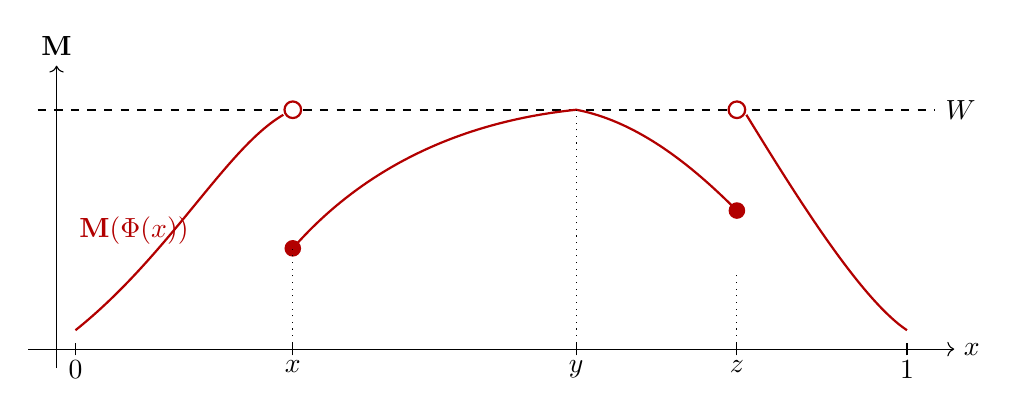
\begin{tikzpicture}[xscale=1.2, yscale=0.8]
      % Axes
      \draw[->] (-0.3, 0) -- (9.5, 0) node[right] {$x$};
      \draw[->] (0, -0.3) -- (0, 4.5) node[above] {$\mathbf{M}$};
      % Tick marks
      \draw (0.2, -0.1) -- (0.2, 0.1) node[below=3pt] {$0$};
      \draw (9.0, -0.1) -- (9.0, 0.1) node[below=3pt] {$1$};
      % Width line W
      \draw[dashed, thick] (-0.2, 3.8) -- (9.3, 3.8) node[right] {$W$};
      % Mass curve with discontinuities at x and z
      % Segment 1: 0 to x (open circle at W)
      \draw[thick, bindA] (0.2, 0.3) .. controls (1.2, 1.5) and (1.8, 3.2) .. (2.4, 3.72);
      \node[circle, fill=white, draw=bindA, thick, inner sep=0, minimum size=6pt] at (2.5, 3.8) {};
      % Segment 2: x to z, passing through y at W
      \node[circle, fill=bindA, inner sep=0, minimum size=6pt] at (2.5, 1.6) {};
      \draw[thick, bindA] (2.5, 1.6) .. controls (3.2, 2.8) and (4.2, 3.6) .. (5.5, 3.8)
        .. controls (6.2, 3.6) and (6.8, 2.8) .. (7.2, 2.2);
      \node[circle, fill=bindA, inner sep=0, minimum size=6pt] at (7.2, 2.2) {};
      % Segment 3: z to 1 (open circle at W)
      \node[circle, fill=white, draw=bindA, thick, inner sep=0, minimum size=6pt] at (7.2, 3.8) {};
      \draw[thick, bindA] (7.3, 3.72) .. controls (7.8, 2.5) and (8.5, 0.8) .. (9.0, 0.3);
      \node[bindA, above left] at (1.5, 1.5) {$\mathbf{M}(\Phi(x))$};
      % Mark x
      \draw (2.5, -0.1) -- (2.5, 0.1) node[below=3pt] {$x$};
      \draw[dotted, thin] (2.5, 0.1) -- (2.5, 1.6);
      % Mark y (at W)
      \draw (5.5, -0.1) -- (5.5, 0.1) node[below=3pt] {$y$};
      \draw[dotted, thin] (5.5, 0.1) -- (5.5, 3.8);
      % Mark z
      \draw (7.2, -0.1) -- (7.2, 0.1) node[below=3pt] {$z$};
      \draw[dotted, thin] (7.2, 0.1) -- (7.2, 1.2);
    \end{tikzpicture}
    \caption{The mass function $x \mapsto \mathbf{M}(\Phi(x))$ of a sweepout with jump discontinuities. All three marked points are critical ($M(x) = M(y) = M(z) = W$). The point $x$ is left critical only ($x \in \mathfrak{m}_L \setminus \mathfrak{m}_R$): the mass approaches $W$ from the left but drops after the jump. The point $z$ is right critical only ($z \in \mathfrak{m}_R \setminus \mathfrak{m}_L$): the mass approaches $W$ from the right but not from the left. The point $y$ is both left and right critical ($y \in \mathfrak{m}_L \cap \mathfrak{m}_R$), illustrating that the intersection need not be empty.}
    \label{fig:critical-points}
\end{figure}

\begin{definition}[Critical set~{\cite[Definition~1.5]{CLS22}}]\label{def:critical-set}
Given a sweepout $\Phi$, define
\[
M(x) = \limsup_{r \to 0} \{\mathbf{M}(\Phi(y)): |y-x| < r\}.
\]
If $\Phi$ is an optimal sweepout, the \emph{critical domain of $\Phi$} is
\[
\mathfrak{m}(\Phi)=\{ x \in [0,1]: M(x) =W \}.
\]
A point $x \in \mathfrak{m}(\Phi)$ is a \emph{left critical point} if there exists a sequence $x_i \nearrow x$ with $\mathbf{M}(\Phi(x_i)) \to W$, and a \emph{right critical point} if there exists $x_i \searrow x$ with $\mathbf{M}(\Phi(x_i)) \to W$. We denote by $\mathfrak{m}_L(\Phi)$ and $\mathfrak{m}_R(\Phi)$ the sets of left and right critical points, respectively. Note that $\mathfrak{m}(\Phi) = \mathfrak{m}_L(\Phi) \cup \mathfrak{m}_R(\Phi)$, and the intersection $\mathfrak{m}_L(\Phi) \cap \mathfrak{m}_R(\Phi)$ need not be empty.

A sequence $x_i \to x_0 \in \mathfrak{m}(\Phi)$ is a \emph{min-max sequence} if $|\partial^*\Omega(x_i)|$ converges in the varifold sense to a varifold $V$ with $\|V\|(M) = W$.
\end{definition}

\begin{definition}[Excessive intervals and points~{\cite[Definition~2.1]{CLS22}}]\label{def:excessive-interval}
Suppose $\{\Phi(x) = \partial\Omega(x)\}$ is a sweepout. Given a connected interval $I \subset [0,1]$
(which may be open, closed, or half-open), we say that $\{\Phi^I(x) = \partial\Omega^I(x)\}_{x\in \bar{I}}$
is an \emph{$I$-replacement family for $\Phi$} if
$x \mapsto \Omega^I(x)$ is flat continuous on $\bar{I}$,
$\Omega^I(a) = \Omega(a)$, $\Omega^I(b) = \Omega(b)$ at the endpoints, and for all $x \in I$,
\[
\limsup_{I \ni y \to x} \mathbf{M}(\Phi^I(y)) < W,
\]
where $W := \sup_x \mathbf{M}(\Phi(x))$.

We say that a connected interval $I$ is an \emph{excessive interval for $\Phi$} if there exists an $I$-replacement family
for $\Phi$. A point $x$ is called \emph{left excessive for $\Phi$} (resp.\ \emph{right excessive}) if there exists an excessive interval $I$ with
$(x-\varepsilon, x] \subset I$ (resp.\ $[x, x+\varepsilon) \subset I$) for some $\varepsilon > 0$.
\end{definition}

\begin{figure}[H]
    \centering
    % ==================== Top: original mass curve ====================
    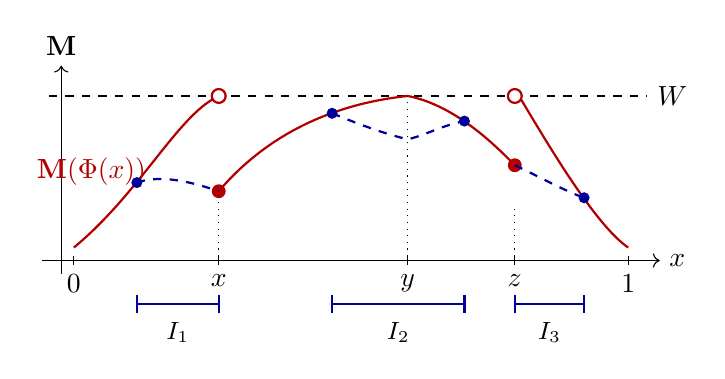
\begin{tikzpicture}[xscale=0.8, yscale=0.55]
      % Axes
      \draw[->] (-0.3, 0) -- (9.5, 0) node[right] {$x$};
      \draw[->] (0, -0.3) -- (0, 4.5) node[above] {$\mathbf{M}$};
      % Tick marks
      \draw (0.2, -0.1) -- (0.2, 0.1) node[below=3pt] {$0$};
      \draw (9.0, -0.1) -- (9.0, 0.1) node[below=3pt] {$1$};
      % Width line W
      \draw[dashed, thick] (-0.2, 3.8) -- (9.3, 3.8) node[right] {$W$};
      % Segment 1: 0 to x (open circle at W)
      \draw[thick, bindA] (0.2, 0.3) .. controls (1.2, 1.5) and (1.8, 3.2) .. (2.4, 3.72);
      \node[circle, fill=white, draw=bindA, thick, inner sep=0, minimum size=5pt] at (2.5, 3.8) {};
      % Segment 2: x to z, passing through y at W
      \node[circle, fill=bindA, inner sep=0, minimum size=5pt] at (2.5, 1.6) {};
      \draw[thick, bindA] (2.5, 1.6) .. controls (3.2, 2.8) and (4.2, 3.6) .. (5.5, 3.8)
        .. controls (6.2, 3.6) and (6.8, 2.8) .. (7.2, 2.2);
      \node[circle, fill=bindA, inner sep=0, minimum size=5pt] at (7.2, 2.2) {};
      % Segment 3: z to 1 (open circle at W)
      \node[circle, fill=white, draw=bindA, thick, inner sep=0, minimum size=5pt] at (7.2, 3.8) {};
      \draw[thick, bindA] (7.3, 3.72) .. controls (7.8, 2.5) and (8.5, 0.8) .. (9.0, 0.3);
      \node[bindA, above left] at (1.5, 1.5) {$\mathbf{M}(\Phi(x))$};
      % Mark x
      \draw (2.5, -0.1) -- (2.5, 0.1) node[below=3pt] {$x$};
      \draw[dotted, thin] (2.5, 0.1) -- (2.5, 1.6);
      % Mark y (at W)
      \draw (5.5, -0.1) -- (5.5, 0.1) node[below=3pt] {$y$};
      \draw[dotted, thin] (5.5, 0.1) -- (5.5, 3.8);
      % Mark z
      \draw (7.2, -0.1) -- (7.2, 0.1) node[below=3pt] {$z$};
      \draw[dotted, thin] (7.2, 0.1) -- (7.2, 1.2);
      % === I_x replacement (left of x) ===
      \draw[thick, blue!60!black] (1.2, -1.0) -- (2.5, -1.0);
      \draw[thick, blue!60!black] (1.2, -1.2) -- (1.2, -0.8);
      \draw[thick, blue!60!black] (2.5, -1.2) -- (2.5, -0.8);
      \node[below, font=\small] at (1.85, -1.2) {$I_1$};
      \node[circle, fill=blue!60!black, inner sep=0, minimum size=4pt] at (1.2, 1.80) {};
      \draw[thick, blue!60!black, dashed] (1.2, 1.80) .. controls (1.6, 2.0) and (2.1, 1.8) .. (2.5, 1.6);
      % === I_y replacement (both sides of y) ===
      \draw[thick, blue!60!black] (4.3, -1.0) -- (6.4, -1.0);
      \draw[thick, blue!60!black] (4.3, -1.2) -- (4.3, -0.8);
      \draw[thick, blue!60!black] (6.4, -1.2) -- (6.4, -0.8);
      \node[below, font=\small] at (5.35, -1.2) {$I_2$};
      \node[circle, fill=blue!60!black, inner sep=0, minimum size=4pt] at (4.3, 3.40) {};
      \node[circle, fill=blue!60!black, inner sep=0, minimum size=4pt] at (6.4, 3.22) {};
      \draw[thick, blue!60!black, dashed] (4.3, 3.40) .. controls (4.8, 3.1) and (5.2, 2.9) .. (5.5, 2.8)
        .. controls (5.8, 2.9) and (6.0, 3.1) .. (6.4, 3.22);
      % === I_z replacement (right of z) ===
      \draw[thick, blue!60!black] (7.2, -1.0) -- (8.3, -1.0);
      \draw[thick, blue!60!black] (7.2, -1.2) -- (7.2, -0.8);
      \draw[thick, blue!60!black] (8.3, -1.2) -- (8.3, -0.8);
      \node[below, font=\small] at (7.75, -1.2) {$I_3$};
      \node[circle, fill=blue!60!black, inner sep=0, minimum size=4pt] at (8.3, 1.45) {};
      \draw[thick, blue!60!black, dashed] (7.2, 2.2) .. controls (7.5, 2.0) and (8.0, 1.6) .. (8.3, 1.45);
    \end{tikzpicture}

    \smallskip
    (a)
    \vspace{0.5em}

    % ==================== (b) Monotone increasing ====================
    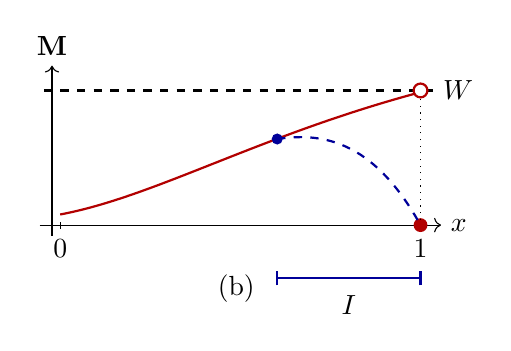
\begin{tikzpicture}[xscale=0.52, yscale=0.45]
      % Axes
      \draw[->] (-0.3, 0) -- (9.5, 0) node[right] {$x$};
      \draw[->] (0, -0.3) -- (0, 4.5) node[above] {$\mathbf{M}$};
      % Tick marks
      \draw (0.2, -0.1) -- (0.2, 0.1) node[below=3pt] {$0$};
      \draw (9.0, -0.1) -- (9.0, 0.1) node[below=3pt] {$1$};
      % Width line W
      \draw[dashed, thick] (-0.2, 3.8) -- (9.3, 3.8) node[right] {$W$};
      % Monotone increasing curve: 0 → W (open circle at top, filled at 0)
      \draw[thick, bindA] (0.2, 0.3) .. controls (2.5, 0.8) and (5.0, 2.5) .. (8.9, 3.72);
      \node[circle, fill=white, draw=bindA, thick, inner sep=0, minimum size=5pt] at (9.0, 3.8) {};
      \node[circle, fill=bindA, inner sep=0, minimum size=5pt] at (9.0, 0) {};
      \draw[dotted, thin] (9.0, 0.15) -- (9.0, 3.65);
      % Replacement interval I and curve
      \draw[thick, blue!60!black] (5.5, -1.5) -- (9.0, -1.5);
      \draw[thick, blue!60!black] (5.5, -1.7) -- (5.5, -1.3);
      \draw[thick, blue!60!black] (9.0, -1.7) -- (9.0, -1.3);
      \node[below] at (7.25, -1.7) {$I$};
      \node[circle, fill=blue!60!black, inner sep=0, minimum size=4pt] at (5.5, 2.43) {};
      \draw[thick, blue!60!black, dashed] (5.5, 2.43) .. controls (6.5, 2.6) and (7.8, 2.5) .. (9.0, 0);
      \node at (4.5, -1.8) {(b)};
    \end{tikzpicture}
    \hfill
    % ==================== (c) Monotone decreasing ====================
    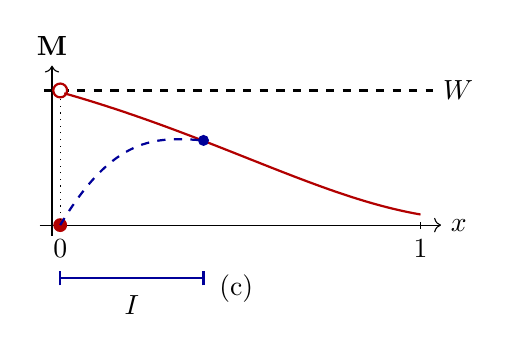
\begin{tikzpicture}[xscale=0.52, yscale=0.45]
      % Axes
      \draw[->] (-0.3, 0) -- (9.5, 0) node[right] {$x$};
      \draw[->] (0, -0.3) -- (0, 4.5) node[above] {$\mathbf{M}$};
      % Tick marks
      \draw (0.2, -0.1) -- (0.2, 0.1) node[below=3pt] {$0$};
      \draw (9.0, -0.1) -- (9.0, 0.1) node[below=3pt] {$1$};
      % Width line W
      \draw[dashed, thick] (-0.2, 3.8) -- (9.3, 3.8) node[right] {$W$};
      % Monotone decreasing curve: open circle at W, filled at 0, then decreasing
      \node[circle, fill=white, draw=bindA, thick, inner sep=0, minimum size=5pt] at (0.2, 3.8) {};
      \node[circle, fill=bindA, inner sep=0, minimum size=5pt] at (0.2, 0) {};
      \draw[dotted, thin] (0.2, 0.15) -- (0.2, 3.65);
      \draw[thick, bindA] (0.3, 3.72) .. controls (4.0, 2.5) and (6.5, 0.8) .. (9.0, 0.3);
      % Replacement interval I and curve
      \draw[thick, blue!60!black] (0.2, -1.5) -- (3.7, -1.5);
      \draw[thick, blue!60!black] (0.2, -1.7) -- (0.2, -1.3);
      \draw[thick, blue!60!black] (3.7, -1.7) -- (3.7, -1.3);
      \node[below] at (1.95, -1.7) {$I$};
      \draw[thick, blue!60!black, dashed] (0.2, 0) .. controls (1.5, 2.5) and (2.5, 2.5) .. (3.7, 2.39);
      \node[circle, fill=blue!60!black, inner sep=0, minimum size=4pt] at (3.7, 2.39) {};
      \node at (4.5, -1.8) {(c)};
    \end{tikzpicture}
    \caption{Excessive intervals and $I$-replacement families. (a)~A mass curve with critical points $x \in \mathfrak{m}_L \setminus \mathfrak{m}_R$, $y \in \mathfrak{m}_L \cap \mathfrak{m}_R$, $z \in \mathfrak{m}_R \setminus \mathfrak{m}_L$; blue dashed curves indicate replacement families on $I_1, I_2, I_3$ with mass strictly below $W$. (b)~A left-critical-only point at $x = 1$. (c)~A right-critical-only point at $x = 0$. See Remark~\ref{rem:excessive-critical}.}
    \label{fig:excessive-remark}
\end{figure}

\begin{remark}\label{rem:excessive-critical}
The left/right excessive distinction is non-trivial only on the side where the mass approaches $W$. Concretely, let $x \in \mathfrak{m}(\Phi)$ be an interior point of $[0,1]$.
\begin{itemize}
    \item If $x \in \mathfrak{m}_L \setminus \mathfrak{m}_R$ (left critical only), then left excessive is non-trivial while right excessive is automatic: the mass to the right of $x$ is already strictly below $W$, so any excessive interval $I \supset (x - \varepsilon, x]$ can be extended to $I' \supset (x - \varepsilon, x + \delta]$ by keeping the original $\Omega$ on the right.
    \item Symmetrically, if $x \in \mathfrak{m}_R \setminus \mathfrak{m}_L$, then right excessive is non-trivial while left excessive is automatic.
    \item Both directions are non-trivial only at points in $\mathfrak{m}_L \cap \mathfrak{m}_R$.
\end{itemize}
In particular, for interior critical points, the non-excessive condition imposes a genuine constraint only on the side from which the mass approaches $W$.

At the endpoints, only one side exists: $x = 0$ can only belong to $\mathfrak{m}_R$ and $x = 1$ can only belong to $\mathfrak{m}_L$. Since there is no opposite side to extend into, the excessive condition on that sole critical side is genuinely non-trivial (see Figure~\ref{fig:excessive-remark}(b)--(c)).
\end{remark}


A sweepout is called \emph{non-excessive} if no critical point is excessive on its critical side. The key advantage of non-excessiveness is that it enables \emph{local} contradiction arguments: if a property (such as integrality or regularity) fails at a point $p \in \spt\|V\|$, one can construct an $I$-replacement that lowers mass in a neighbourhood of $p$, producing an excessive interval and contradicting the non-excessive hypothesis. This is in contrast with classical min-max, where one must build a \emph{global} competitor sweepout of smaller width. We will exploit this local mechanism directly in the integrality (Section~\ref{sec:integrality}) and regularity (Section~\ref{sec:regularity}) arguments.

The fundamental result of~\cite{CLS22} is that non-excessive sweepouts exist:

\begin{theorem}[Existence of non-excessive sweepouts~{\cite[Theorem~2.2]{CLS22}}]\label{thm:non-excessive-existence}
Let $(M^{n+1},g)$ be a closed Riemannian manifold with $2\leq n\leq 6$. There exists an (ONVP) sweepout $\Psi$ such that every $x\in \mathfrak{m}_L(\Psi)$ is not left excessive and every $x \in \mathfrak{m}_R(\Psi)$ is not right excessive.
\end{theorem}

We denote by $\Snm$ the collection of all non-excessive sweepouts. Any optimal sweepout produces a stationary varifold via the standard pull-tight argument:

\begin{proposition}[Stationary varifolds from optimal sweepouts~{\cite[Proposition~1.4]{CL03}}]\label{thm:CLS-stationary}
Let $(M^{n+1},g)$ be a closed Riemannian manifold with $n \geq 2$, and let $\Phi$ be an optimal sweepout with $\sup_x \mathbf{M}(\Phi(x)) = W$. Then there exists a stationary $n$-varifold $V$ in $M$ with $\mathbf{M}(V) = W$.
\end{proposition}

This follows from the pull-tight argument of Colding--de~Lellis~\cite{CL03}: varifold compactness produces a limit $V$ of slices whose masses approach $W$, and if every such limit were non-stationary, the tightening flow would produce a sweepout of strictly smaller width, contradicting optimality. The equality $\mathbf{M}(V) = W$ holds because $M$ is compact: varifold convergence $|\partial^*\Omega(x_i)| \to V$ in the compact Grassmannian bundle $G_n(M)$ gives $\mathbf{M}(V) = \lim_i \mathbf{M}(|\partial^*\Omega(x_i)|) = W$. The non-excessive condition is not used here; it enters in the analysis of the limit varifold below.

Let $\Phi$ be a non-excessive ONVP sweepout, $x_i \to x_0 \in \mathfrak{m}(\Phi)$ a min-max sequence, and $V$ the varifold limit of $|\partial^*\Omega(x_i)|$ given by Proposition~\ref{thm:CLS-stationary}. A key distinction arises depending on whether the mass of the limit slice $\mathbf{M}(\Phi(x_0))$ equals the width $W$.

\begin{figure}[ht]
    \centering
    % ==================== (a) X-shaped ====================
    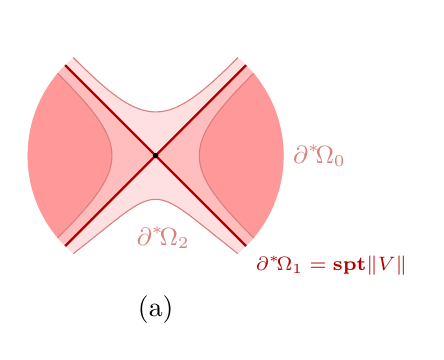
\begin{tikzpicture}[scale=0.65]
      % --- Ω_2 fill (outermost layer): left+right sectors ---
      \begin{scope}
      \clip (0,0) circle (2.5);
      \fill[red!40, opacity=0.3]
        ({2.5*cos(130)}, {2.5*sin(130)})
        .. controls (-0.2, 0.5) and (0.2, 0.5) ..
        ({2.5*cos(50)}, {2.5*sin(50)})
        -- (4, 4) -- (4, -4) --
        ({2.5*cos(310)}, {2.5*sin(310)})
        .. controls (-0.2, -0.5) and (0.2, -0.5) ..
        ({2.5*cos(230)}, {2.5*sin(230)})
        -- (-4, -4) -- (-4, 4) -- cycle;
      \end{scope}

      % --- Ω_0 outer fill (middle layer): right of right curve ---
      \begin{scope}
      \clip (0,0) circle (2.5);
      \fill[red!40, opacity=1.0]
        ({2.5*cos(40)}, {2.5*sin(40)})
        .. controls (0.5, 0.2) and (0.5, -0.2) ..
        ({2.5*cos(320)}, {2.5*sin(320)})
        -- (4, -4) -- (4, 4) -- cycle;
      \end{scope}

      % --- Ω_0 outer fill (middle layer): left of left curve ---
      \begin{scope}
      \clip (0,0) circle (2.5);
      \fill[red!40, opacity=1.0]
        ({2.5*cos(140)}, {2.5*sin(140)})
        .. controls (-0.5, 0.2) and (-0.5, -0.2) ..
        ({2.5*cos(220)}, {2.5*sin(220)})
        -- (-4, -4) -- (-4, 4) -- cycle;
      \end{scope}

      % --- Ω_1 fill (innermost layer): right wedge of X ---
      \begin{scope}
      \clip (0,0) circle (2.5);
      \fill[red!40, opacity=0.5]
        (0,0) -- ({4*cos(45)}, {4*sin(45)}) -- ({4*cos(315)}, {4*sin(315)}) -- cycle;
      \end{scope}

      % --- Ω_1 fill (innermost layer): left wedge of X ---
      \begin{scope}
      \clip (0,0) circle (2.5);
      \fill[red!40, opacity=0.5]
        (0,0) -- ({4*cos(135)}, {4*sin(135)}) -- ({4*cos(225)}, {4*sin(225)}) -- cycle;
      \end{scope}

      % ∂*Ω_1: X (branches)
      \draw[bindA, thick] ({2.5*cos(225)}, {2.5*sin(225)}) -- (0,0) -- ({2.5*cos(45)}, {2.5*sin(45)});
      \draw[bindA, thick] ({2.5*cos(315)}, {2.5*sin(315)}) -- (0,0) -- ({2.5*cos(135)}, {2.5*sin(135)});
      \node[bindA, font=\scriptsize, anchor=north west] at ({2.5*cos(315)}, {2.5*sin(315)}) {$\partial^*\!\Omega_1 = \spt\|V\|$};

      % ∂*Ω_0: left+right curves (innermost)
      \draw[bindA!50, thin]
        ({2.5*cos(40)}, {2.5*sin(40)})
        .. controls (0.5, 0.2) and (0.5, -0.2) ..
        ({2.5*cos(320)}, {2.5*sin(320)});
      \draw[bindA!50, thin]
        ({2.5*cos(140)}, {2.5*sin(140)})
        .. controls (-0.5, 0.2) and (-0.5, -0.2) ..
        ({2.5*cos(220)}, {2.5*sin(220)});
      \node[bindA!50, font=\small] at (3.2, 0) {$\partial^*\!\Omega_0$};

      % ∂*Ω_2: top+bottom curves (outermost)
      \draw[bindA!50, thin]
        ({2.5*cos(130)}, {2.5*sin(130)})
        .. controls (-0.2, 0.5) and (0.2, 0.5) ..
        ({2.5*cos(50)}, {2.5*sin(50)});
      \draw[bindA!50, thin]
        ({2.5*cos(230)}, {2.5*sin(230)})
        .. controls (0.2, -0.5) and (-0.2, -0.5) ..
        ({2.5*cos(310)}, {2.5*sin(310)});
      \node[bindA!50, font=\small] at (0.15, -1.6) {$\partial^*\!\Omega_2$};

      % Intersection point
      \fill (0,0) circle (1.5pt);

      \node at (0, -3.0) {(a)};
    \end{tikzpicture}
    \qquad
    % ==================== (b) Y-shaped: 3 branches at 120° ====================
    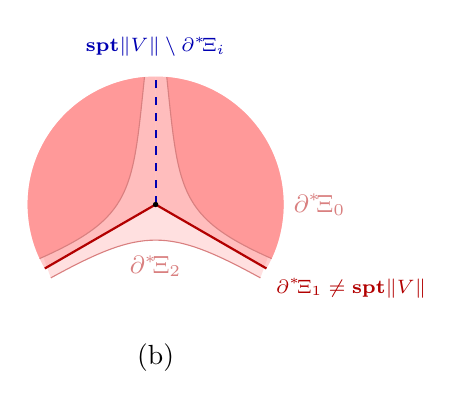
\begin{tikzpicture}[scale=0.65]
      % --- Ξ_2 fill (outermost layer): region above bottom arc ---
      \begin{scope}
      \clip (0,0) circle (2.5);
      \fill[red!40, opacity=0.3]
        ({2.5*cos(215)}, {2.5*sin(215)})
        .. controls (-0.25, -0.45) and (0.25, -0.45) ..
        ({2.5*cos(325)}, {2.5*sin(325)})
        -- (4, 4) -- (-4, 4) -- cycle;
      \end{scope}

      % --- Ξ_0 fill (middle layer): right of right arc ---
      \begin{scope}
      \clip (0,0) circle (2.5);
      \fill[red!40, opacity=1.0]
        ({2.5*cos(85)}, {2.5*sin(85)})
        .. controls (0.45, 0.25) and (0.45, -0.25) ..
        ({2.5*cos(335)}, {2.5*sin(335)})
        -- (4, -4) -- (4, 4) -- cycle;
      \end{scope}

      % --- Ξ_0 fill (middle layer): left of left arc ---
      \begin{scope}
      \clip (0,0) circle (2.5);
      \fill[red!40, opacity=1.0]
        ({2.5*cos(95)}, {2.5*sin(95)})
        .. controls (-0.45, 0.25) and (-0.45, -0.25) ..
        ({2.5*cos(205)}, {2.5*sin(205)})
        -- (-4, -4) -- (-4, 4) -- cycle;
      \end{scope}

      % --- Ξ_1 fill (innermost layer): right wedge ---
      \begin{scope}
      \clip (0,0) circle (2.5);
      \fill[red!40, opacity=0.5]
        (0,0) -- ({4*cos(330)}, {4*sin(330)}) -- ({4*cos(0)}, {4*sin(0)}) -- ({4*cos(90)}, {4*sin(90)}) -- cycle;
      \end{scope}

      % --- Ξ_1 fill (innermost layer): left wedge ---
      \begin{scope}
      \clip (0,0) circle (2.5);
      \fill[red!40, opacity=0.5]
        (0,0) -- ({4*cos(90)}, {4*sin(90)}) -- ({4*cos(150)}, {4*sin(150)}) -- ({4*cos(210)}, {4*sin(210)}) -- cycle;
      \end{scope}

      % ∂*Ξ_1: Y branches
      \draw[bindB, thick, dashed] (0,0) -- ({2.5*cos(90)}, {2.5*sin(90)});
      \node[bindB, font=\scriptsize, anchor=south] at (0, 2.7) {$\spt\|V\| \setminus \partial^*\!\Xi_i$};
      \draw[bindA, thick] (0,0) -- ({2.5*cos(210)}, {2.5*sin(210)});
      \draw[bindA, thick] (0,0) -- ({2.5*cos(330)}, {2.5*sin(330)});
      \node[bindA, font=\scriptsize, anchor=north west] at ({2.5*cos(330)}, {2.5*sin(330)}) {$\partial^*\!\Xi_1 \neq \spt\|V\|$};

      % ∂*Ξ_0: right wedge curve (between 330° and 90°, offset 5° inward)
      \draw[bindA!50, thin]
        ({2.5*cos(85)}, {2.5*sin(85)})
        .. controls (0.45, 0.25) and (0.45, -0.25) ..
        ({2.5*cos(335)}, {2.5*sin(335)});

      % ∂*Ξ_0: left wedge curve (between 90° and 210°, offset 5° inward)
      \draw[bindA!50, thin]
        ({2.5*cos(95)}, {2.5*sin(95)})
        .. controls (-0.45, 0.25) and (-0.45, -0.25) ..
        ({2.5*cos(205)}, {2.5*sin(205)});
      \node[bindA!50, font=\small] at (3.2, 0) {$\partial^*\!\Xi_0$};

      % ∂*Ξ_2: bottom wedge curve (between 210° and 330°, offset 5° inward)
      \draw[bindA!50, thin]
        ({2.5*cos(325)}, {2.5*sin(325)})
        .. controls (0.25, -0.45) and (-0.25, -0.45) ..
        ({2.5*cos(215)}, {2.5*sin(215)});
      \node[bindA!50, font=\small] at (0, -1.2) {$\partial^*\!\Xi_2$};

      % Intersection point
      \fill (0,0) circle (1.5pt);

      \node at (0, -3.0) {(b)};
    \end{tikzpicture}
    \caption{Cross-sections of non-trivial multiple junctions illustrating the mass cancellation dichotomy (Definition~\ref{def:mass-cancellation}); see also the $\alpha$-structure hypothesis in Section~\ref{sec:regularity}. \textbf{(a)}~No mass cancellation. \textbf{(b)}~Mass cancellation.}
    \label{fig:regularity-preview}
\end{figure}

Figure~\ref{fig:regularity-preview} illustrates this dichotomy near a non-trivial multiple junction of $\spt\|V\|$ (red branches). The lighter curves represent the approximating Caccioppoli boundaries $\partial^*\Omega(x_i)$, with shading indicating the nested Caccioppoli sets. When $\mathbf{M}(\Phi(x_0)) = W$ (panel~(a)), every branch of $\spt\|V\|$ is visible as a boundary component of $\partial^*\Omega(x_0)$. When $\mathbf{M}(\Phi(x_0)) < W$ (panel~(b)), the boundaries $\partial^*\Omega(x_i)$ from opposite sides approach and cancel in the sense of currents along the dashed blue branch, so that $\|V\|(B_r) > \mathrm{Per}(\Omega(x_0), B_r)$. This motivates the following definition.

\begin{definition}[Mass cancellation~{\cite[Section~6]{CLS22}}]\label{def:mass-cancellation}
Let $\Phi$ be a non-excessive (ONVP) sweepout with width $W$, and let $x_0 \in \mathfrak{m}(\Phi)$ be a critical point. We say that:
\begin{itemize}
    \item \emph{No mass cancellation} occurs at $x_0$ if $\mathbf{M}(\Phi(x_0)) = W$.
    \item \emph{Mass cancellation} occurs at $x_0$ if $\mathbf{M}(\Phi(x_0)) < W$.
\end{itemize}
\end{definition}

This dichotomy governs the integrality of the limit varifold; both cases are treated in Section~\ref{sec:integrality}.

Beyond stationarity and integrality, the non-excessive condition provides local geometric information about the limit varifold: critical slices are \emph{one-sided homotopic minimizers} in small balls, meaning they cannot be deformed to competitors of strictly smaller mass on either the inner or the outer side. This property is the mechanism through which non-excessiveness controls the regularity of the limit.

\begin{definition}[Homotopic minimizers~{\cite[Definition~1.4]{CLS22}}]\label{def:homotopic-minimizer}
Let $\Sigma = \partial^*\Omega$ be a Caccioppoli set in $M$, and let $U \subset M$ be an open set. We say
that $\Sigma$ is:
\begin{itemize}
    \item \emph{inner homotopic minimizing in $U$} if there is no Caccioppoli set $E \subset \Omega$
    with $E \triangle \Omega \subset U$ and $\mathrm{Per}(E, U) < \mathrm{Per}(\Omega, U)$ that can be connected to
    $\Omega$ by a continuous family of Caccioppoli sets in $U$;
    \item \emph{outer homotopic minimizing in $U$} if there is no Caccioppoli set $E \supset \Omega$
    with $E \triangle \Omega \subset U$ and $\mathrm{Per}(E, U) < \mathrm{Per}(\Omega, U)$ that can be connected to
    $\Omega$ by a continuous family of Caccioppoli sets in $U$;
    \item \emph{one-sided homotopic minimizing in $U$} if it is either inner or outer homotopic
    minimizing in $U$.
\end{itemize}
\end{definition}

\begin{definition}[Non-homotopic-minimizing points~{\cite[Definition~2.5]{CLS22}}]\label{def:hnm}
For a varifold $V$ arising from a min-max procedure, we define the set of \emph{non-homotopic-minimizing
points} by
\[
    \mathfrak{h}_{\mathrm{nm}}(V) := \left\{P \in \spt\|V\| : \begin{array}{l}
        \text{for all $r > 0$ small, $\spt\|V\| \cap B_r(P)$} \\
        \text{is not one-sided homotopic minimizing in $B_r(P)$}
    \end{array}\right\}.
\]
\end{definition}

The set $\mathfrak{h}_{\mathrm{nm}}(V)$ consists of points where the varifold fails to be one-sided minimizing in every neighborhood. A key consequence of~\cite[Proposition~3.1]{CLS22} is that for non-excessive sweepouts, this set is at most finite. In particular, the limit varifold is one-sided homotopic minimizing---hence stable---at all but finitely many points. This will be used in Section~\ref{sec:regularity} to verify the hypotheses of Wickramasekera's regularity theorem.

% !TEX root = ../../main.tex

\section{Regularity tools}\label{sec:regularity-tools}

The limit varifold $V$ from the min-max construction is stationary (Proposition~\ref{thm:CLS-stationary}). To promote it to a smooth embedded minimal hypersurface, we need a regularity theorem. The classical tool is the Schoen--Simon regularity theorem~\cite{SS81}, which applies to stable codimension~$1$ integral varifolds $V$ that are either \emph{almost minimizing} in sufficiently small annuli or satisfy $\mathcal{H}^{n-2}(\sing V) = 0$; under either condition, $\sing V = \varnothing$ for $2 \leq n \leq 6$. In the Almgren--Pitts theory~\cite{Alm65, Pit81} and its refinements by Colding--de~Lellis~\cite{CL03} and de~Lellis--Tasnady~\cite{DLT13}, the almost minimizing property is produced by a combinatorial selection procedure, and Schoen--Simon then gives full regularity.

In the non-excessive framework of Chodosh--Liokumovich--Spolaor~\cite{CLS22}, however, the geometric condition is \emph{one-sided homotopic minimization} (Definition~\ref{def:homotopic-minimizer}), which provides stability but does not immediately yield the almost minimizing condition in annuli that Schoen--Simon requires. In~\cite{CLS22}, this gap is bridged by invoking the Almgren--Pitts regularity theory as a black box. To close this gap without relying on Almgren--Pitts, we turn to Wickramasekera's regularity theorem~\cite{Wic14}, which applies to a broader class of stable codimension~$1$ integral varifolds defined by three hypotheses. We state them following~\cite[Section~2]{Wic14}, adapted from the Euclidean ball $B_2^{n+1}(0)$ to a Riemannian manifold.

\begin{definition}[The class $\mathcal{S}_\alpha$~{\cite[Section~2]{Wic14}}]\label{defn:class-S-alpha}
Fix $\alpha \in (0, 1)$. Let $V$ be an integral $n$-varifold on an open subset $U$ of a smooth $(n+1)$-dimensional Riemannian manifold $(N, g)$, with $\|V\|(U) < \infty$. We say $V \in \mathcal{S}_\alpha$ if $V$ satisfies the following three conditions:
\begin{itemize}
\item[$(\mathcal{S}1)$] \textbf{Stationarity.} $V$ has vanishing first variation:
\[
    \delta V(X) = \int \operatorname{div}_S X \, dV(x, S) = 0 \quad \text{for every } X \in \mathfrak{X}_c(U).
\]

\item[$(\mathcal{S}2)$] \textbf{Stability.} For each open set $\Omega \subset U$ such that $\sing V \cap \Omega = \varnothing$ (if $2 \leq n \leq 6$) or $\mathcal{H}^{n-7+\gamma}(\sing V \cap \Omega) = 0$ for every $\gamma > 0$ (if $n \geq 7$),
\[
    \int_{\reg V \cap \Omega} |A|^2 \zeta^2 \, d\mathcal{H}^n \leq \int_{\reg V \cap \Omega} |\nabla \zeta|^2 \, d\mathcal{H}^n \quad \text{for all } \zeta \in C^1_c(\reg V \cap \Omega),
\]
where $A$ is the second fundamental form of $\reg V$. Equivalently, $V$ has non-negative second variation for normal deformations compactly supported in $\Omega \setminus \sing V$.

\item[$(\mathcal{S}3)$] \textbf{$\alpha$-structural hypothesis.}\label{defn:alpha-structural} For each $Z \in \sing V$, there exists \emph{no} $\rho > 0$ such that $\spt\|V\| \cap B_\rho(Z)$ is equal to the union of finitely many embedded $C^{1,\alpha}$ hypersurfaces-with-boundary of $B_\rho(Z)$, all having a common $C^{1,\alpha}$ boundary containing $Z$, with no two intersecting except along their common boundary.
\end{itemize}
\end{definition}

\begin{figure}[ht]
    \centering
    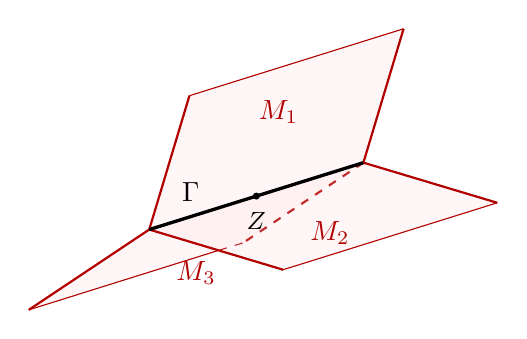
\begin{tikzpicture}[scale=0.85]
      % Edge Gamma: shared edge of three half-planes, with perspective
      \coordinate (A) at (-1.6,-0.5);
      \coordinate (B) at (1.6,0.5);

      % M_1 (upper half-plane): parallelogram above L
      \coordinate (A1) at ($(A)+(0.6,2.0)$);
      \coordinate (B1) at ($(B)+(0.6,2.0)$);

      % M_2 (lower-right half-plane): parallelogram to the right of L
      \coordinate (A2) at ($(A)+(2.0,-0.6)$);
      \coordinate (B2) at ($(B)+(2.0,-0.6)$);

      % M_3 (lower-left half-plane): parallelogram to the left of L
      \coordinate (A3) at ($(A)+(-1.8,-1.2)$);
      \coordinate (B3) at ($(B)+(-1.8,-1.2)$);

      % Intersection of A3--B3 with A--A2 (where M_3 passes behind M_2)
      \coordinate (I) at (-0.56,-0.81);

      % Fill and draw half-planes (back to front)
      % M_3 (behind): edges occluded by M_2 are dashed
      \fill[fillA, opacity=0.2] (A) -- (B) -- (B3) -- (A3) -- cycle;
      \draw[thick, bindA] (A) -- (A3);
      \draw[thick, bindA, dashed] (B) -- (B3);
      \draw[bindA] (A3) -- (I);
      \draw[bindA, dashed] (I) -- (B3);
      \node[bindA] at (-0.9,-1.15) {$M_3$};

      % M_1 (upper)
      \fill[fillA, opacity=0.2] (A) -- (B) -- (B1) -- (A1) -- cycle;
      \draw[thick, bindA] (A) -- (A1);
      \draw[thick, bindA] (B) -- (B1);
      \draw[bindA] (A1) -- (B1);
      \node[bindA] at (0.33,1.25) {$M_1$};

      % M_2 (lower-right)
      \fill[fillA, opacity=0.2] (A) -- (B) -- (B2) -- (A2) -- cycle;
      \draw[thick, bindA] (A) -- (A2);
      \draw[thick, bindA] (B) -- (B2);
      \draw[bindA] (A2) -- (B2);
      \node[bindA] at (1.1,-0.55) {$M_2$};

      % Edge Gamma (drawn on top)
      \draw[very thick] (A) -- (B);
      \node[above left] at ($(A)!0.28!(B)$) {$\Gamma$};

      % Singular point Z
      \coordinate (Z) at ($(A)!0.5!(B)$);
      \fill (Z) circle (1.5pt);
      \node[below] at ($(Z)+(0,-0.1)$) {\small $Z$};
    \end{tikzpicture}
    \caption{A configuration excluded by the $\alpha$-structural hypothesis $(\mathcal{S}3)$: three $C^{1,\alpha}$ hypersurfaces-with-boundary $M_1, M_2, M_3$ meeting along a common boundary $\Gamma$. The point $Z \in \Gamma$ is a singular point whose tangent cone is a union of three half-hyperplanes.}
    \label{fig:alpha-structural}
\end{figure}

\begin{remark}\label{rem:S-alpha-remarks}
\begin{enumerate}[label=\textup{(\roman*)}]
    \item Since $\reg V$ is open and dense in $\spt\|V\|$ by Allard's regularity theorem, $(\mathcal{S}2)$ is never vacuous; moreover $\mathcal{H}^{n-1}(\sing V) = 0$ trivially implies $(\mathcal{S}3)$, so $\mathcal{S}_\alpha$ contains all stable minimal hypersurfaces with small singular set~\cite[Remarks~(1)--(2) following~$(\mathcal{S}3)$]{Wic14}.
    \item For $V \in \mathcal{S}_\alpha$, hypothesis $(\mathcal{S}3)$ is equivalent to requiring that no tangent cone at a singular point is supported by \emph{three or more} distinct half-hyperplanes meeting along a common $(n-1)$-dimensional subspace; this equivalence relies on the Sheeting Theorem~\cite[Theorem~3.3]{Wic14} and the Minimum Distance Theorem~\cite[Theorem~3.4]{Wic14}; see also~\cite[Remark~(3) following~$(\mathcal{S}3)$]{Wic14}. The case of exactly two half-hyperplanes is already excluded by stationarity: a stationary cone supported on $N$ half-hyperplanes $P_1^+, \ldots, P_N^+$ meeting along a common edge $L$ satisfies the balancing condition $\sum_{j=1}^N \nu_j = 0$, where $\nu_j$ is the outward unit conormal of $P_j^+$ along $L$. When $N = 2$, this forces $\nu_1 = -\nu_2$, so the two half-hyperplanes form a single hyperplane and $Z$ is a regular point.
\end{enumerate}
\end{remark}

The main regularity result is:

\begin{theorem}[Regularity and Compactness~{\cite[Theorem~3.1, manifold version Theorem~6.1]{Wic14}}]\label{thm:wickramasekera}
    Let $(N^{n+1}, g)$ be a smooth Riemannian manifold and $\alpha \in (0, 1/2)$. If $V \in \mathcal{S}_\alpha$ on $N$ with $\|V\|(N) < \infty$, then:
    \begin{enumerate}[label=\textup{(\alph*)}]
        \item $\sing V = \varnothing$ if $2 \leq n \leq 6$;
        \item $\sing V$ is discrete if $n = 7$;
        \item $\mathcal{H}^{n-7+\gamma}(\sing V) = 0$ for each $\gamma > 0$ if $n \geq 8$.
    \end{enumerate}
    In particular, for $2 \leq n \leq 6$, $\spt\|V\|$ is a smooth embedded minimal hypersurface.
\end{theorem}

Wickramasekera's theorem strictly subsumes Schoen--Simon: if $\mathcal{H}^{n-2}(\sing V) = 0$, then $(\mathcal{S}3)$ holds vacuously (a junction of $C^{1,\alpha}$ hypersurfaces-with-boundary along an $(n-1)$-dimensional boundary would produce an $(n-1)$-dimensional singular set). Similarly, the almost minimizing property implies $\mathcal{H}^{n-2}(\sing V) = 0$ by Schoen--Simon, and thus implies $(\mathcal{S}3)$.


% !TEX root = ../../main.tex

\section{Density from one-sided minimality}\label{sec:one-sided-density}

In the mass cancellation case of the integrality argument (Section~\ref{subsec:integrality-cancel}), we need to show that the limit varifold $V$ has positive density everywhere on its support, even though the approximating Caccioppoli boundaries $|\partial^*\Omega_i|$ are not individually stationary. When the slices are one-sided area-minimizing, the density lower bound follows from the isoperimetric argument in Lin's theory of parametric obstacle problems~\cite{Lin85}, combined with a Portmanteau argument to pass the bound to the limit. Positive density then implies rectifiability of $V$ by Allard's theorem (Proposition~\ref{prop:allard-rectifiability}).

We remark that Lin's full regularity theory gives much stronger conclusions when one additionally assumes stationarity of each individual slice: if a Caccioppoli boundary $\partial^*\Omega$ is both stationary and one-sided area-minimizing, then $\spt\|\partial^*\Omega\|$ is a smooth embedded hypersurface outside a singular set of Hausdorff dimension at most $n - 7$ (discrete when $n = 7$), and the associated varifold is stable~\cite[Interior Regularity Theorem, \S0.2]{Lin85}; see also~\cite[Proposition~2.1]{Liu19}. In our setting, however, the individual slices $|\partial^*\Omega_i|$ are not stationary, so we cannot apply Lin's regularity theorem to them directly. Instead, we only use the one-sided minimality to obtain the mass ratio lower bound, which suffices for our purpose.


\begin{definition}[One-sided almost minimizers]\label{def:one-sided-perimeter-min}
Let $(M^{n+1}, g)$ be a Riemannian manifold, $\Omega$ a Caccioppoli set, $U \subset M$ open, and $\varepsilon \geq 0$.
We say $\Omega$ is \emph{locally one-sided inner $\varepsilon$-almost area-minimizing} in~$U$ if for every $q \in U$, every $\rho > 0$ with $B_\rho(q) \Subset U$, and every Caccioppoli set $F$ with $F \mathbin{\triangle} \Omega \Subset B_\rho(q)$ and $F \subset \Omega$,
\[
    \mathrm{Per}(\Omega, B_\rho(q)) \leq \mathrm{Per}(F, B_\rho(q)) + \varepsilon\,\rho^n.
\]
Similarly, $\Omega$ is \emph{locally one-sided outer $\varepsilon$-almost area-minimizing} in $U$ if the same holds for every $F \supset \Omega$ with $F \mathbin{\triangle} \Omega \Subset B_\rho(q)$.
When $\varepsilon = 0$ we recover the notion of \emph{locally one-sided area-minimizing}~\cite[Definition~1.10]{CLS22}.
\end{definition}

\begin{remark}[Compact containment is essential]\label{rem:compact-containment}
The condition $F \mathbin{\triangle} \Omega \Subset B_\rho(q)$ (compact containment) rather than $\subset B_\rho(q)$ is required to exclude the degenerate competitor $F = \Omega \setminus B_\rho(q)$. For this $F$, $\chi_F \equiv 0$ on the open ball, so $\mathrm{Per}(F, B_\rho(q)) = 0$; with $\subset$ the inequality would force $\mathrm{Per}(\Omega, B_\rho(q)) \leq \varepsilon\,\rho^n$ at all reduced boundary points, which is incompatible with density~$1$ at $\partial^*\Omega$. With $\Subset$, the competitor is required to agree with $\Omega$ in a neighborhood of $\partial B_\rho(q)$, which is the standard convention (e.g.,~\cite[Chapter~21]{Mag12}) and makes the half-space $\Omega = \{x_1 < 0\}$ one-sided $0$-almost area-minimizing in the usual sense.
\end{remark}

\begin{definition}[Two-sided perimeter decrease]\label{def:two-sided-decrease}
Let $(M^{n+1}, g)$ be a Riemannian manifold, $\Omega$ a Caccioppoli set, and $\varepsilon > 0$.
We say $\Omega$ admits a \emph{two-sided $\varepsilon$-perimeter decrease at $(q, \rho)$} if there exist Caccioppoli sets $F^-, F^+$ with
\[
    F^- \subset \Omega \subset F^+, \qquad F^\pm \mathbin{\triangle} \Omega \Subset B_\rho(q),
\]
such that
\[
    \mathrm{Per}(\Omega, B_\rho(q)) > \mathrm{Per}(F^\pm, B_\rho(q)) + \varepsilon\,\rho^n.
\]
Equivalently, $\Omega$ is \emph{not} locally one-sided $\varepsilon$-almost area-minimizing on either side at scale~$\rho$ near~$q$: neither the inner nor the outer almost-minimality inequality of Definition~\ref{def:one-sided-perimeter-min} holds at~$(q, \rho)$.
\end{definition}

This is precisely the Caccioppoli version of the parametric obstacle problem studied by Lin~\cite{Lin85}, whose thesis develops the regularity theory for hypersurfaces minimizing a parametric elliptic integrand subject to an obstacle constraint.
Lin's main formulation~\cite[\S0.2]{Lin85} assumes the obstacle domain has $C^{1,\alpha}$ boundary; this regularity is essential for his interior and boundary regularity theorems, but not for the mass ratio bounds that we use here.
Indeed, Lin~\cite[\S0.2, p.~12--13]{Lin85} also formulates a Caccioppoli version and proves an Equivalence Lemma showing that its solutions correspond to solutions of the integral-current formulation.


Federer's filling inequality~\cite[4.5.9(31)]{Fed69} guarantees that every $(n-1)$-cycle in $\mathbb{R}^{n+1}$ bounds an $n$-rectifiable set of controlled area, but we need the filling to be constrained to a subset (such as a geodesic ball). A Lipschitz retraction allows one to take a filling in the ambient space and project it back into the constraint set, with the Lipschitz constant controlling the area increase.

\begin{definition}[Lipschitz retract]\label{def:lipschitz-retract}
A closed set $A \subset \mathbb{R}^{n+1}$ (or a closed subset of a Riemannian manifold) is called a \emph{Lipschitz retract} if there exists a Lipschitz map $h\colon V \to A$ from an open neighborhood $V \supset A$ with $h|_A = \mathrm{id}_A$.
\end{definition}

For sufficiently small geodesic balls in a Riemannian manifold $(M,g)$, the closed ball $\overline{B}_\rho(q)$ is a Lipschitz retract: when $\rho$ is less than the convexity radius of $(M,g)$, the ball is geodesically convex, and the nearest-point projection
\[
    h(x) = \exp_q\!\Bigl(\min\bigl(1,\, \rho/d(x,q)\bigr)\, \exp_q^{-1}(x)\Bigr)
\]
defines a Lipschitz retraction $h\colon M \to \overline{B}_\rho(q)$ with Lipschitz constant depending only on $(M,g)$.

Combining the filling inequality~\cite[4.5.9(31)]{Fed69} with the constancy theorem~\cite[Theorem~26.27]{Sim83} in our codimension-one setting, we obtain the following competitor construction:

\begin{figure}[ht]
\centering
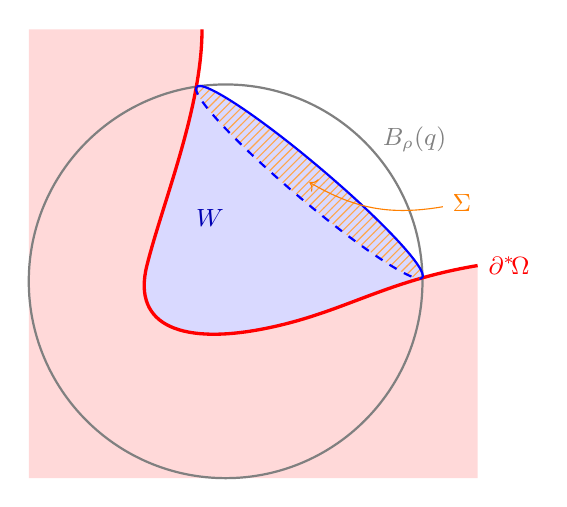
\begin{tikzpicture}
    % Step 0: Invisible paths to compute intersections and ellipse parameters
    \path[name path=circ0] (0,0) circle (2.5);
    \path[name path=bdry0] (-0.3,3.2) .. controls (-0.3,2.2) and (-0.8,1.0) .. (-1.0,0.2) .. controls (-1.2,-0.6) and (-0.5,-0.8) .. (0.5,-0.6) .. controls (1.5,-0.4) and (2.0,0.0) .. (3.2,0.2);
    \path[name intersections={of=circ0 and bdry0, by={A,B}}];
    \coordinate (M) at ($(A)!0.5!(B)$);
    \path let \p1 = ($(B)-(A)$) in
        \pgfextra{
            \pgfmathsetmacro{\smaj}{veclen(\x1,\y1)/2}
            \pgfmathsetmacro{\smin}{\smaj*0.12}
            \pgfmathsetmacro{\rang}{atan2(\y1,\x1)}
            \global\let\smaj\smaj
            \global\let\smin\smin
            \global\let\rang\rang
        };
    % Layer 1: Shading
    % Ω: shaded region to the left of ∂*Ω
    \fill[red!15] (-0.3,3.2) .. controls (-0.3,2.2) and (-0.8,1.0) .. (-1.0,0.2) .. controls (-1.2,-0.6) and (-0.5,-0.8) .. (0.5,-0.6) .. controls (1.5,-0.4) and (2.0,0.0) .. (3.2,0.2) -- (3.2,-2.5) -- (-2.5,-2.5) -- (-2.5,3.2) -- cycle;
    % W: region between ∂*Ω (right side) and chord A–B, inside ball
    \begin{scope}
        \clip (0,0) circle (2.5);
        % clip to non-Ω side of red curve
        \clip (-0.3,3.2) .. controls (-0.3,2.2) and (-0.8,1.0) .. (-1.0,0.2) .. controls (-1.2,-0.6) and (-0.5,-0.8) .. (0.5,-0.6) .. controls (1.5,-0.4) and (2.0,0.0) .. (3.2,0.2) -- (3.2,3.2) -- (-0.3,3.2) -- cycle;
        % fill the red-curve side of chord A–B
        \fill[blue!15] (A) -- (B) -- (-2.5,3.2) -- (-2.5,-2.5) -- (3.2,-2.5) -- cycle;
        % fill gap between chord A–B and the solid arc Σ
        \begin{scope}[shift=(M), rotate=\rang]
            \fill[blue!15] (\smaj pt,0) arc[start angle=0, end angle=-180, x radius=\smaj pt, y radius=\smin pt] -- cycle;
        \end{scope}
    \end{scope}
    % Layer 2: Lines (on top)
    \draw[gray, thick] (0,0) circle (2.5);
    \node[gray] at (2.4,1.8) {\small $B_\rho(q)$};
    % ∂*Ω
    \draw[red, very thick] (-0.3,3.2) .. controls (-0.3,2.2) and (-0.8,1.0) .. (-1.0,0.2) .. controls (-1.2,-0.6) and (-0.5,-0.8) .. (0.5,-0.6) .. controls (1.5,-0.4) and (2.0,0.0) .. (3.2,0.2);
    % Σ: solid front, dashed back, hatched interior (orange)
    \begin{scope}[shift=(M), rotate=\rang]
        \fill[pattern=north east lines, pattern color=orange!70] (0,0) ellipse[x radius=\smaj pt, y radius=\smin pt];
        \draw[blue, thick] (\smaj pt,0) arc[start angle=0, end angle=-180, x radius=\smaj pt, y radius=\smin pt];
        \draw[blue, thick, dashed] (\smaj pt,0) arc[start angle=0, end angle=180, x radius=\smaj pt, y radius=\smin pt];
    \end{scope}
    % Σ label outside with curved arrow to ellipse center
    \node[orange] (sigmalabel) at (3.0,1.0) {\small $\Sigma$};
    \draw[->, orange, thin] (sigmalabel) to[bend left=20] (M);
    % ∂*Ω label
    \node[red] at (3.6,0.2) {\small $\partial^*\!\Omega$};
    % W label in the blue shaded region
    \node[blue!70!black] at (-0.2,0.8) {\small $W$};
\end{tikzpicture}
\caption{Constructing the competitor $F = \Omega \cup W$ in $B_\rho(q)$: the filling surface $\Sigma$ spans the slice $\partial^*\Omega \cap \partial B_\rho(q)$, and $W$ is the Caccioppoli set bounded by $\partial^*\Omega \cap B_\rho(q)$ and $\Sigma$.}
\label{fig:caccioppoli-competitor}
\end{figure}

\begin{proposition}[Caccioppoli competitor in a geodesic ball~{\cite[4.5.9(31)]{Fed69}; \cite[Theorem~26.27]{Sim83}}]\label{prop:caccioppoli-competitor}
Let $(M^{n+1}, g)$ be a Riemannian manifold. There exist $r_0 > 0$ and $C = C(n, M, g) > 0$ such that for every Caccioppoli set $\Omega$, every $q \in M$, and a.e.\ $0 < \rho < r_0$, there exists a Caccioppoli set $F$ with $F \supset \Omega$, $F \mathbin{\triangle} \Omega \Subset B_\rho(q)$, and
\begin{equation}\label{eq:caccioppoli-competitor}
    \mathrm{Per}(F, B_\rho(q)) \leq C\,\mathcal{H}^{n-1}(\partial^*\Omega \cap \partial B_\rho(q))^{n/(n-1)}.
\end{equation}
The same holds with $F \subset \Omega$ in place of $F \supset \Omega$.
\end{proposition}

\begin{proof}
Fix $\rho$ in the full-measure set of radii where the coarea slice $\partial^*\Omega \cap \partial B_\rho(q)$ is $(n-1)$-rectifiable with no boundary as a current (by the coarea formula).
We first construct a competitor $F_{\rho'}$ with $F_{\rho'} \mathbin{\triangle} \Omega \subset \overline{B_{\rho'}(q)}$ for each $\rho' < \rho$ close to~$\rho$, then choose $\rho'$ so that $\overline{B_{\rho'}(q)} \Subset B_\rho(q)$ and the slice estimate transfers.

Federer's filling inequality~\cite[4.5.9(31)]{Fed69} states that every compactly supported $(n-1)$-cycle $Z$ in $\mathbb{R}^{n+1}$ bounds an $n$-dimensional integral current of mass at most $C\,\mathbf{M}(Z)^{n/(n-1)}$.
Applying this to the slice at scale $\rho'$ (viewed in normal coordinates) yields an $n$-dimensional surface $\Sigma_0$ spanning $\partial^*\Omega \cap \partial B_{\rho'}(q)$.
Since $\overline{B}_{\rho'}(q)$ is a Lipschitz retract (Definition~\ref{def:lipschitz-retract}), composing $\Sigma_0$ with the retraction $h_{\rho'} \colon M \to \overline{B}_{\rho'}(q)$ produces a surface $\Sigma_{\rho'} = (h_{\rho'})_\#\Sigma_0$ supported in $\overline{B}_{\rho'}(q)$ that still spans the slice, with
\[
    \mathcal{H}^n(\Sigma_{\rho'}) \leq \mathrm{Lip}(h_{\rho'})^n \, \mathcal{H}^n(\Sigma_0) \leq C\,\mathcal{H}^{n-1}(\partial^*\Omega \cap \partial B_{\rho'}(q))^{n/(n-1)}.
\]
Now $\Sigma_{\rho'}$ and $\partial^*\Omega \cap B_{\rho'}(q)$ share the same boundary, so their difference is an $n$-cycle supported in $\overline{B}_{\rho'}(q)$.
By the constancy theorem~\cite[Theorem~26.27]{Sim83}, this cycle equals $\partial\llrr{W_{\rho'}}$ for some Caccioppoli set $W_{\rho'} \subset \overline{B}_{\rho'}(q)$.
Setting $F_{\rho'} = \Omega \cup W_{\rho'}$ gives $F_{\rho'} \supset \Omega$ and $F_{\rho'} \mathbin{\triangle} \Omega = W_{\rho'} \subset \overline{B_{\rho'}(q)} \Subset B_\rho(q)$.
As in the original argument (Figure~\ref{fig:caccioppoli-competitor}), the boundary piece $\partial^*\Omega \cap B_{\rho'}(q)$ is absorbed into the interior of $F_{\rho'}$, so $\partial^* F_{\rho'} \cap B_\rho(q) \subset \Sigma_{\rho'} \cup (\partial^*\Omega \cap (B_\rho(q) \setminus \overline{B}_{\rho'}(q)))$ and
\begin{equation}\label{eq:Frho-prime-bound}
    \mathrm{Per}(F_{\rho'}, B_\rho(q)) \leq \mathcal{H}^n(\Sigma_{\rho'}) + \mathrm{Per}(\Omega, B_\rho(q) \setminus \overline{B}_{\rho'}(q)).
\end{equation}

Since the coarea function $\rho \mapsto \mathcal{H}^{n-1}(\partial^*\Omega \cap \partial B_\rho(q))$ is $L^1_{\mathrm{loc}}$ and $\mathrm{Per}(\Omega, B_\rho(q) \setminus \overline{B}_{\rho'}(q)) \to 0$ as $\rho' \nearrow \rho$ (by monotone convergence), for the Lebesgue-a.e.\ $\rho$ at which $\rho' \mapsto \mathcal{H}^{n-1}(\partial^*\Omega \cap \partial B_{\rho'}(q))$ is approximately continuous at $\rho$, we can choose $\rho' < \rho$ with
\begin{equation}\label{eq:Frho-prime-slice-bound}
    \mathcal{H}^{n-1}(\partial^*\Omega \cap \partial B_{\rho'}(q))^{n/(n-1)} + \mathrm{Per}(\Omega, B_\rho(q) \setminus \overline{B}_{\rho'}(q)) \leq 2\,\mathcal{H}^{n-1}(\partial^*\Omega \cap \partial B_{\rho}(q))^{n/(n-1)}.
\end{equation}
Setting $F := F_{\rho'}$ for any such $\rho'$, we obtain~\eqref{eq:caccioppoli-competitor} (with $C$ replaced by $2C$) and $F \mathbin{\triangle} \Omega \Subset B_\rho(q)$.
For the variant $F \subset \Omega$, take $F = \Omega \setminus W_{\rho'}$ instead; the same estimate holds.
\end{proof}

\begin{proposition}[Mass ratio lower bound from isoperimetric deficit]\label{prop:mass-ratio-lower-bound}
Let $(M^{n+1}, g)$ be a Riemannian manifold, $U \subset M$ open, $\Omega$ a Caccioppoli set, and $C_0, \varepsilon \geq 0$.
There exists $\varepsilon_0 = \varepsilon_0(n, M, g) > 0$ such that if $\varepsilon \leq \varepsilon_0$ and $\Omega$ satisfies the \emph{isoperimetric differential inequality}: for every $q \in \partial^*\Omega \cap U$ and a.e.\ $\rho > 0$ with $B_\rho(q) \Subset U$,
\begin{equation}\label{eq:isoperimetric-ode}
    \mathrm{Per}(\Omega, B_\rho(q)) \leq C_0\,\mathcal{H}^{n-1}(\partial^*\Omega \cap \partial B_\rho(q))^{n/(n-1)} + \varepsilon\,\rho^n,
\end{equation}
then for every $q \in \partial^*\Omega \cap U$ and every sufficiently small $\rho > 0$,
\begin{equation}\label{eq:mass-ratio-lower-bound}
    \mathrm{Per}(\Omega, B_\rho(q)) \geq c\,\rho^n,
\end{equation}
where $c > 0$ depends only on $n$, $C_0$, and $(M,g)$.
\end{proposition}

\begin{proof}
We adapt the isoperimetric argument of~\cite[\S0.3, p.~16]{Lin85}.
Let $q \in \partial^*\Omega \cap U$ and set $f(\rho) := \mathrm{Per}(\Omega, B_\rho(q))$.
By the coarea formula, $\mathcal{H}^{n-1}(\partial^*\Omega \cap \partial B_\rho(q)) = f'(\rho)$ for a.e.\ $\rho$, so~\eqref{eq:isoperimetric-ode} reads
\[
    f(\rho) \leq C_0\,f'(\rho)^{n/(n-1)} + \varepsilon\,\rho^n.
\]
Since $q \in \partial^*\Omega$, the density of $|\partial^*\Omega|$ at $q$ equals $1$, so $f(\rho)/(\omega_n\rho^n) \to 1$ as $\rho \to 0$.
In particular, for all sufficiently small $\rho$ we have $f(\rho) \geq (\omega_n/2)\,\rho^n$.
Choosing $\varepsilon_0 := \omega_n/4$, we have $\varepsilon\,\rho^n \leq f(\rho)/2$ for all such $\rho$, and therefore
\[
    f(\rho)/2 \leq C_0\,f'(\rho)^{n/(n-1)},
\]
i.e., $f(\rho)^{(n-1)/n} \leq C'\,f'(\rho)$.
Integrating this ODE gives $f(\rho) \geq c\,\rho^n$.
\end{proof}

\begin{corollary}\label{cor:mass-ratio-almost-min}
Let $C = C(n, M, g) > 0$ be the constant from Proposition~\ref{prop:caccioppoli-competitor}.
If $\Omega$ is locally one-sided (inner or outer) $\varepsilon$-almost area-minimizing in $U$ (Definition~\ref{def:one-sided-perimeter-min}) with $\varepsilon \leq \varepsilon_0$, then~\eqref{eq:isoperimetric-ode} holds with $C_0 = C$. In particular, the mass ratio lower bound~\eqref{eq:mass-ratio-lower-bound} holds.
\end{corollary}

\begin{proof}
By Proposition~\ref{prop:caccioppoli-competitor}, for a.e.\ $\rho$ there exists $F$ with $F \supset \Omega$ (resp.\ $F \subset \Omega$), $F \mathbin{\triangle} \Omega \subset B_\rho(q)$, and $\mathrm{Per}(F, B_\rho(q)) \leq C\,\mathcal{H}^{n-1}(\partial^*\Omega \cap \partial B_\rho(q))^{n/(n-1)}$.
By $\varepsilon$-almost minimality, $\mathrm{Per}(\Omega, B_\rho(q)) \leq \mathrm{Per}(F, B_\rho(q)) + \varepsilon\,\rho^n$, giving~\eqref{eq:isoperimetric-ode}.
\end{proof}

Combining the mass ratio bound with a Portmanteau argument, we obtain positive density for the limit varifold:

\begin{lemma}[Density from one-sided almost minimality]\label{lem:one-sided-density}
Let $(M^{n+1}, g)$ be a closed Riemannian manifold with $n \geq 2$, and let $\varepsilon_0 = \varepsilon_0(n, M, g) > 0$ be the constant from Proposition~\ref{prop:mass-ratio-lower-bound} (equivalently, Corollary~\ref{cor:mass-ratio-almost-min}).
Let $\Omega_i$ be Caccioppoli sets with $|\partial^*\Omega_i| \to V$ as varifolds.
Suppose that for some fixed $R > 0$, $p \in \spt\|V\|$, and $\varepsilon \leq \varepsilon_0$, each $\Omega_i$ is locally one-sided (inner or outer) $\varepsilon$-almost area-minimizing in $B_R(p)$ (Definition~\ref{def:one-sided-perimeter-min}; the side may vary with~$i$).
Then $\Theta(\|V\|, p) > 0$.
\end{lemma}

\begin{proof}
Assume $\Omega_i$ is locally one-sided outer $\varepsilon$-almost area-minimizing in $B_R(p)$ (the inner case is symmetric).
By Corollary~\ref{cor:mass-ratio-almost-min}, for every $q \in \partial^*\Omega_i \cap B_{R/2}(p)$ and $0 < r \leq R/4$,
\begin{equation}\label{eq:one-sided-mass-ratio}
    \|\partial^*\Omega_i\|(B_r(q)) \geq c\,r^n,
\end{equation}
where $c = c(n, M, g) > 0$.
Since $p \in \spt\|V\|$ and $|\partial^*\Omega_i| \to V$, for each small $r > 0$ there exist $q_i \in \partial^*\Omega_i \cap B_{r/2}(p)$ for all large~$i$.
Then $B_r(q_i) \subset B_{2r}(p)$ and~\eqref{eq:one-sided-mass-ratio} give
$\|\partial^*\Omega_i\|(B_{2r}(p)) \geq \|\partial^*\Omega_i\|(B_r(q_i)) \geq c\,r^n$.
Since $\overline{B}_{2r}(p)$ is closed, the Portmanteau theorem yields
$\|V\|(\overline{B}_{2r}(p)) \geq \limsup_{i \to \infty} \|\partial^*\Omega_i\|(\overline{B}_{2r}(p)) \geq c\,r^n$.
Dividing by $\omega_n (2r)^n$ and letting $r \to 0$ gives $\Theta(\|V\|, p) \geq c/(2^n \omega_n) > 0$.
\end{proof}

\subsection{The cancelled-mass case (open)}\label{subsec:cancelled-mass-open}

Lemma~\ref{lem:one-sided-density} establishes a density lower bound under the hypothesis of (all-scale) one-sided almost-minimality. In the mass-cancellation case of integrality (Section~\ref{subsec:integrality-cancel}), the cancelled mass $\mu_{\mathrm{c}} = \|V\| - |D\chi_{\Omega(x_0)}|$ is supported away from $\partial^*\Omega(x_0)$, and the corresponding density lower bound on $\spt\mu_{\mathrm{c}}$ is the main open input to integrality. We record the precise statement.

\begin{proposition}[Positive density on the cancelled mass]\label{prop:positive-density}
Let $(M^{n+1}, g)$ be a closed Riemannian manifold with $n \geq 2$, $\Phi$ a non-excessive ONVP sweepout with width $W$, $x_i \to x_0 \in \mathfrak{m}(\Phi)$ a min-max sequence, and $V$ the varifold limit of $|\partial^*\Omega(x_i)|$. Then
\[
    \Theta(\|V\|, p) > 0 \quad \text{for } \|V\|\text{-a.e.\ } p \in \spt\|V\|.
\]
\end{proposition}

By Allard's rectifiability theorem (Proposition~\ref{prop:allard-rectifiability}), Proposition~\ref{prop:positive-density} promotes $V$ to a rectifiable varifold; the sheet decomposition (Lemma~\ref{lem:sheet-decomposition}) then upgrades rectifiability to integer multiplicity, closing the integrality of $V$ in the mass-cancellation case (see Remark~\ref{rem:cancelled-mass-gap}).

We reduce Proposition~\ref{prop:positive-density} to the following claim.

\begin{claim}[Sweepout-wide replacement, open]\label{claim:sweepout-replacement}
Let $\Phi = \{\Omega_t\}_{t\in[0,1]}$ be a non-excessive ONVP sweepout with width $W$. Fix a min-max sequence $t_i \nearrow t_0 \in \mathfrak{m}(\Phi)$ with $|\partial^*\Omega_{t_i}| \to V$, and let $p \in \spt\|V\|$ with $p \in \mathrm{int}(\Omega_{t_0})$. There exist $\varepsilon = \varepsilon(n, M, g) > 0$ and, whenever $\|V\|(B_r(p)) < \varepsilon r^n$ for some $r > 0$ small, an $\mathcal{F}$-continuous, ONVP-nested family $\{\Omega^*_t\}_{t\in[0,1]}$ such that:
\begin{enumerate}[label=\textup{(\arabic*)}, leftmargin=2em]
    \item \textup{(Locality.)} $\Omega^*_t \mathbin{\triangle} \Omega_t \Subset B_r(p)$ for every $t \in [0,1]$.
    \item \textup{(Mass non-increase.)} $\mathrm{Per}(\Omega^*_t) \le \mathrm{Per}(\Omega_t)$ for every $t \in [0,1]$.
    \item \textup{(Strict decrease in the limit.)} If $|\partial^*\Omega^*_{t_i}| \to V^*$ as varifolds, then $\|V^*\|(B_r(p)) < \|V\|(B_r(p))$.
\end{enumerate}
\end{claim}

\begin{proof}[Proof of Proposition~\ref{prop:positive-density} assuming Claim~\ref{claim:sweepout-replacement}]
By contradiction, suppose $p \in \spt\|V\|$ has $\Theta(\|V\|, p) = 0$. By the monotonicity formula for stationary varifolds (Proposition~\ref{prop:p2-monotonicity}), it suffices to derive a contradiction from $\Theta(\|V\|, p) < \varepsilon$ for the constant $\varepsilon$ supplied by Claim~\ref{claim:sweepout-replacement}. After passing to a subsequence, fix $t_i \nearrow t_0 \in \mathfrak{m}(\Phi)$ with $|\partial^*\Omega_{t_i}| \to V$; by nestedness (Definition~\ref{def:p2-onvp}), $\Omega_{t_1} \subset \Omega_{t_2} \subset \cdots \subset \Omega_{t_0}$.

\textit{Case 1.} If $p \notin \overline{\Omega_{t_0}}$, then $B_\delta(p) \cap \overline{\Omega_{t_0}} = \varnothing$ for some $\delta > 0$, so by nestedness $|\partial^*\Omega_{t_i}|(B_\delta(p)) = 0$ for every $i$, giving $\|V\|(B_\delta(p)) = 0$ and contradicting $p \in \spt\|V\|$.

\textit{Case 2.} $p \in \overline{\Omega_{t_0}}$. By Lemma~\ref{lem:density-lower-bound} the density at points of $\partial^*\Omega_{t_0}$ is $\ge 1$, so we may assume $p \in \mathrm{int}(\Omega_{t_0})$. Choose $r > 0$ small enough that $\|V\|(B_r(p)) < \varepsilon r^n$; this is possible because $\Theta(\|V\|, p) < \varepsilon$. The hypotheses of Claim~\ref{claim:sweepout-replacement} are satisfied.

Apply Claim~\ref{claim:sweepout-replacement} to obtain $\{\Omega^*_t\}_{t\in[0,1]}$. By (1), $\Omega^*_t = \Omega_t$ outside $B_r(p)$, so $|\partial^*\Omega^*_{t_i}|$ and $|\partial^*\Omega_{t_i}|$ agree on $M \setminus B_r(p)$ for every $i$, and consequently $\|V^*\|(M \setminus B_r(p)) = \|V\|(M \setminus B_r(p))$. Setting $\delta := \|V\|(B_r(p)) - \|V^*\|(B_r(p)) > 0$ from (3), we obtain $\|V^*\|(M) = W - \delta$.

Choose an open interval $J \ni t_0$ in which $t_0$ is the only critical parameter of $\Phi$. For non-critical $t \in J$, (2) gives $\mathrm{Per}(\Omega^*_t) \le \mathrm{Per}(\Omega_t) < W$; for $t = t_0$,
\[
    \limsup_{s \to t_0} \mathbf{M}(\Phi^*(s)) \le \|V^*\|(M) = W - \delta < W.
\]
Therefore $\sup_{t \in J} \limsup_{s \to t} \mathbf{M}(\Phi^*(s)) < W$, which makes $J$ an excessive interval and $t_0$ excessive in the sense of Definition~\ref{def:excessive-interval}, contradicting the non-excessive property of $\Phi$.
\end{proof}

% !TEX root = ../../main.tex

\section{Integrality}\label{sec:integrality}

Integrality of the limit varifold is an essential input to the regularity argument: it ensures that tangent cones at singular points are integral cones, which constrains them to the junction configurations (wedges, folds, and higher-order junctions) needed to derive a contradiction when the $\alpha$-structural hypothesis (Definition~\ref{defn:alpha-structural}) fails (see Section~\ref{subsec:alpha-structural}). We begin by recalling the following criterion from de~Lellis--Tasnady~\cite{DLT13}, used in the no-mass-cancellation case (Section~\ref{subsec:integrality-no-cancel}):

\begin{proposition}[Varifolds vs.\ Caccioppoli set limits~{\cite[Proposition~A.1]{DLT13}}]\label{prop:p2-DLT-integrality}
    Let $\{\Omega^k\}$ be a sequence of Caccioppoli sets and $U$ an open subset of $M$. Assume that
    \begin{enumerate}[label=\textup{(\roman*)}]
        \item $D\chi_{\Omega^k} \to D\chi_\Omega$ in the sense of measures in $U$;
        \item $\mathrm{Per}(\Omega^k, U) \to \mathrm{Per}(\Omega, U)$
    \end{enumerate}
    for some Caccioppoli set $\Omega$. Then the varifolds $|\partial^*\Omega^k|$ converge to $|\partial^*\Omega|$ in the sense of varifolds.
\end{proposition}

The main result of this section is:

\begin{theorem}[Integrality of the limit varifold]\label{thm:integrality}
Let $(M^{n+1}, g)$ be a closed Riemannian manifold with $n \geq 2$, and let $\Phi$ be a non-excessive ONVP sweepout with width $W$. Let $x_i \to x_0 \in \mathfrak{m}(\Phi)$ be a min-max sequence and $V$ the varifold limit of $|\partial^*\Omega(x_i)|$.
\begin{enumerate}[label=\textup{(\alph*)}]
    \item If no mass cancellation occurs at $x_0$ (i.e., $\mathbf{M}(\Phi(x_0)) = W$), then $V = |\partial^*\Omega(x_0)|$ is an integral $n$-varifold.
    \item If mass cancellation occurs at $x_0$, then $\|V\|(A) \geq \mathcal{H}^n(\partial^*\Omega(x_0) \cap A)$ for every Borel $A$; moreover the restriction of $V$ to any open neighborhood of $\partial^*\Omega(x_0)$ that is disjoint from $\spt(\|V\| - |D\chi_{\Omega(x_0)}|)$ is integral. Integrality of $V$ on the full support $\spt\|V\|$ is conditional on Proposition~\ref{prop:positive-density} (positive density of the varifold limit $\|V\|$-a.e.\ on the cancelled mass $\mu_{\mathrm{c}} = \|V\| - |D\chi_{\Omega(x_0)}|$); see Remark~\ref{rem:cancelled-mass-gap}.
\end{enumerate}
\end{theorem}

Part~(a) is the de~Lellis--Tasnady criterion (Theorem~\ref{thm:integrality-mult-one} below); part~(b) is Lemma~\ref{lem:density-lower-bound} combined with the sheet decomposition (Lemma~\ref{lem:sheet-decomposition}) applied to $\mathcal{H}^n$-a.e.\ reduced boundary point, and with the gap in the cancelled mass spelled out in Remark~\ref{rem:cancelled-mass-gap}. Under the multiplicity-one conjecture (no mass cancellation), part~(a) applies and integrality is unconditional.

\subsection{The no-mass-cancellation case}\label{subsec:integrality-no-cancel}

\begin{theorem}[Integrality without mass cancellation]\label{thm:integrality-mult-one}
Assume no mass cancellation occurs at $x_0$, i.e., $\mathbf{M}(\Phi(x_0)) = W$. Then $V = |\partial^*\Omega(x_0)|$; in particular, $V$ is an integral varifold.
\end{theorem}

\begin{proof}
Since $\Phi$ is continuous in the flat topology, we have $\Omega(x_i) \to \Omega(x_0)$ in $L^1(M)$, so $D\chi_{\Omega(x_i)} \to D\chi_{\Omega(x_0)}$ weakly as measures. Moreover, the no-mass-cancellation hypothesis gives
\[
\mathrm{Per}(\Omega(x_i)) = \mathbf{M}(\Phi(x_i)) \to W = \mathbf{M}(\Phi(x_0)) = \mathrm{Per}(\Omega(x_0)).
\]
Both conditions of Proposition~\ref{prop:p2-DLT-integrality} are satisfied, so $V = |\partial^*\Omega(x_0)|$ is the integral varifold induced by the Caccioppoli boundary $\partial^*\Omega(x_0)$.
\end{proof}

\begin{figure}[ht]
    \centering
    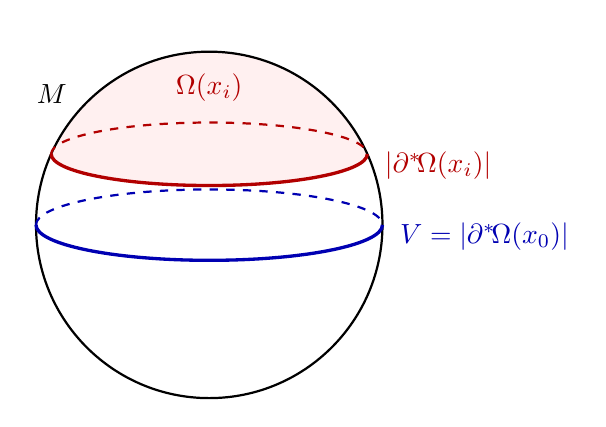
\begin{tikzpicture}[scale=1.0]
      \def\R{2.2}
      \def\h{0.9}
      \pgfmathsetmacro{\a}{sqrt(\R*\R - \h*\h)}
      \def\ew{0.4}
      \pgfmathsetmacro{\angR}{atan2(\h, \a)}

      % Fill cap (Omega): front ellipse arc + sphere arc over top
      \fill[fillA, opacity=0.4]
        (-\a, \h) arc (180:360:{\a} and {\ew})
        arc (\angR:180-\angR:\R);

      % Sphere outline
      \draw[thick] (0,0) circle (\R);

      % Boundary curve — front (solid)
      \draw[very thick, bindA] (-\a, \h) arc (180:360:{\a} and {\ew});
      % Boundary curve — back (dashed)
      \draw[thick, bindA, dashed] (-\a, \h) arc (180:0:{\a} and {\ew});

      % Equator (V) — front (solid)
      \draw[very thick, bindB] (-\R, 0) arc (180:360:{\R} and {0.45});
      % Equator (V) — back (dashed)
      \draw[thick, bindB, dashed] (-\R, 0) arc (180:0:{\R} and {0.45});

      % Labels
      \node[bindA] at (0, 1.75) {$\Omega(x_i)$};
      \node[bindA, right] at (\a+0.1, \h-0.15) {$|\partial^*\!\Omega(x_i)|$};
      \node[bindB, right] at (\R+0.1, -0.15) {$V = |\partial^*\!\Omega(x_0)|$};
      \node[above left] at ({-\R*cos(40)}, {\R*sin(40)}) {$M$};
    \end{tikzpicture}
    \caption{The no-mass-cancellation case on a closed manifold $M$. The shaded region is the Caccioppoli set $\Omega(x_i)$, with reduced boundary $|\partial^*\!\Omega(x_i)|$ (red). As $x_i \to x_0$, the varifolds $|\partial^*\!\Omega(x_i)|$ converge to $V = |\partial^*\!\Omega(x_0)|$ (blue), which is integral with multiplicity~$1$.}
    \label{fig:caccioppoli-set}
\end{figure}

The identification $V = |\partial^*\Omega(x_0)|$ has two important consequences beyond integrality: it tells us that $V$ is the boundary of a Caccioppoli set, which constrains the possible tangent cones and is used to verify the $\alpha$-structural hypothesis (Theorem~\ref{thm:alpha-hypo}); and it connects $V$ to the non-excessive structure of the sweepout, which provides the homotopic minimizing property and hence stability (Proposition~\ref{prop:stability}). Together with integrality, these are the inputs to Wickramasekera's regularity theorem (Section~\ref{sec:regularity}).

\subsection{The mass cancellation case}\label{subsec:integrality-cancel}

When mass cancellation occurs ($\mathbf{M}(\Phi(x_0)) < W$), we still have $\Omega(x_i) \to \Omega(x_0)$ in $L^1$, but the perimeter convergence condition in Proposition~\ref{prop:p2-DLT-integrality} fails:
\[
    \mathrm{Per}(\Omega(x_i)) \to W > \mathrm{Per}(\Omega(x_0)).
\]
The mass defect $W - \mathrm{Per}(\Omega(x_0)) > 0$ is carried by sheets of $\partial^*\Omega(x_i)$ that converge in pairs, cancelling in the flat topology but contributing positively to varifold mass. In particular, $V \neq |\partial^*\Omega(x_0)|$, and the integrality of $V$ does not follow from Proposition~\ref{prop:p2-DLT-integrality}.

The analysis splits $\|V\|$ into two parts via the comparison
\begin{equation}\label{eq:V-vs-D-chi-decomp}
    \|V\| = |D\chi_{\Omega(x_0)}| + \mu_{\mathrm{c}}, \qquad \mu_{\mathrm{c}} := \|V\| - |D\chi_{\Omega(x_0)}| \geq 0,
\end{equation}
where the non-negativity $\mu_{\mathrm{c}} \geq 0$ is established in Lemma~\ref{lem:density-lower-bound} by lower semicontinuity of total variation. The first part, $|D\chi_{\Omega(x_0)}|$, is the reduced-boundary component: at each $p \in \partial^*\Omega(x_0)$ density is $\geq 1$, and the sheet decomposition (Lemma~\ref{lem:sheet-decomposition}) further refines this to integer multiplicity. The second part, $\mu_{\mathrm{c}}$ (the \emph{cancelled mass}), satisfies $\mu_{\mathrm{c}}(M) = W - \mathrm{Per}(\Omega(x_0)) > 0$, is supported on the cancellation set where pairs of sheets of $\partial^*\Omega(x_i)$ converge to a common location; establishing its rectifiability and integer multiplicity is a separate problem discussed in Remark~\ref{rem:cancelled-mass-gap}.

The main tool for the $\partial^*\Omega(x_0)$-part is the following graphical decomposition lemma, which we state first.


\begin{lemma}[Lower bound on the limit mass by the flat limit]\label{lem:density-lower-bound}
Let $(M^{n+1}, g)$ be a closed Riemannian manifold with $n \geq 2$, and let $\Phi$ be a (not necessarily non-excessive) ONVP sweepout. Let $V$ be the varifold limit of $|\partial^*\Omega(x_i)|$ along a min-max sequence $x_i \to x_0 \in \mathfrak{m}(\Phi)$. Then
\begin{equation}\label{eq:V-dominates-DChi}
    \|V\|(A) \geq |D\chi_{\Omega(x_0)}|(A) = \mathcal{H}^n(\partial^*\Omega(x_0) \cap A)
    \quad \text{for every Borel } A \subset M.
\end{equation}
In particular, $\Theta(\|V\|, p) \geq 1$ for every $p \in \partial^*\Omega(x_0)$.
\end{lemma}

The inequality~\eqref{eq:V-dominates-DChi} follows from the lower semicontinuity of total variation under $L^1$ convergence, combined with the varifold convergence $|\partial^*\Omega(x_i)| \to V$; non-excessiveness is not used. The lemma gives positive density on $\partial^*\Omega(x_0) \cap \spt\|V\|$, on which the sheet decomposition (Lemma~\ref{lem:sheet-decomposition}) yields integer multiplicity. The complementary cancelled mass $\mu_{\mathrm{c}}$ from~\eqref{eq:V-vs-D-chi-decomp} is treated in Remark~\ref{rem:cancelled-mass-gap}.

% [Commented out: old proof by contradiction via isoperimetric replacement]
% \begin{proof}
% Since $V$ is stationary, the density $\Theta(\|V\|, p)$ exists at every point (Proposition~\ref{prop:p2-monotonicity}). We argue by contradiction: suppose there exists $p \in \spt\|V\|$ with $\Theta(\|V\|, p) = 0$. The strategy is as follows: the vanishing density forces $\Omega(x_i)$ to be nearly empty or nearly full inside small balls around~$p$. An isoperimetric replacement then produces a Caccioppoli set $E_i$ with strictly less perimeter, from which we construct an $I$-replacement family contradicting the non-excessiveness of $\Phi$.

% \medskip\noindent\textbf{Step~1} (Vanishing mass at small scales).
% Since the modified density ratio $e^{Cr}\,\omega_n^{-1} r^{-n}\|V\|(B_r(p))$ is non-decreasing in $r$ (Proposition~\ref{prop:p2-monotonicity}) and its limit as $r \to 0$ equals $\Theta(\|V\|, p) = 0$, we have
% \begin{gather}
%     \|V\|(B_r(p)) \leq \omega_n\, \alpha(r)\, r^n, \label{eq:density-vanishing} \\
%     \alpha(r) := e^{Cr}\,\omega_n^{-1} r^{-n}\|V\|(B_r(p)) \xrightarrow{r \to 0} 0. \notag
% \end{gather}
% In particular, $\|V\|(B_r(p)) = o(r^n)$. Now fix $\varepsilon > 0$ and choose $r_0 > 0$ so that $\alpha(r) < \varepsilon$ for all $r < r_0$. Since $r \mapsto \|V\|(B_r(p))$ is non-decreasing and hence has at most countably many jumps, $\|V\|(\partial B_r(p)) = 0$ for all but countably many $r$. For any such $r < r_0$, the Portmanteau theorem (as in~\eqref{eq:tilt-excess-transfer}) applied to the indicator $\mathbf{1}_{B_r(p)}$ gives
% \begin{equation}\label{eq:mass-transfer}
%     \mathrm{Per}(\Omega(x_i), B_r(p)) = \|\partial^*\Omega(x_i)\|(B_r(p)) \to \|V\|(B_r(p)) \quad \text{as } i \to \infty.
% \end{equation}
% Combining: for every $\varepsilon > 0$, there exists $r_0 > 0$ such that for each (good) $r < r_0$, there exists $i_0 = i_0(r, \varepsilon)$ with
% \begin{equation}\label{eq:per-small}
%     \mathrm{Per}(\Omega(x_i), B_r(p)) < \varepsilon\, \omega_n\, r^n \quad \text{for all } i \geq i_0.
% \end{equation}
%
% \medskip\noindent\textbf{Step~2} (Volume dichotomy via the isoperimetric inequality).
% Applying the relative isoperimetric inequality (Proposition~\ref{prop:relative-isoperimetric}) to $\Omega = \Omega(x_i)$ and using~\eqref{eq:per-small}:
% \begin{multline}\label{eq:volume-dichotomy}
%     \min\bigl(\mathcal{L}^{n+1}(\Omega(x_i) \cap B_r(p)),\;
%     \mathcal{L}^{n+1}(B_r(p) \setminus \Omega(x_i))\bigr) \\
%     \leq \bigl(C_I\,\varepsilon\,\omega_n\, r^n\bigr)^{(n+1)/n}
%     = C\,\varepsilon^{(n+1)/n}\, r^{n+1}
% \end{multline}
% for each good $r < \min(r_0, r_1)$ and all $i \geq i_0(r, \varepsilon)$. Since $\varepsilon > 0$ is arbitrary, the smaller side has volume $o(r^{n+1})$ as $r \to 0$ then $i \to \infty$: the set $\Omega(x_i) \cap B_r(p)$ is either nearly empty or nearly full.
%
% \medskip\noindent\textbf{Step~3} (Replacement and contradiction with non-excessiveness; cf.~\cite[Proposition~5.1]{DLT13}).
% By passing to a subsequence, we may assume $x_i \nearrow x_0$, so that $x_0 \in \mathfrak{m}_L(\Phi)$ and $x_0$ is not left excessive (Theorem~\ref{thm:non-excessive-existence}). By Step~2, passing to a further subsequence, either
% $\mathcal{L}^{n+1}(\Omega(x_i) \cap B_r(p)) = o(r^{n+1})$ (nearly empty) or
% $\mathcal{L}^{n+1}(B_r(p) \setminus \Omega(x_i)) = o(r^{n+1})$ (nearly full).
% Let $f_i(\rho)$ denote the smaller volume:
% \begin{equation}\label{eq:volume-small}
%     f_i(r) := \min\bigl(\mathcal{L}^{n+1}(\Omega(x_i) \cap B_r(p)),\;\mathcal{L}^{n+1}(B_r(p) \setminus \Omega(x_i))\bigr) = o(r^{n+1}).
% \end{equation}
%
% \emph{Finding a good radius.}
% The goal is to find a radius $\rho_i$ at which the boundary $\partial B_{\rho_i}(p)$ slices off less of $S_i$ than the isoperimetric inequality accounts for, so that we can construct a cheaper replacement.
%
% Let $S_i$ denote the side achieving the minimum in~\eqref{eq:volume-small}: $S_i = \Omega(x_i)$ if $\mathcal{L}^{n+1}(\Omega(x_i) \cap B_r(p)) \leq \mathcal{L}^{n+1}(B_r(p) \setminus \Omega(x_i))$, and $S_i = B_r(p) \setminus \Omega(x_i)$ otherwise, so that $f_i(\rho) = \mathcal{L}^{n+1}(S_i \cap B_\rho(p))$. The coarea formula gives
% \[
%     f_i'(\rho) = \mathcal{H}^n(\partial B_\rho(p) \cap S_i) \quad \text{for a.e.\ } \rho \in (0, r).
% \]
% Meanwhile, the relative isoperimetric inequality (Proposition~\ref{prop:relative-isoperimetric}) gives
% \begin{equation}\label{eq:isoperimetric-lower}
%     \mathrm{Per}(\Omega(x_i), B_\rho(p)) \geq c_n\, f_i(\rho)^{n/(n+1)},
% \end{equation}
% where $c_n = c_n(M, g, n) > 0$. We claim that there exists $\rho_i \in (r/2, r)$ with $f_i(\rho_i) > 0$ and
% \begin{equation}\label{eq:good-radius}
%     f_i'(\rho_i) < c_n\, f_i(\rho_i)^{n/(n+1)} \leq \mathrm{Per}(\Omega(x_i), B_{\rho_i}(p)).
% \end{equation}
% The first inequality in~\eqref{eq:good-radius} says that the ``slice cost'' $\mathcal{H}^n(\partial B_{\rho_i} \cap S_i)$ is strictly less than the perimeter inside $B_{\rho_i}$; at such a radius, replacing $\Omega(x_i)$ inside $B_{\rho_i}$ by filling in (or emptying out) $S_i$ reduces the total perimeter.
%
% To prove the claim, note that $p \in \spt\|V\|$ gives $\|V\|(B_{r/2}(p)) > 0$, so by~\eqref{eq:mass-transfer}, $\mathrm{Per}(\Omega(x_i), B_{r/2}(p)) > 0$ for $i$ large. This forces $f_i(\rho) > 0$ for all $\rho \geq r/2$: indeed, $\mathrm{Per} > 0$ gives a point $q \in \partial^*\Omega(x_i) \cap B_{r/2}(p)$, and at any reduced boundary point the set $\Omega(x_i)$ has $\mathcal{L}^{n+1}$-density $1/2$, so both $\Omega(x_i)$ and its complement have positive volume in $B_\rho(p) \supset B_{r/2}(p) \ni q$. Now suppose for contradiction that $f_i'(\rho) \geq c_n\, f_i(\rho)^{n/(n+1)}$ for a.e.\ $\rho \in (r/2, r)$. By the ODE comparison argument of~\cite[Proposition~5.1, Step~2]{DLT13}, setting $\varphi = f_i^{1/(n+1)}$ and dividing:
% \[
%     \varphi'(\rho) = \frac{f_i'(\rho)}{(n{+}1)\,f_i(\rho)^{n/(n+1)}} \geq \frac{c_n}{n{+}1} \quad \text{a.e.\ on } (r/2, r).
% \]
% Integrating over $(r/2, r)$:
% \[
%     f_i(r)^{1/(n+1)} \geq f_i(r/2)^{1/(n+1)} + \frac{c_n\, r}{2(n{+}1)} \geq \frac{c_n\, r}{2(n{+}1)},
% \]
% hence $f_i(r) \geq (c_n / (2(n{+}1)))^{n+1}\, r^{n+1}$. Since $(c_n/(2(n{+}1)))^{n+1} > 0$ is independent of $r$ and $i$, this contradicts $f_i(r) = o(r^{n+1})$ from~\eqref{eq:volume-small}, establishing the claim.
%
% \emph{Construction of the replacement.}
% Define the Caccioppoli set
% \[
%     E_i := \Omega(x_i) \triangle (S_i \cap \overline{B}_{\rho_i}(p)),
% \]
% which removes the small side $S_i$ from $\Omega(x_i)$ inside $B_{\rho_i}(p)$: when $S_i = \Omega(x_i)$, this gives $E_i = \Omega(x_i) \setminus \overline{B}_{\rho_i}$; when $S_i = B_r \setminus \Omega(x_i)$, it gives $E_i = \Omega(x_i) \cup \overline{B}_{\rho_i}$. In both cases, $E_i$ agrees with $\Omega(x_i)$ outside $B_{\rho_i}(p)$, while inside $B_{\rho_i}(p)$ the boundary $\partial^*\Omega(x_i) \cap B_{\rho_i}$ is replaced by the spherical slice $\partial B_{\rho_i} \cap S_i$ (see Figure~\ref{fig:isoperimetric-replacement}). For a.e.\ $\rho_i$ (chosen so that $\|V\|(\partial B_{\rho_i}(p)) = 0$ and $\mathcal{H}^{n-1}(\partial^*\Omega(x_i) \cap \partial B_{\rho_i}(p)) = 0$):
% \begin{align}
%     \mathrm{Per}(E_i, B_r(p))
%     &= \mathrm{Per}(\Omega(x_i),\, B_r(p) \setminus \overline{B}_{\rho_i})
%        + f_i'(\rho_i), \label{eq:per-replacement} \\
%     \mathrm{Per}(\Omega(x_i), B_r(p))
%     &= \mathrm{Per}(\Omega(x_i),\, B_r(p) \setminus \overline{B}_{\rho_i})
%        + \mathrm{Per}(\Omega(x_i), B_{\rho_i}(p)). \label{eq:per-original}
% \end{align}
% Therefore:
% \begin{alignat}{2}
%     &\mathrm{Per}(E_i) - \mathrm{Per}(\Omega(x_i)) \notag \\
%     ={}&\mathrm{Per}(E_i, B_r(p)) - \mathrm{Per}(\Omega(x_i), B_r(p))
%        &\qquad &\text{($E_i = \Omega(x_i)$ outside $B_r$)} \notag \\
%     ={}&f_i'(\rho_i) - \mathrm{Per}(\Omega(x_i), B_{\rho_i}(p))
%        &\qquad &\text{(by~\eqref{eq:per-replacement} and~\eqref{eq:per-original})} \notag \\
%     <{}&0.
%        &\qquad &\text{(by~\eqref{eq:good-radius})} \label{eq:per-decrease}
% \end{alignat}
%
% \begin{figure}[ht]
%     ... (figure omitted in comments)
% \end{figure}
%
% [Commented out: Cases 1, 2a, 2b setup — superseded by direct 2b(i)/2b(ii) dichotomy]
% \emph{Contradiction with non-excessiveness.}
% We have $\mathrm{Per}(E_i) < \mathrm{Per}(\Omega(x_i)) \leq W$ from~\eqref{eq:per-decrease}, and $\mathrm{Per}(\Omega(x_0)) < W$ by the mass cancellation hypothesis. The goal is to construct a flat-continuous $I$-replacement on $I = (x_i, x_0]$ with $\limsup_{I \ni y \to x}\mathbf{M}(\Phi^I(y)) < W$ for every $x \in I$, making $x_0$ left excessive and contradicting non-excessiveness (Definition~\ref{def:excessive-interval}). Note that $x_i \notin I$, so no limsup condition is imposed at~$x_i$; the difficulty is that $\mathrm{Per}(\Omega(x_i))$ may equal~$W$. We distinguish two cases.
%
% \emph{Case~1: $\liminf_{i \to \infty}\mathrm{Per}(\Omega(x_i)) < W$.}
% Then there exist $\eta > 0$ and a subsequence (still denoted~$\{x_i\}$) with $\mathrm{Per}(\Omega(x_i)) \leq W - \eta$ for all~$i$.
% Since the sweepout is nested and $x_i < x_0$, we have $\Omega(x_i) \subset \Omega(x_0)$ with $\mathrm{Vol}(\Omega(x_0) \setminus \Omega(x_i)) \to 0$.
% Set $W_0 := \max\{W - \eta,\, \mathrm{Per}(\Omega(x_0))\} < W$ (independent of~$i$) and $\varepsilon := (W - W_0)/2 > 0$.
% Lemma~\ref{lem:interpolation} (applied with perimeter bound~$W$ and tolerance~$\varepsilon$) provides $\delta > 0$; for $i$ large enough, $\mathrm{Vol}(\Omega(x_0) \setminus \Omega(x_i)) \leq \delta$, so the lemma yields a nested $\mathcal{F}$-continuous family $\{\Omega_t\}_{t \in [0,1]}$ from $\Omega(x_i)$ to $\Omega(x_0)$ with
% \[
%     \mathrm{Per}(\Omega_t) \leq W_0 + \varepsilon = \frac{W + W_0}{2} < W
%     \quad\text{for all } t \in [0,1].
% \]
% Reparametrising this family on $\bar{I} = [x_i, x_0]$ gives an $I$-replacement with $\mathbf{M}(\Phi^I(x)) < W$ for all $x \in I = (x_i, x_0]$, making $x_0$ left excessive—a contradiction.
%
% \emph{Case~2: $\mathrm{Per}(\Omega(x_i)) \to W$.}
% The Interpolation Lemma alone cannot bring the perimeter below~$W$, since the uniform gap $W - \mathrm{Per}(\Omega(x_i)) \to 0$.
% We need an additional ingredient to decrease perimeter.
% \begin{list}{}{\leftmargin=1.5em \parsep=\parskip \topsep=\smallskipamount \itemsep=\medskipamount}
% \item \emph{Case~2a: $|\partial^*\Omega(x_i)|$ is stationary for infinitely many~$i$.}
% Passing to a subsequence we may assume $V_i := |\partial^*\Omega(x_i)|$ is stationary for every~$i$.
% Fix $R > 0$ smaller than the injectivity radius of $(M,g)$.
% Since $(M,g)$ is closed, the monotonicity formula for stationary varifolds on Riemannian manifolds (see e.g.~\cite[Section~17.6]{Sim83}) gives a constant $C = C(M,g) > 0$ such that for every stationary $n$-varifold $V$ on $(M,g)$, every $q \in \spt\|V\|$, and every $0 < \rho \leq R$,
% \[
%     \|V\|(B_\rho(q)) \geq e^{-C\rho}\,\omega_n\,\Theta^n(\|V\|, q)\,\rho^n.
% \]
% For each~$i$, the density of $V_i$ at every reduced boundary point $q \in \partial^*\Omega(x_i)$ satisfies $\Theta^n(\|V_i\|, q) = 1$ (since $V_i$ has multiplicity one). Setting $c := e^{-CR}\,\omega_n > 0$, which depends only on $(M,g)$, we obtain
% \begin{equation}\label{eq:mono-lower}
%     \|V_i\|(B_\rho(q)) \geq c\,\rho^n
%     \quad \text{for all } q \in \partial^*\Omega(x_i),\; 0 < \rho \leq R,\; i \in \mathbb{N}.
% \end{equation}
% Now pick $q_i \in \partial^*\Omega(x_i) \cap B_{r/2}(p)$ (which is non-empty for large $i$ since $p \in \spt\|V\|$). Applying~\eqref{eq:mono-lower} with $\rho = r/2$ gives $q_i \in B_{r/2}(p) \subset B_r(p)$, so
% \[
%     \|V_i\|(\overline{B}_{r}(p)) \geq \|V_i\|(B_{r/2}(q_i)) \geq c\,(r/2)^n.
% \]
% Since $V_i \to V$ as varifolds and $\overline{B}_{r}(p)$ is closed, the Portmanteau theorem yields
% \[
%     \|V\|(\overline{B}_{r}(p)) \geq \limsup_{i \to \infty} \|V_i\|(\overline{B}_{r}(p)) \geq c\,(r/2)^n.
% \]
% Dividing by $\omega_n r^n$ and letting $r \to 0$ gives $\Theta(\|V\|, p) \geq c/(2^n\omega_n) = e^{-CR}/2^n > 0$. No $I$-replacement is needed.
%
% \item \emph{Case~2b: $|\partial^*\Omega(x_i)|$ is not stationary for all large~$i$.}
% Passing to a subsequence, assume $|\partial^*\Omega(x_i)|$ is non-stationary for every~$i$.
% By the isoperimetric argument above, we have replacements $E_i$ with $\mathrm{Per}(E_i) < \mathrm{Per}(\Omega(x_i))$ and $E_i \mathbin{\triangle} \Omega(x_i) \subset \bar{B}_{\rho_i}(p)$. Passing to a subsequence, we may assume $E_i \subset \Omega(x_i)$ for all~$i$ (the nearly-empty case; the nearly-full case is symmetric). Then $\Omega(x_i)$ is not inner area-minimizing in $B_{\rho_i}(p)$.
% \begin{list}{}{\leftmargin=1.5em \parsep=\parskip \topsep=\smallskipamount \itemsep=\medskipamount}
% [End commented-out block]

\begin{proof}
We establish \eqref{eq:V-dominates-DChi} by a duality argument combining lower semicontinuity of total variation with varifold convergence, then deduce the density statement at reduced boundary points.

\medskip\noindent\textbf{Step 1} (The measure inequality \eqref{eq:V-dominates-DChi}).
Fix an open set $U \subset M$ and a function $\phi \in C_c(U)$ with $0 \leq \phi \leq 1$.
We first show
\begin{equation}\label{eq:phi-duality-comparison}
    \int_M \phi\, d|D\chi_{\Omega(x_0)}| \leq \int_M \phi\, d\|V\|.
\end{equation}

Let $\omega \in C^\infty_c(U; TM)$ with pointwise bound $|\omega(x)| \leq \phi(x)$ for every $x$.
By $\mathcal{F}$-continuity of $\Phi$ on $\bar I$, $\chi_{\Omega(x_i)} \to \chi_{\Omega(x_0)}$ in $L^1(M)$, hence
\[
    \int_M \chi_{\Omega(x_0)}\, \mathrm{div}\, \omega\, d\mathcal{L}^{n+1}
    = \lim_{i\to\infty} \int_M \chi_{\Omega(x_i)}\, \mathrm{div}\, \omega\, d\mathcal{L}^{n+1}.
\]
By definition of the distributional derivative, the left side equals $-\int_M \omega\cdot d(D\chi_{\Omega(x_0)})$ and each term on the right equals $-\int_M \omega\cdot d(D\chi_{\Omega(x_i)})$, so
\begin{equation}\label{eq:omega-limit}
    \int_M \omega\cdot d(D\chi_{\Omega(x_0)})
    = \lim_{i\to\infty} \int_M \omega\cdot d(D\chi_{\Omega(x_i)}).
\end{equation}
Writing $V_i = |\partial^*\Omega(x_i)|$ and noting $|D\chi_{\Omega(x_i)}|=\|V_i\|$ as Radon measures on $M$,
\[
    \left|\int_M \omega\cdot d(D\chi_{\Omega(x_i)})\right|
    \leq \int_M |\omega|\, d|D\chi_{\Omega(x_i)}|
    \leq \int_M \phi\, d\|V_i\|.
\]
Varifold convergence $V_i \to V$ on $\mathrm{Gr}_n(M)$ implies, in particular, $\|V_i\|\to\|V\|$ as Radon measures on $M$ tested against $\phi \in C_c(M)$ (take $f(x,S)=\phi(x)$ in Definition~\ref{def:p2-varifold-convergence}). Combining with \eqref{eq:omega-limit},
\begin{equation}\label{eq:sup-over-omega}
    \left|\int_M \omega\cdot d(D\chi_{\Omega(x_0)})\right|
    \leq \lim_{i\to\infty} \int_M \phi\, d\|V_i\|
    = \int_M \phi\, d\|V\|.
\end{equation}
By definition of the Radon measure $|D\chi_{\Omega(x_0)}|$ as the total variation of the vector-valued Radon measure $D\chi_{\Omega(x_0)}$,
\[
    \int_M \phi\, d|D\chi_{\Omega(x_0)}|
    = \sup_{\omega \in C^\infty_c(U;TM),\,|\omega|\leq \phi}
    \int_M \omega\cdot d(D\chi_{\Omega(x_0)}),
\]
so \eqref{eq:phi-duality-comparison} follows from \eqref{eq:sup-over-omega}.

Since \eqref{eq:phi-duality-comparison} holds for every $\phi \in C_c(U)$ with $0\leq\phi\leq 1$, outer regularity of the Radon measures $|D\chi_{\Omega(x_0)}|$ and $\|V\|$ yields $|D\chi_{\Omega(x_0)}|(U) \leq \|V\|(U)$, and inner regularity extends this to all Borel sets $A$, establishing~\eqref{eq:V-dominates-DChi}.

\medskip\noindent\textbf{Step 2} (Density at reduced boundary points).
By De~Giorgi's structure theorem, $|D\chi_{\Omega(x_0)}| = \mathcal{H}^n \llcorner \partial^*\Omega(x_0)$, and at every reduced boundary point $p$ the density equals~$1$ \cite[Corollary~15.8]{Mag12}:
\[
    \lim_{r\to 0} \frac{|D\chi_{\Omega(x_0)}|(B_r(p))}{\omega_n\, r^n} = 1.
\]
Combining with \eqref{eq:V-dominates-DChi} and the existence of $\Theta(\|V\|,p)$ via the monotonicity formula (Proposition~\ref{prop:p2-monotonicity}),
\[
    \Theta(\|V\|, p)
    = \lim_{r\to 0}\frac{\|V\|(B_r(p))}{\omega_n\, r^n}
    \geq \lim_{r\to 0}\frac{|D\chi_{\Omega(x_0)}|(B_r(p))}{\omega_n\, r^n}
    = 1
\]
for every $p \in \partial^*\Omega(x_0)$.
\end{proof}

\begin{remark}[The cancelled mass and an open gap]\label{rem:cancelled-mass-gap}
Lemma~\ref{lem:density-lower-bound} resolves the density lower bound on the reduced-boundary part $\partial^*\Omega(x_0) \cap \spt\|V\|$ but says nothing about the cancelled mass $\mu_{\mathrm{c}}$ from~\eqref{eq:V-vs-D-chi-decomp}. Three statements would close the cancellation case of integrality; we state them as questions and record what is and is not known.

\emph{(Q1) Is $\mu_{\mathrm{c}}$ mutually singular with $\mathcal{H}^n\llcorner\partial^*\Omega(x_0)$?}
The cancelled mass is carried by pairs of sheets of $\partial^*\Omega(x_i)$ approaching a common location from opposite sides, yielding no contribution to $D\chi_{\Omega(x_i)}$ in the flat limit. Heuristically these sheets accumulate on $\overline{\spt\|V\|} \setminus \partial^*\Omega(x_0)$, but a rigorous statement requires a quantitative compactness argument on the approximating boundaries. We do not prove this here.

\emph{(Q2) Is $\mu_{\mathrm{c}}$ $\mathcal{H}^n$-absolutely continuous with $\Theta^n(\mu_{\mathrm{c}}, p) \geq 1$ $\mu_{\mathrm{c}}$-a.e.?}
This is the analog of Lemma~\ref{lem:density-lower-bound} for the cancelled mass, and is the main open question in this paper. Resolving it affirmatively---equivalently, establishing Proposition~\ref{prop:positive-density}---closes the density lower bound $\Theta^n(\mu_{\mathrm{c}}, p) \geq c$ at $\|V\|$-a.e.\ point, from which rectifiability of $\mu_{\mathrm{c}}$ follows by Allard's theorem (Proposition~\ref{prop:allard-rectifiability}).

\emph{(Q3) If (Q1)--(Q2) hold, is $\mu_{\mathrm{c}}$ an integral varifold?}
Under (Q1), the tangent plane of $\|V\|$ at $\mathcal{H}^n$-a.e.\ $p \in \partial^*\Omega(x_0)$ coincides with $T_p\partial^*\Omega(x_0)$, and the sheet decomposition (Lemma~\ref{lem:sheet-decomposition}) applies there. Under (Q1)--(Q2), the decomposition also applies at $\mathcal{H}^n$-a.e.\ point of $\spt \mu_{\mathrm{c}}$, giving integer multiplicity by the graphical sheet count.

Under the multiplicity-one conjecture, mass cancellation does not occur; then $\mu_{\mathrm{c}} = 0$, Lemma~\ref{lem:density-lower-bound} gives density $\geq 1$ on all of $\spt\|V\| = \partial^*\Omega(x_0)$, and integrality follows. The gap in (Q2) and the multiplicity-one question thus form a parallel pair of open problems in the mass cancellation case.
\end{remark}

\begin{lemma}[Sheet decomposition]\label{lem:sheet-decomposition}
Let $(M^{n+1}, g)$ be a closed Riemannian manifold with $n \geq 2$. Let $\{\Omega_i\}$ be a nested sequence of Caccioppoli sets ($\Omega_1 \subset \Omega_2 \subset \cdots$) with $|\partial^*\Omega_i| \to V$ as varifolds, where $V$ is a rectifiable stationary $n$-varifold with support $\Sigma$. Let $p \in \Sigma$ be a point with unique tangent plane $P = T_p\Sigma$ and positive density $\theta(p) = \Theta(\|V\|, p) > 0$ (by rectifiability, these conditions hold at $\mathcal{H}^n$-a.e.\ point of $\Sigma$; see Section~\ref{sec:p2-prelim}).

Then for every $\varepsilon > 0$, there exist $r_0 > 0$ and $i_0 \in \mathbb{N}$ such that for a.e.\ $r \in (0, r_0)$ and all $i \geq i_0$, the following holds:
\begin{enumerate}[label=\textup{(\roman*)}]
    \item $\partial^*\Omega_i \cap B_r(p)$ decomposes into exactly $k$ connected graphical components $\Sigma_i^1, \ldots, \Sigma_i^k$, where $k = k(r)$ is independent of $i$ and satisfies $\theta(p) = k$;
    \item each $\Sigma_i^j$ is the graph of a Lipschitz function $u_i^j \colon \Omega_i^j \to \mathbb{R}$ over a domain $\Omega_i^j \subset D_r$ with Lipschitz constant $\mathrm{Lip}(u_i^j) < \varepsilon$ and $\mathcal{H}^n(D_r \setminus \Omega_i^j) < \varepsilon \omega_n r^n$, where $D_r = P \cap B_r(p)$;
    \item the area of each sheet satisfies $|\mathcal{H}^n(\Sigma_i^j) - \omega_n r^n| < \varepsilon \omega_n r^n$.
\end{enumerate}
In particular, $\theta(p) \in \mathbb{Z}_{>0}$, so $V$ is an integral $n$-varifold (Definition~\ref{def:integral-varifold}).
\end{lemma}

\begin{figure}[ht]
    \centering
    \begin{minipage}[b]{0.58\textwidth}
      \centering
      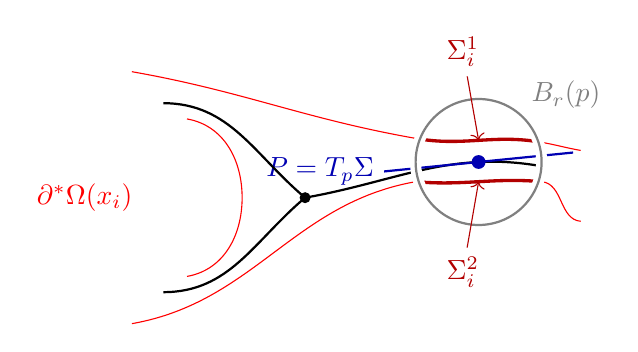
\begin{tikzpicture}[xshift=-0.8cm]
        % Junction point
        \coordinate (J) at (0,0);
        % Long arm: slight upward curve to the right
        \draw[thick] (J) to[out=10, in=170] coordinate[pos=0.75] (P) (3, 0.4);
        % Tangent line at P (blue)
        \draw[thick, bindB] ($(P) + (-1.2, -0.12)$) node[left] {$P = T_p\Sigma$} -- ($(P) + (1.2, 0.12)$);
        % Two short arms going upper-left and lower-left
        \draw[thick] (J) to[out=140, in=0] (-1.8, 1.2);
        \draw[thick] (J) to[out=220, in=0] (-1.8, -1.2);
        % Junction point dot
        \fill (J) circle (2pt);
        % Red sheets — thin bright red (outside circle)
        \draw[thin, red] (-2.2, 1.6) to[out=-10, in=170] ($(P) + (-0.8, 0.3)$) to[out=-10, in=170] ($(P) + (0.8, 0.25)$) to[out=-10, in=170] (3.5, 0.6);
        \draw[thin, red] (-2.2, -1.6) to[out=10, in=190] ($(P) + (-0.8, -0.25)$) to[out=-5, in=175] ($(P) + (0.8, -0.25)$) to[out=-5, in=175] (3.5, -0.3);
        \draw[thin, red] (-1.5, 1.0) to[out=350, in=90] (-0.8, 0) to[out=270, in=10] (-1.5, -1.0);
        % Red sheets — thick (inside circle, clipped)
        \begin{scope}
          \clip (P) circle (0.8);
          \draw[very thick, bindA] (-2.2, 1.6) to[out=-10, in=170] ($(P) + (-0.8, 0.3)$) to[out=-10, in=170] coordinate[pos=0.5] (S1) ($(P) + (0.8, 0.25)$) to[out=-10, in=170] (3.5, 0.6);
          \draw[very thick, bindA] (-2.2, -1.6) to[out=10, in=190] ($(P) + (-0.8, -0.25)$) to[out=-5, in=175] coordinate[pos=0.5] (S2) ($(P) + (0.8, -0.25)$) to[out=-5, in=175] (3.5, -0.3);
        \end{scope}
        % Cut curves at B_r(p) boundary: white eraser then gray circle
        \draw[white, line width=4pt] (P) circle (0.8);
        \draw[gray, thick] (P) circle (0.8);
        \node[gray, above right] at ($(P) + (0.55, 0.55)$) {$B_r(p)$};
        % Blue point on the long arm (drawn on top)
        \fill[bindB] (P) circle (2.5pt);
        % Labels for the two connected components — on top layer
        \node[bindA] (L1) at ($(P) + (-0.2, 1.4)$) {$\Sigma_i^1$};
        \draw[bindA, ->] (L1) -- (S1);
        \node[bindA] (L2) at ($(P) + (-0.2, -1.4)$) {$\Sigma_i^2$};
        \draw[bindA, ->] (L2) -- (S2);
        % Label for all three red curves
        \node[red] at (-2.8, 0) {$\partial^*\Omega(x_i)$};
      \end{tikzpicture}\\[4pt]
      \textbf{(a)}
    \end{minipage}%
    \hfill
    \begin{minipage}[b]{0.38\textwidth}
      \centering
      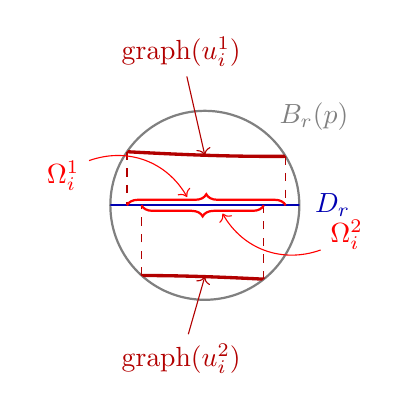
\begin{tikzpicture}[scale=1.5]
        % Define P at origin for this zoomed-in view
        \coordinate (P) at (0,0);
        % Named paths for intersection computation
        \path[name path=circ] (P) circle (0.8);
        \path[name path=sheet1] (-1.5, 0.5) to[out=-3, in=183] (1.5, 0.44);
        \path[name path=sheet2] (-1.5, -0.62) to[out=3, in=177] (1.5, -0.68);
        % Find intersections
        \path[name intersections={of=circ and sheet1, by={I1L,I1R}}];
        \path[name intersections={of=circ and sheet2, by={I2L,I2R}}];
        % Gray circle
        \draw[gray, thick] (P) circle (0.8);
        \node[gray, above right] at ($(P) + (0.55, 0.55)$) {$B_r(p)$};
        % Blue tangent line (clipped to circle) — horizontal
        \begin{scope}
          \clip (P) circle (0.8);
          \draw[thick, bindB] ($(P) + (-1.2, 0)$) -- ($(P) + (1.2, 0)$);
        \end{scope}
        % Two thick red sheets (clipped to circle)
        \begin{scope}
          \clip (P) circle (0.8);
          \draw[very thick, bindA] (-1.5, 0.5) to[out=-3, in=183] coordinate[pos=0.5] (S1b) (1.5, 0.44);
          \draw[very thick, bindA] (-1.5, -0.62) to[out=3, in=177] coordinate[pos=0.5] (S2b) (1.5, -0.68);
        \end{scope}
        % Vertical dashed red lines from exact intersections to D_r
        \draw[thin, bindA, dashed] (I1L) -- (I1L |- P);
        \draw[thin, bindA, dashed] (I1R) -- (I1R |- P);
        \draw[thin, bindA, dashed] (I2L) -- (I2L |- P);
        \draw[thin, bindA, dashed] (I2R) -- (I2R |- P);
        % Braces for domains on D_r
        \draw[red, thick, decorate, decoration={brace, mirror, amplitude=4pt}]
          (I1L |- P) -- (I1R |- P);
        \node[red] (OL2) at (1.2, -0.25) {$\Omega_i^2$};
        \draw[red, thin, ->] (OL2) to[bend left=40] (0.15, -0.07);
        \draw[red, thick, decorate, decoration={brace, amplitude=4pt}]
          (I2R |- P) -- (I2L |- P);
        \node[red] (OL1) at (-1.2, 0.25) {$\Omega_i^1$};
        \draw[red, thin, ->] (OL1) to[bend left=40] (-0.15, 0.07);
        % Labels outside circle with arrows
        \node[bindA] (L1b) at ($(P) + (-0.2, 1.3)$) {$\mathrm{graph}(u_i^1)$};
        \draw[bindA, ->] (L1b) -- (S1b);
        \node[bindA] (L2b) at ($(P) + (-0.2, -1.3)$) {$\mathrm{graph}(u_i^2)$};
        \draw[bindA, ->] (L2b) -- (S2b);
        % Tangent plane label
        \node[bindB, right] at ($(P) + (0.85, 0)$) {$D_r$};
      \end{tikzpicture}\\[4pt]
      \textbf{(b)}
    \end{minipage}
    \caption{Sheet decomposition (Lemma~\ref{lem:sheet-decomposition}) with $\theta(p) = k = 2$. \textbf{(a)}~Near a regular point $p$, the ball $B_r(p)$ cuts the reduced boundary $\partial^*\Omega(x_i)$ into $k = 2$ connected components $\Sigma_i^1, \Sigma_i^2$. \textbf{(b)}~Inside $B_r(p)$: each $\Sigma_i^j = \mathrm{graph}(u_i^j)$ over a domain $\Omega_i^j \subset D_r = P \cap B_r(p)$.}
    \label{fig:sheet-decomposition}
\end{figure}

Before giving the proof, we discuss the geometric content of the three conditions; see Figure~\ref{fig:sheet-decomposition} for an illustration with $k = 2$.

Condition~(i) says that, at sufficiently small scales, $\partial^*\Omega_i \cap B_r(p)$ separates into exactly $k = \theta(p)$ graphical sheets (Figure~\ref{fig:sheet-decomposition}(a)). This is the key step that converts the integer density $\theta(p)$ into a geometric count of sheets.

Condition~(ii) encodes two further properties. The Lipschitz bound $\mathrm{Lip}(u_i^j) < \varepsilon$ controls the \emph{tilt}: each sheet is nearly parallel to the approximate tangent plane $P = T_p\Sigma$, which is the graphical manifestation of small tilt-excess (Definition~\ref{def:p2-tilt-excess}). The coverage bound $\mathcal{H}^n(D_r \setminus \Omega_i^j) < \varepsilon \omega_n r^n$ says that the domain $\Omega_i^j \subset D_r$ covers all but an $\varepsilon$-fraction of the disk $D_r = P \cap B_r(p)$ (Figure~\ref{fig:sheet-decomposition}(b)). Together, the two bounds say that each sheet is a nearly complete, nearly horizontal graph over $D_r$. Figure~\ref{fig:condition-ii} illustrates two configurations that condition~(ii) excludes: a sheet with large tilt (Figure~\ref{fig:condition-ii}(a); which cannot persist as $i \to \infty$, since varifold convergence forces the tilt-excess to decay), and a sheet with poor coverage (Figure~\ref{fig:condition-ii}(b); whose small domain is incompatible with the mass convergence $\|\partial^*\Omega_i\|(B_r(p)) \to \theta(p)\omega_n r^n$).

\begin{figure}[ht]
    \centering
    \begin{minipage}[b]{0.45\textwidth}
      \centering
      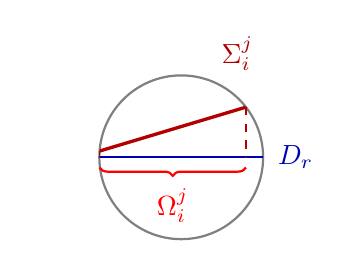
\begin{tikzpicture}[scale=1.3]
        \coordinate (O) at (0,0);
        % Named paths for intersection
        \path[name path=circA] (O) circle (0.8);
        \path[name path=sheetA] (-1.5, -0.15) -- (1.5, 0.75);
        % Gray circle
        \draw[gray, thick] (O) circle (0.8);
        % D_r (blue, horizontal)
        \begin{scope}
          \clip (O) circle (0.8);
          \draw[thick, bindB] (-1.2, 0) -- (1.2, 0);
        \end{scope}
        \node[bindB, right] at (0.85, 0) {$D_r$};
        % Tilted sheet above D_r (large tilt)
        \begin{scope}
          \clip (O) circle (0.8);
          \draw[very thick, bindA] (-1.5, -0.15) -- (1.5, 0.75);
        \end{scope}
        \node[bindA, above right] at (0.3, 0.75) {$\Sigma_i^j$};
        % Intersection points
        \path[name intersections={of=circA and sheetA, by={IAL,IAR}}];
        % Dashed vertical projections to D_r
        \draw[thin, bindA, dashed] (IAL) -- (IAL |- O);
        \draw[thin, bindA, dashed] (IAR) -- (IAR |- O);
        % Coverage domain brace
        \draw[red, thick, decorate, decoration={brace, amplitude=3pt}]
          (IAL |- {(0,-0.1)}) -- (IAR |- {(0,-0.1)}) node[midway, below=4pt, red] {$\Omega_i^j$};
      \end{tikzpicture}\\[4pt]
      \textbf{(a)} Large tilt
    \end{minipage}%
    \hfill
    \begin{minipage}[b]{0.45\textwidth}
      \centering
      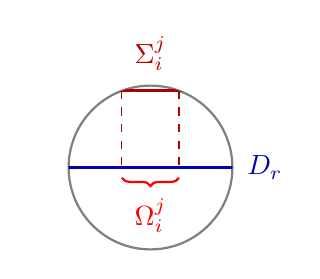
\begin{tikzpicture}[scale=1.3]
        \coordinate (O) at (0,0);
        % Named paths for intersection
        \path[name path=circ] (O) circle (0.8);
        \path[name path=sheet] (-1.2, 0.75) -- (1.2, 0.75);
        % Gray circle
        \draw[gray, thick] (O) circle (0.8);
        % D_r (blue, horizontal)
        \begin{scope}
          \clip (O) circle (0.8);
          \draw[thick, bindB] (-1.2, 0) -- (1.2, 0);
        \end{scope}
        \node[bindB, right] at (0.85, 0) {$D_r$};
        % Short horizontal sheet high above D_r (poor coverage)
        \begin{scope}
          \clip (O) circle (0.8);
          \draw[very thick, bindA] (-1.2, 0.75) -- (1.2, 0.75);
        \end{scope}
        \node[bindA, above] at (0, 0.85) {$\Sigma_i^j$};
        % Intersection points
        \path[name intersections={of=circ and sheet, by={IL,IR}}];
        % Dashed vertical projections to D_r
        \draw[thin, bindA, dashed] (IL) -- (IL |- O);
        \draw[thin, bindA, dashed] (IR) -- (IR |- O);
        % Coverage domain brace
        \draw[red, thick, decorate, decoration={brace, amplitude=3pt}]
          (IL |- {(0,-0.1)}) -- (IR |- {(0,-0.1)}) node[midway, below=4pt, red] {$\Omega_i^j$};
      \end{tikzpicture}\\[4pt]
      \textbf{(b)} Poor coverage
    \end{minipage}
    \caption{Two configurations excluded by condition~(ii) of Lemma~\ref{lem:sheet-decomposition}. In each case the domain $\Omega_i^j$ (brace) is the orthogonal projection of $\Sigma_i^j$ onto $D_r$.}
    \label{fig:condition-ii}
\end{figure}

Condition~(iii) is not independent: it follows from conditions~(i) and~(ii) by the area formula for graphs. Since each sheet $\Sigma_i^j = \mathrm{graph}(u_i^j)$, we have
\[
    \mathcal{H}^n(\Sigma_i^j) = \int_{\Omega_i^j} \sqrt{1 + |Du_i^j|^2} \, d\mathcal{H}^n.
\]
The Lipschitz bound $\mathrm{Lip}(u_i^j) < \varepsilon$ from condition~(ii) gives $\sqrt{1 + |Du_i^j|^2} \in (1, \sqrt{1+\varepsilon^2})$, so
\[
    \mathcal{H}^n(\Omega_i^j) \leq \mathcal{H}^n(\Sigma_i^j) \leq \sqrt{1+\varepsilon^2} \cdot \mathcal{H}^n(\Omega_i^j).
\]
The coverage bound $\mathcal{H}^n(D_r \setminus \Omega_i^j) < \varepsilon\omega_n r^n$ gives $\mathcal{H}^n(\Omega_i^j) \geq (1-\varepsilon)\omega_n r^n$. Combining:
\[
    (1-\varepsilon)\omega_n r^n \leq \mathcal{H}^n(\Sigma_i^j) \leq \sqrt{1+\varepsilon^2} \cdot \omega_n r^n.
\]
For small $\varepsilon$, both sides are close to $\omega_n r^n$, yielding $|\mathcal{H}^n(\Sigma_i^j) - \omega_n r^n| < C\varepsilon \cdot \omega_n r^n$. We include condition~(iii) in the lemma statement for convenience of citation, but it is logically redundant.

We now turn to the proof of Lemma~\ref{lem:sheet-decomposition}.

\begin{proof}
Working in normal coordinates centered at $p$, we identify a neighborhood of $p$ with a neighborhood of the origin in $\mathbb{R}^{n+1}$, the tangent plane $P$ with $\mathbb{R}^n \times \{0\}$, and write $D_r = \{y \in \mathbb{R}^n : |y| < r\}$ for the $n$-disk in $P$. By definition of density (Definition~\ref{def:p2-density}),
\begin{equation}\label{eq:density-ratio-limit}
    \omega_n^{-1} r^{-n} \|V\|(B_r(p)) \to \Theta(\|V\|, p) = \theta(p) \quad \text{as } r \to 0,
\end{equation}
We claim that for any $\varepsilon > 0$, all $r > 0$ sufficiently small, and all $i$ sufficiently large (depending on $r$), the surface $\partial^*\Omega_i \cap B_{2r}(p)$ has mass at most $C\omega_n r^n$ and tilt-excess $E(|\partial^*\Omega_i|, B_{2r}(p), P) < \varepsilon$. The mass bound follows from varifold convergence $|\partial^*\Omega_i| \overset{*}{\rightharpoonup} V$ and~\eqref{eq:density-ratio-limit}. For the tilt-excess: Lemma~\ref{lem:excess-vanishing} gives $E(V, B_{2r}(p), P) \to 0$ as $r \to 0$. Since varifold convergence is weak-$*$ convergence of Radon measures on the Grassmann bundle $M \times G(n+1,n)$, the continuous integrand $|S - P|^2$ yields
\begin{equation}\label{eq:tilt-excess-transfer}
    E(|\partial^*\Omega_i|, B_{2r}(p), P) \to E(V, B_{2r}(p), P) \quad \text{as } i \to \infty
\end{equation}
for a.e.\ $r$ (those satisfying $\|V\|(\partial B_{2r}(p)) = 0$). Choosing first $r$ small, then $i$ large, gives the claim. The surface $\partial^*\Omega_i \cap B_{2r}(p)$ therefore decomposes into finitely many Lipschitz graphs $\Sigma_i^1, \ldots, \Sigma_i^{k_i}$ over $P$ with $\mathrm{Lip}(u_i^j) < C\varepsilon^{1/4}$, plus a non-graphical part of $\mathcal{H}^n$-measure $\leq C\sqrt{\varepsilon}\,r^n$.

It remains to show that each sheet nearly fills $D_r$ (condition~(ii)) and that the sheet count stabilizes (condition~(i)). The strategy is as follows. By the sphere constraint (Step~1), each sheet has height bounded by $r$ and domain containing $D_{r/2}$, giving a crude area lower bound. By the tangent plane condition (Step~2), this crude bound is upgraded to a sharp height estimate $|u_i^j| \leq C\varepsilon^{1/4} r$, which in turn gives sharp coverage $\Omega_i^j \supset D_{r(1-C\varepsilon^{1/2})}$. The sharp coverage is needed for the counting argument: each sheet has area $(1 \pm C\varepsilon)\omega_n r^n$, so $k_i = \theta(p)$.
\medskip\noindent\textbf{Step~1} (Sphere constraint and crude bound). Since $\partial^*\Omega_i$ has no boundary, each graph $\Sigma_i^j$ can only terminate at $\partial B_r(p)$, so every boundary point of the domain $\Omega_i^j$ satisfies $|y|^2 + |u_i^j(y)|^2 = r^2$. Consider a sheet that intersects $B_{r/2}(p)$: there exists a point with $|u_i^j(y_0)| < r/2$, and since $\mathrm{Lip}(u_i^j) < C\varepsilon^{1/4}$, we have $|u_i^j| < r/2 + C\varepsilon^{1/4} r$ on $\Omega_i^j$. Substituting into the sphere constraint, $\Omega_i^j \supset D_{r/2}$ and hence $\mathcal{H}^n(\Omega_i^j) \geq 2^{-n}\omega_n r^n$.

\medskip\noindent\textbf{Step~2} (Tangent plane upgrade). The goal is to show $|u_i^j| \leq C\varepsilon^{1/4} r$ everywhere on each contributing sheet, upgrading the crude bound $|u_i^j| < r$ from Step~1. The key input is that the tangent varifold of $V$ at $p$ is $\theta(p)|P|$, which is supported on $P$. This means that the mass of $V$ far from $P$ is negligible at scale $r$:
\[
    \|V\|(B_r(p) \cap \{\mathrm{dist}(\cdot, P) > \varepsilon^{1/4} r\}) = o(r^n) \quad \text{as } r \to 0.
\]
By varifold convergence, the same holds for $\partial^*\Omega_i$ (for $r$ small, then $i$ large). Since each contributing sheet has area $\geq 2^{-n}\omega_n r^n$ (Step~1) and the total area of $\partial^*\Omega_i \cap B_r(p)$ beyond height $\varepsilon^{1/4} r$ from $P$ is $o(r^n)$, each sheet must contain a point with $|u_i^j| \leq \varepsilon^{1/4} r$. Propagating via $\mathrm{Lip}(u_i^j) < C\varepsilon^{1/4}$ gives $|u_i^j| \leq \varepsilon^{1/4} r + C\varepsilon^{1/4} \cdot 2r \leq C\varepsilon^{1/4} r$ everywhere. The sphere constraint then yields $\Omega_i^j \supset D_{r(1 - C\varepsilon^{1/2})}$, establishing~(ii). Condition~(iii) follows from the area formula for Lipschitz graphs.

\medskip\noindent\textbf{Step~3} (Counting). We count in $B_{r/2}(p)$. Each contributing sheet has domain $\Omega_i^j \supset D_{r/2}$ \textup{(Step~1)} and height $|u_i^j| \leq C\varepsilon^{1/4} r \ll r/2$ \textup{(Step~2)}, so the graph over $D_{r/2}$ lies inside $B_{r/2}(p)$, and the area of each sheet in $B_{r/2}(p)$ satisfies
\[
    (1 - C\varepsilon^{1/2})\omega_n (r/2)^n \leq \mathcal{H}^n(\Sigma_i^j \cap B_{r/2}(p)) \leq (1 + C\varepsilon^{1/2})\omega_n (r/2)^n.
\]
Summing over the $k_i$ sheets, we obtain
\[
    \mathcal{H}^n(\partial^*\Omega_i \cap B_{r/2}(p)) = k_i \,\omega_n (r/2)^n + O(\varepsilon^{1/2})\,(r/2)^n.
\]
Dividing by $\omega_n(r/2)^n$, we get $k_i = \|V\|(B_{r/2}(p)) / (\omega_n(r/2)^n) + O(\varepsilon^{1/2})$. Since $\|V\|(B_{r/2}(p)) / (\omega_n(r/2)^n) \to \theta(p)$ as $r \to 0$ and $k_i \in \mathbb{Z}$, for $r$ and $\varepsilon$ sufficiently small the count $k_i$ equals $\theta(p) \in \mathbb{Z}_{>0}$, establishing~(i).
\end{proof}


\begin{remark}[Role of nestedness]\label{rem:integrality-independence}
The sheet decomposition (Lemma~\ref{lem:sheet-decomposition}) uses nestedness to order the sheets and stabilize the sheet count. The graphical decomposition step (Chebyshev + Caccioppoli $\pi$-injectivity) holds for any sequence of Caccioppoli sets, but nestedness simplifies the integrality conclusion. (Our sheet decomposition is closely related to Wickramasekera's Sheeting Theorem~\cite[Theorem~3.3]{Wic14}, but applies to the \emph{approximating} Caccioppoli boundaries $\partial^*\Omega_i$ rather than the limit, avoiding the need to assume integrality or smoothness a priori.) The $\alpha$-structural verification (Theorem~\ref{thm:alpha-hypo}) uses only the Caccioppoli structure and the min-max width. The non-excessive hypothesis enters in the stability step (Proposition~\ref{prop:stability}), which invokes~\cite[Proposition~3.1]{CLS22}. Nestedness is also used in the parity analysis underlying the multiplicity-one question.
\end{remark}

% !TEX root = ../../main.tex

\section{Regularity}\label{sec:regularity}

By Proposition~\ref{thm:CLS-stationary}, the limit varifold $V$ is stationary; by Theorem~\ref{thm:integrality}, $V$ is integral in the no-mass-cancellation case, and in the mass-cancellation case the integrality of $V$ on $\partial^*\Omega(x_0) \cap \spt\|V\|$ holds unconditionally while integrality on the cancelled mass $\mu_{\mathrm{c}}$ is subject to the gap of Remark~\ref{rem:cancelled-mass-gap}. To promote $V$ to a smooth hypersurface, we apply Wickramasekera's regularity theorem (Theorem~\ref{thm:wickramasekera}), which requires two further inputs---\emph{stability} and the \emph{$\alpha$-structural hypothesis} (Definition~\ref{defn:alpha-structural}). The stability and $\alpha$-structural arguments below apply verbatim to the reduced-boundary part of $V$; under the multiplicity-one conjecture (no mass cancellation), they apply to all of $V$ and yield the full conclusion of Theorem~\ref{thm:non-excessive-main}.

%%%%%%%%%%%%%%%%%%%%%%%%%%%%%%%%%%%%%%%%%%%%%%%%%%%%%%%%%%%%%%%%%%%%%%%%%%%%%%%
\subsection{Stability}\label{subsec:stability}
%%%%%%%%%%%%%%%%%%%%%%%%%%%%%%%%%%%%%%%%%%%%%%%%%%%%%%%%%%%%%%%%%%%%%%%%%%%%%%%

The non-excessive condition provides stability through the following chain of implications: non-excessiveness ensures that the limit varifold $V$ is one-sided homotopic minimizing at all but finitely many points, and one-sided minimization implies stability.

\begin{proposition}[Stability of the limit varifold]\label{prop:stability}
Let $\Phi$ be a non-excessive ONVP sweepout, $x_i \to x_0 \in \mathfrak{m}(\Phi)$ a min-max sequence, and $V$ the varifold limit of $|\partial^*\Omega(x_i)|$. Then $V$ is stable.
\end{proposition}

\begin{proof}
By~\cite[Proposition~3.1]{CLS22}, the set $\mathfrak{h}_{\mathrm{nm}}(V)$ of non-homotopic-minimizing points (Definition~\ref{def:hnm}) is finite. Therefore $V$ is one-sided homotopic minimizing in $B_r(P)$ for every $P \in \spt\|V\| \setminus \mathfrak{h}_{\mathrm{nm}}(V)$ and some $r = r(P) > 0$. One-sided homotopic minimization implies that the second variation $\delta^2 V(\varphi, \varphi) \geq 0$ for all normal deformations $\varphi$ supported in $B_r(P)$. Since the finitely many points of $\mathfrak{h}_{\mathrm{nm}}(V)$ form a set of $\mathcal{H}^n$-measure zero, a partition-of-unity argument extends stability to all compactly supported normal deformations, giving global stability.

We remark that the finiteness of $\mathfrak{h}_{\mathrm{nm}}(V)$ in~\cite[Proposition~3.1]{CLS22} relies on both the non-excessive property and the nestedness of the sweepout: the proof constructs replacement families by ``gluing in'' one-sided homotopies, and nestedness ($\Omega(x_1) \subset \Omega(x_2)$) ensures that the parameter sets on which these replacements are defined are intervals. Nestedness is also used in the integrality argument (see Remark~\ref{rem:integrality-independence}). We also note that~\cite[Proposition~3.1]{CLS22} does not require the identification $V = |\partial^*\Omega(x_0)|$; in particular, the argument applies equally in the mass-cancellation case.
\end{proof}

It remains to verify the $\alpha$-structural hypothesis $(\mathcal{S}3)$. Note that even in the no-mass-cancellation case, where $V = |\partial^*\Omega(x_0)|$ has multiplicity one, the support $\spt\|V\|$ can have singular points where multiple branches meet (e.g., $N = 4$ half-hyperplanes in a balanced configuration); multiplicity one alone does not preclude such junctions. The following verification applies uniformly to both the mass-cancellation and no-mass-cancellation cases.

%%%%%%%%%%%%%%%%%%%%%%%%%%%%%%%%%%%%%%%%%%%%%%%%%%%%%%%%%%%%%%%%%%%%%%%%%%%%%%%
\subsection{The $\alpha$-structural hypothesis}\label{subsec:alpha-structural}
%%%%%%%%%%%%%%%%%%%%%%%%%%%%%%%%%%%%%%%%%%%%%%%%%%%%%%%%%%%%%%%%%%%%%%%%%%%%%%%

\begin{theorem}[Verification of $\alpha$-structural hypothesis]\label{thm:alpha-hypo}
    Let $V$ be the stationary integral varifold arising from a non-excessive ONVP sweepout $\Phi$
    with width $W$, via the min-max sequence $x_i \to x_0 \in \mathfrak{m}(\Phi)$. Then $V$ satisfies the $\alpha$-structural hypothesis (Definition~\ref{defn:alpha-structural}).
\end{theorem}

\begin{proof}
Suppose the $\alpha$-structural hypothesis fails at some $Z \in \sing V$. By definition, $\spt\|V\| \cap B_\rho(Z)$ consists of finitely many $C^{1,\alpha}$ hypersurfaces-with-boundary meeting along a common $C^{1,\alpha}$ boundary $\Gamma$. Blowing up at $Z$, any tangent cone $C$ consists of $N$ half-hyperplanes $P_1^+, \ldots, P_N^+$ meeting along a common edge $L$, with the stationarity balance $\sum_{j=1}^N m_j \nu_j = 0$. By Remark~\ref{rem:S-alpha-remarks}(ii), $N \geq 3$, so the pigeonhole principle gives two adjacent half-hyperplanes $P_j^+, P_{j+1}^+$ meeting at angle $\theta_j \leq 2\pi/N < \pi$.

\medskip\noindent\textbf{Step~1: Chord-beats-arc on the tangent cone.}
In each two-dimensional cross-section normal to $L$, the two half-lines $P_j^+ \cap \partial B_r$ and $P_{j+1}^+ \cap \partial B_r$ have total length $2r$, while the chord connecting their endpoints has length $2r\sin(\theta_j/2) < 2r$ (see Figure~\ref{fig:chord-beats-arc}). Integrating along $L$, the replacement surface has strictly less area:
\[
    \|C\|(B_r) - \|\widetilde{C}\|(B_r) \geq \delta(\theta_j) \cdot r^n > 0.
\]

    \begin{figure}[ht]
        \centering
        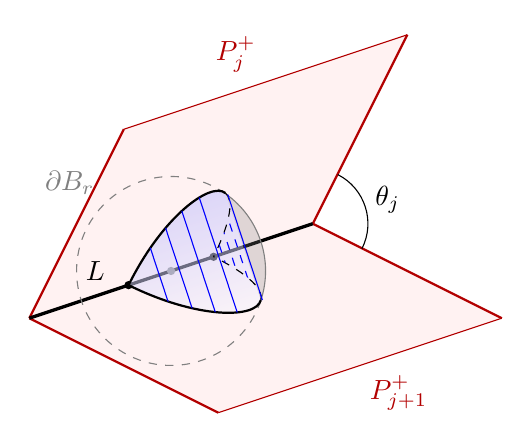
\begin{tikzpicture}[scale=1.0]
          % Edge L: shared edge of the two parallelograms, with perspective
          \coordinate (A) at (-1.8,-0.6);   % near end of edge
          \coordinate (B) at (1.8,0.6);     % far end of edge

          % H_1 (upper half-plane): parallelogram above L
          \coordinate (A1) at ($(A)+(1.2,2.4)$);
          \coordinate (B1) at ($(B)+(1.2,2.4)$);

          % H_2 (lower half-plane): parallelogram below L
          \coordinate (A2) at ($(A)+(2.4,-1.2)$);
          \coordinate (B2) at ($(B)+(2.4,-1.2)$);

          % Fill both half-planes
          \fill[fillA, opacity=0.35] (A) -- (B) -- (B1) -- (A1) -- cycle;
          \fill[fillA, opacity=0.35] (A) -- (B) -- (B2) -- (A2) -- cycle;

          % Draw H_1 edges
          \draw[thick, bindA] (A) -- (A1);
          \draw[thick, bindA] (B) -- (B1);
          \draw[bindA] (A1) -- (B1);

          % Draw H_2 edges
          \draw[thick, bindA] (A) -- (A2);
          \draw[thick, bindA] (B) -- (B2);
          \draw[bindA] (A2) -- (B2);

          % Edge L (drawn on top)
          \draw[very thick] (A) -- (B);

          % Midpoint of L and ball B_r
          \coordinate (M) at ($(A)!0.5!(B)$);
          % Circle split at tangent points: short arc (right) solid, long arc (left) dashed
          \draw[gray, thin] ($(M)+(-18:1.2)$) arc[start angle=-18, end angle=55, radius=1.2];
          \draw[gray, thin, dashed] ($(M)+(55:1.2)$) arc[start angle=55, end angle=342, radius=1.2];
          \fill[gray] (M) circle (1.5pt);
          \node[gray, above left] at ($(M)+(135:1.2)$) {$\partial B_r$};

          % Two points on L inside the circle, on either side of M
          \coordinate (P) at ($(A)!0.35!(B)$);
          \coordinate (Q) at ($(A)!0.65!(B)$);
          \fill (P) circle (1.5pt);
          \fill (Q) circle (1.5pt);

          % Blue gradient shading for chord competitor (between semi-ellipses and chord)
          \shade[left color=blue!30, right color=blue!5, shading angle=18, opacity=0.5]
            (P) .. controls (-0.11, 0.69) and (0.50, 1.14) .. (0.69, 0.99)
            -- (1.14, -0.37)
            .. controls (1.08, -0.61) and (0.33, -0.61) .. cycle;

          % Gray shading for the wedge region (between chord and arc)
          \fill[gray, opacity=0.25]
            (0.69, 0.99) -- (1.14, -0.37)
            arc[start angle=-18, end angle=55, radius=1.2]
            -- cycle;

          % Semi-ellipse on H_1 side: solid left part, dashed right part
          \draw[thick] (P) .. controls (-0.11, 0.69) and (0.50, 1.14) .. (0.69, 0.99);
          \draw[thin, dashed] (0.69, 0.99) .. controls (0.79, 0.91) and (0.77, 0.65) .. (Q);

          % Semi-ellipse on H_2 side: solid left part, dashed right part
          \draw[thick] (P) .. controls (0.33, -0.61) and (1.08, -0.61) .. (1.14, -0.37);
          \draw[thin, dashed] (1.14, -0.37) .. controls (1.18, -0.25) and (1.01, -0.05) .. (Q);

          % Chord competitor: sparse parallel blue lines clipped to competitor region
          \begin{scope}
            \clip (P) .. controls (-0.11, 0.69) and (0.50, 1.14) .. (0.69, 0.99)
              -- (1.14, -0.37)
              .. controls (1.08, -0.61) and (0.33, -0.61) .. cycle;
            \foreach \s in {-0.15, 0.1, 0.35, 0.6} {
              \draw[blue, thin] ({\s-0.9}, {\s/3+2.72}) -- ({\s+0.9}, {\s/3-2.72});
            }
          \end{scope}

          % Rightmost solid blue line: shifted slightly right of T1-T2 to cover dashed ellipses
          \draw[blue, thin] (0.72, 0.97) -- (1.16, -0.37);

          % Past tangent points: dense dashed blue lines in the wedge region
          \begin{scope}
            \clip ($(M)+(-18:1.2)$)
              arc[start angle=-18, end angle=55, radius=1.2]
              .. controls (0.79, 0.91) and (0.77, 0.65) .. (Q)
              .. controls (1.01, -0.05) and (1.18, -0.25) .. cycle;
            \foreach \s in {-0.45,-0.35,...,0.85} {
              \draw[blue, thin, dashed] ({\s-0.9}, {\s/3+2.72}) -- ({\s+0.9}, {\s/3-2.72});
            }
          \end{scope}

          % Angle arc at far end B (interior angle, the Omega_C side)
          \draw[thin] (B) ++(-27:0.7) arc[start angle=-27, end angle=63, radius=0.7];
          \node at ($(B)+(18:1.0)$) {$\theta_j$};

          % Labels
          \node[bindA, above left] at ($(A1)!0.5!(B1)$) {$P_j^+$};
          \node[bindA, below right] at ($(A2)!0.5!(B2)$) {$P_{j+1}^+$};
          \node[above left] at ($(A)!0.3!(B)$) {$L$};
        \end{tikzpicture}
        \caption{Chord-beats-arc: two adjacent half-hyperplanes $P_j^+, P_{j+1}^+$ meet along the $(n-1)$-dimensional edge $L$ at angle $\theta_j < \pi$ (by the balancing condition and pigeonhole, Remark~\ref{rem:S-alpha-remarks}(ii)). In each $2$-dimensional cross-section normal to $L$, the two half-lines (solid arcs on the shaded half-planes) have total length $2r$, while the chord (blue hatched surface) has length $2r\sin(\theta_j/2) < 2r$. The grey region is the area saved by the replacement.}
        \label{fig:chord-beats-arc}
    \end{figure}

\medskip\noindent\textbf{Step~2: Transfer to $B_r(Z)$ and the approximating sequence.}
We transfer the cone-level area deficit to the approximating Caccioppoli sets. Choose normal coordinates centered at $Z$ so that $g_{ij}(Z) = \delta_{ij}$; then $g_{ij} = \delta_{ij} + O(r)$ in $B_r(Z)$. Since the $\alpha$-structural hypothesis fails at~$Z$, the $C^{1,\alpha}$ branches of $\spt\|V\|$ in $B_\rho(Z)$ converge to the tangent cone under blow-up: at scale~$r$, each branch deviates from its limiting half-hyperplane by $O(r^{1+\alpha})$, and the angle between adjacent branches is $\theta_j + O(r^\alpha)$, which remains $< \pi$ for $r$ sufficiently small.

By varifold convergence $|\partial^*\Omega(x_i)| \to V$ and the sheet decomposition (Lemma~\ref{lem:sheet-decomposition}), for each $r \in (0, \rho)$ sufficiently small and all $i$ sufficiently large, the smooth boundary $\partial^*\Omega(x_i) \cap B_r(Z)$ decomposes into smooth sheets, each a nearly flat graph approximating one of the $C^{1,\alpha}$ branches of $\spt\|V\|$. In particular, two adjacent sheets approximate $P_j^+$ and $P_{j+1}^+$, meeting at angle $\theta_j + O(r^\alpha) < \pi$ in $B_r(Z)$.
\begin{figure}[ht]
    \centering
    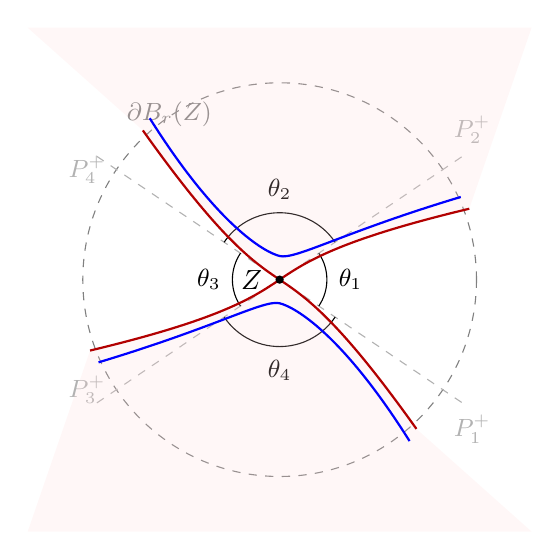
\begin{tikzpicture}[scale=1.0]
      % Ball B_r(Z)
      \draw[gray, thin, dashed] (0,0) circle (2.5);
      \node[gray] at (-1.4, 2.1) {\small $\partial B_r(Z)$};

      % Tangent angle at Z for each curve
      \pgfmathsetmacro{\tA}{34}   % curve 1 tangent angle
      \pgfmathsetmacro{\tB}{-34}  % curve 2 tangent angle

      % Tangent lines at Z (gray dashed) — exact directions from \tA, \tB
      \draw[gray!60, dashed, thin] ({-2.8*cos(\tA)}, {-2.8*sin(\tA)}) -- ({2.8*cos(\tA)}, {2.8*sin(\tA)});
      \draw[gray!60, dashed, thin] ({-2.8*cos(\tB)}, {-2.8*sin(\tB)}) -- ({2.8*cos(\tB)}, {2.8*sin(\tB)});

      % Labels for P_1^+ through P_4^+ (four half-lines = rays from Z)
      \node[gray!60] at ({2.95*cos(\tB)}, {2.95*sin(\tB)-0.25}) {\small $P_1^+$};
      \node[gray!60] at ({2.95*cos(\tA)}, {2.95*sin(\tA)+0.25}) {\small $P_2^+$};
      \node[gray!60] at ({-2.95*cos(\tA)}, {-2.95*sin(\tA)+0.25}) {\small $P_3^+$};
      \node[gray!60] at ({-2.95*cos(\tB)}, {-2.95*sin(\tB)-0.25}) {\small $P_4^+$};

      % θ_1: P_1 (-34°) to P_2 (34°) — narrow angle, upper wedge
      \draw[thin] ({0.6*cos(\tB)}, {0.6*sin(\tB)}) arc[start angle=\tB, end angle=\tA, radius=0.6];
      \node at ({0.9*cos(0)}, {0.9*sin(0)}) {\small $\theta_1$};

      % θ_2: P_2 (34°) to P_3 (146°) — wide angle, left
      \draw[thin] ({0.85*cos(\tA)}, {0.85*sin(\tA)}) arc[start angle=\tA, end angle={180+\tB}, radius=0.85];
      \node at ({1.15*cos(90)}, {1.15*sin(90)}) {\small $\theta_2$};

      % θ_3: P_3 (146°) to P_4 (214°) — narrow angle, lower wedge
      \draw[thin] ({0.6*cos(180+\tB)}, {0.6*sin(180+\tB)}) arc[start angle={180+\tB}, end angle={180+\tA}, radius=0.6];
      \node at ({0.9*cos(180)}, {0.9*sin(180)}) {\small $\theta_3$};

      % θ_4: P_4 (214°) to P_1 (326°) — wide angle, right
      \draw[thin] ({0.85*cos(180+\tA)}, {0.85*sin(180+\tA)}) arc[start angle={180+\tA}, end angle={360+\tB}, radius=0.85];
      \node at ({1.15*cos(270)}, {1.15*sin(270)}) {\small $\theta_4$};

      % Upper shaded region (between curve 1 right branch and curve 2 left branch)
      \begin{scope}
      \clip (-3.2,-3.2) rectangle (3.2,3.2);
      \fill[fillA, opacity=0.2]
        (0,0)
        .. controls ({0.4*cos(\tA)}, {0.4*sin(\tA)}) and ({0.9*cos(\tA)}, {0.9*sin(\tA)}) ..
        ({2.5*cos(\tA)+0.6*sin(\tA)}, {2.5*sin(\tA)-0.6*cos(\tA)})
        -- (3.2, 3.2) -- (-3.2, 3.2)
        -- ({-2.5*cos(\tB)-0.6*sin(\tB)}, {-2.5*sin(\tB)+0.6*cos(\tB)})
        .. controls ({-0.9*cos(\tB)}, {-0.9*sin(\tB)}) and ({-0.4*cos(\tB)}, {-0.4*sin(\tB)}) ..
        (0,0);
      \end{scope}

      % Lower shaded region (between curve 2 right branch and curve 1 left branch)
      \begin{scope}
      \clip (-3.2,-3.2) rectangle (3.2,3.2);
      \fill[fillA, opacity=0.2]
        (0,0)
        .. controls ({0.4*cos(\tB)}, {0.4*sin(\tB)}) and ({0.9*cos(\tB)}, {0.9*sin(\tB)}) ..
        ({2.5*cos(\tB)+0.6*sin(\tB)}, {2.5*sin(\tB)-0.6*cos(\tB)})
        -- (3.2, -3.2) -- (-3.2, -3.2)
        -- ({-2.5*cos(\tA)-0.6*sin(\tA)}, {-2.5*sin(\tA)+0.6*cos(\tA)})
        .. controls ({-0.9*cos(\tA)}, {-0.9*sin(\tA)}) and ({-0.4*cos(\tA)}, {-0.4*sin(\tA)}) ..
        (0,0);
      \end{scope}

      % Curve 1: control points near Z lie on tangent direction \tA
      \draw[bindA, thick]
        ({-2.5*cos(\tA) - 0.6*sin(\tA)}, {-2.5*sin(\tA) + 0.6*cos(\tA)})
        .. controls ({-0.9*cos(\tA)}, {-0.9*sin(\tA)}) and ({-0.4*cos(\tA)}, {-0.4*sin(\tA)}) .. (0,0)
        .. controls ({0.4*cos(\tA)}, {0.4*sin(\tA)}) and ({0.9*cos(\tA)}, {0.9*sin(\tA)}) ..
        ({2.5*cos(\tA) + 0.6*sin(\tA)}, {2.5*sin(\tA) - 0.6*cos(\tA)});

      % Curve 2: control points near Z lie on tangent direction \tB
      \draw[bindA, thick]
        ({-2.5*cos(\tB) - 0.6*sin(\tB)}, {-2.5*sin(\tB) + 0.6*cos(\tB)})
        .. controls ({-0.9*cos(\tB)}, {-0.9*sin(\tB)}) and ({-0.4*cos(\tB)}, {-0.4*sin(\tB)}) .. (0,0)
        .. controls ({0.4*cos(\tB)}, {0.4*sin(\tB)}) and ({0.9*cos(\tB)}, {0.9*sin(\tB)}) ..
        ({2.5*cos(\tB) + 0.6*sin(\tB)}, {2.5*sin(\tB) - 0.6*cos(\tB)});

      % Blue curve (∂*Ω_i sheet) in upper wedge, just above the red boundary
      \draw[blue, thick]
        (-1.65, 2.05) .. controls (-0.8, 0.7) and (-0.2, 0.35) .. (0, 0.3)
        .. controls (0.2, 0.25) and (0.8, 0.6) .. (2.3, 1.05);

      % Blue curve (∂*Ω_i sheet) in lower wedge, rotated 180° from the upper one
      \draw[blue, thick]
        (1.65, -2.05) .. controls (0.8, -0.7) and (0.2, -0.35) .. (0, -0.3)
        .. controls (-0.2, -0.25) and (-0.8, -0.6) .. (-2.3, -1.05);

      % Point Z
      \fill (0,0) circle (1.5pt);
      \node[left] at (-0.1, 0) {$Z$};
    \end{tikzpicture}
    \caption{Cross-section normal to $L$ at $Z$: the tangent cone half-lines $P_j^+, P_{j+1}^+$ (gray dashed) and the $C^{1,\alpha}$ branches of $\spt\|V\|$ (red solid). The branches deviate from the half-lines by $O(r^{1+\alpha})$; the angle between adjacent branches is $\theta_j + O(r^\alpha) < \pi$.}
    \label{fig:transfer}
\end{figure}

\medskip\noindent\textbf{Step~3: Caccioppoli surgery and contradiction with width.}
We perform chord surgery on the approximating Caccioppoli sets. In $B_r(Z)$, the two smooth sheets of $\partial^*\Omega(x_i)$ corresponding to the narrowest adjacent pair bound a thin wedge-shaped region. Replace these two sheets inside $B_{r/2}(Z)$ by a smooth interpolation surface (the ``chord surface''), which spans the same boundary on $\partial B_{r/2}(Z)$ but cuts across the wedge.
\begin{figure}[ht]
    \centering
    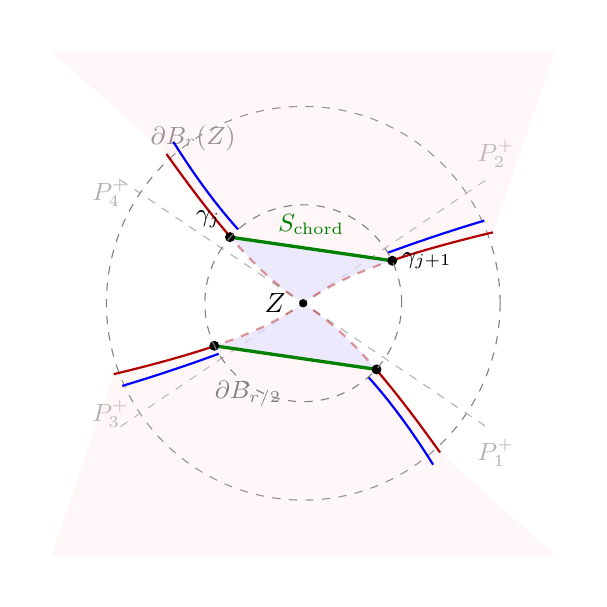
\begin{tikzpicture}[scale=1.0]
      % Ball B_r(Z)
      \draw[gray, thin, dashed] (0,0) circle (2.5);
      \node[gray] at (-1.4, 2.1) {\small $\partial B_r(Z)$};

      % Tangent angle at Z for each curve
      \pgfmathsetmacro{\tA}{34}   % curve 1 tangent angle
      \pgfmathsetmacro{\tB}{-34}  % curve 2 tangent angle

      % Tangent lines at Z (gray dashed) — exact directions from \tA, \tB
      \draw[gray!60, dashed, thin] ({-2.8*cos(\tA)}, {-2.8*sin(\tA)}) -- ({2.8*cos(\tA)}, {2.8*sin(\tA)});
      \draw[gray!60, dashed, thin] ({-2.8*cos(\tB)}, {-2.8*sin(\tB)}) -- ({2.8*cos(\tB)}, {2.8*sin(\tB)});

      % Labels for P_1^+ through P_4^+ (four half-lines = rays from Z)
      \node[gray!60] at ({2.95*cos(\tB)}, {2.95*sin(\tB)-0.25}) {\small $P_1^+$};
      \node[gray!60] at ({2.95*cos(\tA)}, {2.95*sin(\tA)+0.25}) {\small $P_2^+$};
      \node[gray!60] at ({-2.95*cos(\tA)}, {-2.95*sin(\tA)+0.25}) {\small $P_3^+$};
      \node[gray!60] at ({-2.95*cos(\tB)}, {-2.95*sin(\tB)-0.25}) {\small $P_4^+$};

      % Upper shaded region (between curve 1 right branch and curve 2 left branch)
      \begin{scope}
      \clip (-3.2,-3.2) rectangle (3.2,3.2);
      \fill[fillA, opacity=0.2]
        (0,0)
        .. controls ({0.4*cos(\tA)}, {0.4*sin(\tA)}) and ({0.9*cos(\tA)}, {0.9*sin(\tA)}) ..
        ({2.5*cos(\tA)+0.6*sin(\tA)}, {2.5*sin(\tA)-0.6*cos(\tA)})
        -- (3.2, 3.2) -- (-3.2, 3.2)
        -- ({-2.5*cos(\tB)-0.6*sin(\tB)}, {-2.5*sin(\tB)+0.6*cos(\tB)})
        .. controls ({-0.9*cos(\tB)}, {-0.9*sin(\tB)}) and ({-0.4*cos(\tB)}, {-0.4*sin(\tB)}) ..
        (0,0);
      \end{scope}

      % Lower shaded region (between curve 2 right branch and curve 1 left branch)
      \begin{scope}
      \clip (-3.2,-3.2) rectangle (3.2,3.2);
      \fill[fillA, opacity=0.2]
        (0,0)
        .. controls ({0.4*cos(\tB)}, {0.4*sin(\tB)}) and ({0.9*cos(\tB)}, {0.9*sin(\tB)}) ..
        ({2.5*cos(\tB)+0.6*sin(\tB)}, {2.5*sin(\tB)-0.6*cos(\tB)})
        -- (3.2, -3.2) -- (-3.2, -3.2)
        -- ({-2.5*cos(\tA)-0.6*sin(\tA)}, {-2.5*sin(\tA)+0.6*cos(\tA)})
        .. controls ({-0.9*cos(\tA)}, {-0.9*sin(\tA)}) and ({-0.4*cos(\tA)}, {-0.4*sin(\tA)}) ..
        (0,0);
      \end{scope}

      % Red curves OUTSIDE B_{r/2} (solid — retained)
      \begin{scope}
        \pgfseteorule\clip (-3.5,-3.5) rectangle (3.5,3.5) (0,0) circle (1.25);
        \draw[bindA, thick]
          ({-2.5*cos(\tA) - 0.6*sin(\tA)}, {-2.5*sin(\tA) + 0.6*cos(\tA)})
          .. controls ({-0.9*cos(\tA)}, {-0.9*sin(\tA)}) and ({-0.4*cos(\tA)}, {-0.4*sin(\tA)}) .. (0,0)
          .. controls ({0.4*cos(\tA)}, {0.4*sin(\tA)}) and ({0.9*cos(\tA)}, {0.9*sin(\tA)}) ..
          ({2.5*cos(\tA) + 0.6*sin(\tA)}, {2.5*sin(\tA) - 0.6*cos(\tA)});
        \draw[bindA, thick]
          ({-2.5*cos(\tB) - 0.6*sin(\tB)}, {-2.5*sin(\tB) + 0.6*cos(\tB)})
          .. controls ({-0.9*cos(\tB)}, {-0.9*sin(\tB)}) and ({-0.4*cos(\tB)}, {-0.4*sin(\tB)}) .. (0,0)
          .. controls ({0.4*cos(\tB)}, {0.4*sin(\tB)}) and ({0.9*cos(\tB)}, {0.9*sin(\tB)}) ..
          ({2.5*cos(\tB) + 0.6*sin(\tB)}, {2.5*sin(\tB) - 0.6*cos(\tB)});
      \end{scope}

      % Intersection points of RED curves with ∂B_{r/2}
      % Upper wedge: right branch of curve 1 (P_2^+) and left branch of curve 2 (toward P_3^+)
      \coordinate (UR) at (1.13, 0.54);    % curve 1 right branch ∩ ∂B_{r/2}
      \coordinate (UL) at (-0.93, 0.84);   % curve 2 left branch ∩ ∂B_{r/2}
      % Lower wedge: left branch of curve 1 (P_4^+) and right branch of curve 2 (toward P_1^+)
      \coordinate (LL) at (-1.13, -0.54);  % curve 1 left branch ∩ ∂B_{r/2}
      \coordinate (LR) at (0.93, -0.84);   % curve 2 right branch ∩ ∂B_{r/2}

      % Saved area in upper wedge (between red curves and chord, inside B_{r/2})
      \begin{scope}
        \clip (0,0) circle (1.25);
        \fill[blue!12, opacity=0.6]
          (0,0)
          .. controls (0.22, 0.15) and (0.48, 0.33) .. (UR)
          -- (UL)
          .. controls (-0.48, 0.33) and (-0.22, 0.15) .. (0,0);
      \end{scope}

      % Saved area in lower wedge
      \begin{scope}
        \clip (0,0) circle (1.25);
        \fill[blue!12, opacity=0.6]
          (0,0)
          .. controls (-0.22, -0.15) and (-0.48, -0.33) .. (LL)
          -- (LR)
          .. controls (0.48, -0.33) and (0.22, -0.15) .. (0,0);
      \end{scope}

      % Blue curves (∂*Ω(x) sheets) — OUTSIDE B_{r/2} only (solid)
      \begin{scope}
        \pgfseteorule\clip (-3.5,-3.5) rectangle (3.5,3.5) (0,0) circle (1.25);
        \draw[blue, thick]
          (-1.65, 2.05) .. controls (-0.8, 0.7) and (-0.2, 0.35) .. (0, 0.3)
          .. controls (0.2, 0.25) and (0.8, 0.6) .. (2.3, 1.05);
        \draw[blue, thick]
          (1.65, -2.05) .. controls (0.8, -0.7) and (0.2, -0.35) .. (0, -0.3)
          .. controls (-0.2, -0.25) and (-0.8, -0.6) .. (-2.3, -1.05);
      \end{scope}

      % Red curves INSIDE B_{r/2} — dashed (replaced by chord surgery)
      \begin{scope}
        \clip (0,0) circle (1.25);
        \draw[bindA, thick, dashed, opacity=0.4]
          ({-2.5*cos(\tA) - 0.6*sin(\tA)}, {-2.5*sin(\tA) + 0.6*cos(\tA)})
          .. controls ({-0.9*cos(\tA)}, {-0.9*sin(\tA)}) and ({-0.4*cos(\tA)}, {-0.4*sin(\tA)}) .. (0,0)
          .. controls ({0.4*cos(\tA)}, {0.4*sin(\tA)}) and ({0.9*cos(\tA)}, {0.9*sin(\tA)}) ..
          ({2.5*cos(\tA) + 0.6*sin(\tA)}, {2.5*sin(\tA) - 0.6*cos(\tA)});
        \draw[bindA, thick, dashed, opacity=0.4]
          ({-2.5*cos(\tB) - 0.6*sin(\tB)}, {-2.5*sin(\tB) + 0.6*cos(\tB)})
          .. controls ({-0.9*cos(\tB)}, {-0.9*sin(\tB)}) and ({-0.4*cos(\tB)}, {-0.4*sin(\tB)}) .. (0,0)
          .. controls ({0.4*cos(\tB)}, {0.4*sin(\tB)}) and ({0.9*cos(\tB)}, {0.9*sin(\tB)}) ..
          ({2.5*cos(\tB) + 0.6*sin(\tB)}, {2.5*sin(\tB) - 0.6*cos(\tB)});
      \end{scope}

      % Chord surfaces S_chord (green, connecting red-curve traces on ∂B_{r/2})
      \draw[green!50!black, very thick] (UL) -- (UR);
      \draw[green!50!black, very thick] (LR) -- (LL);

      % Intersection points γ_j, γ_{j+1} on ∂B_{r/2}
      \fill (UL) circle (1.8pt);
      \fill (UR) circle (1.8pt);
      \fill (LR) circle (1.8pt);
      \fill (LL) circle (1.8pt);

      % Labels
      \node[above left, font=\small] at (UL) {$\gamma_j$};
      \node[right, font=\small] at (UR) {$\gamma_{j+1}$};
      \node[green!50!black, above, font=\small] at (0.1, 0.75) {$S_{\mathrm{chord}}$};

      % Inner ball B_{r/2}(Z)
      \draw[gray, thin, dashed] (0,0) circle (1.25);
      \node[gray] at (-0.7, -1.15) {\small $\partial B_{r/2}$};

      % Point Z
      \fill (0,0) circle (1.5pt);
      \node[left] at (-0.1, 0) {$Z$};
    \end{tikzpicture}
    \caption{Chord surgery (cross-section normal to $L$). The sheets of $\partial^*\Omega(x)$ (blue solid) approximate the $C^{1,\alpha}$ branches of $\spt\|V\|$ (red) in the narrow wedge regions. Inside $B_{r/2}(Z)$ (inner dashed circle), the original sheets (blue dashed) are replaced by chord surfaces $S_{\mathrm{chord}}$ (green), connecting the traces $\gamma_j, \gamma_{j+1}$ on $\partial B_{r/2}(Z)$. The shaded region is the area saved by the surgery: $\geq \delta(\theta_j) r^n / 2 > 0$.}
    \label{fig:surgery}
\end{figure}

\noindent\textbf{Step~3a: Chord surgery on a single slice.}
Let $\Sigma_j(x)$ and $\Sigma_{j+1}(x)$ denote the two adjacent sheets of $\partial^*\Omega(x)$ in $B_r(Z)$ approximating $P_j^+$ and $P_{j+1}^+$. Work in normal coordinates centered at $Z$ and decompose $\mathbb{R}^{n+1} = L \oplus L^\perp$, where $L$ is the $(n-1)$-dimensional edge of the tangent cone. For $\rho \in (0, r/2]$ and $y \in L$ with $|y| < \rho$, let $\Pi_y := \{y\} + L^\perp$ be the $2$-dimensional affine plane through $y$ perpendicular to $L$. Each sheet $\Sigma_k(x)$ ($k = j, j+1$) intersects the circle $\partial B_\rho(Z) \cap \Pi_y$ transversally at a point $p_k(y,x)$ on the narrow-wedge side. Define the \emph{chord surface at scale~$\rho$} as the ruled surface
\[
    S_{\mathrm{chord}}^{\rho}(x) \;:=\; \big\{(1-t)\, p_j(y,x) + t\, p_{j+1}(y,x) \,:\, y \in L \cap B_{\rho}(Z),\; t \in [0,1]\big\},
\]
i.e., in each cross-section $\Pi_y$ the two sheet-arcs inside $B_\rho(Z)$ are replaced by the straight segment connecting their trace points on $\partial B_\rho(Z)$. Let $T_{\rho}(x) \subset B_{\rho}(Z)$ denote the open region bounded by $\Sigma_j(x) \cap B_{\rho}(Z)$, $\Sigma_{j+1}(x) \cap B_{\rho}(Z)$, and $S_{\mathrm{chord}}^{\rho}(x)$---the \emph{wedge tip} cut off by the chord (see Figure~\ref{fig:surgery}). The surgered set is
\[
    \Omega(x)_\rho \;:=\; \Omega(x) \,\triangle\, T_\rho(x).
\]
Since $T_\rho(x) \subset B_\rho(Z)$, the set $\Omega(x)_\rho$ agrees with $\Omega(x)$ outside $B_\rho(Z)$, and inside $B_\rho(Z)$ the two sheets $\Sigma_j(x), \Sigma_{j+1}(x)$ are replaced by the single chord surface $S_{\mathrm{chord}}^{\rho}(x)$. The symmetric difference formulation handles both possible orientations of the wedge (whether $T_\rho(x) \subset \Omega(x)$ or $T_\rho(x) \subset M \setminus \Omega(x)$) uniformly.

In each cross-section $\Pi_y$, the chord segment $\overline{p_j\, p_{j+1}}$ has length $2\rho_y\sin(\theta_j/2)$, strictly less than the total length $2\rho_y$ of the two sheet-arcs it replaces (where $\rho_y = \sqrt{\rho^2 - |y|^2}$). Integrating along $L$ and accounting for the $C^{1,\alpha}$ deviation of the sheets and the $O(\rho)$ metric distortion:
\[
    \mathrm{Per}(\Omega(x)_\rho) \leq \mathrm{Per}(\Omega(x)) - \frac{\delta(\theta_j)}{2}\, \rho^n,
\]
where $\delta(\theta_j) > 0$ depends only on $\theta_j$ and $n$. The constant $\delta(\theta_j)$ and the radius $r$ depend on the tangent cone geometry at $Z$---the $C^{1,\alpha}$ branches of $\spt\|V\|$---but not on the individual slice; the saving is therefore uniform over all slices whose boundary decomposes into the same sheet structure.

\medskip\noindent\textbf{Step~3b: Uniformity over nearby slices.}
By continuity of $\Phi$ in the flat topology, there exists $\varepsilon > 0$ such that for every $x$ with $|x - x_0| < \varepsilon$, the boundary $\partial^*\Omega(x) \cap B_r(Z)$ admits the same sheet decomposition as described in Step~3a. The chord surgery at any scale $\rho \leq r/2$ then saves at least $\delta(\theta_j)\rho^n/2 > 0$ uniformly for all such $x$.

\medskip\noindent\textbf{Step~3c: Modified sweepout with $\mathcal{F}$-continuity.}
A na\"ive piecewise definition---performing the full surgery for $|x - x_0| < \varepsilon$ and no surgery otherwise---fails to be $\mathcal{F}$-continuous at $|x - x_0| = \varepsilon$, since the surgery modifies $\Omega(x)$ by a fixed positive volume inside $B_{r/2}(Z)$.

To ensure continuity, we use a \emph{shrinking surgery ball}. Let $\eta \colon [0,\infty) \to [0,1]$ be a smooth non-increasing function with $\eta \equiv 1$ on $[0, \tfrac{1}{2}]$ and $\eta \equiv 0$ on $[1, \infty)$. Define the \emph{shrinking surgery radius} $\rho(x) := (r/2)\cdot\eta(|x - x_0|/\varepsilon)$, so that $\rho(x) = r/2$ for $|x - x_0| \leq \varepsilon/2$ and $\rho(x) = 0$ for $|x - x_0| \geq \varepsilon$. The chord surgery at scale $\rho(x)$ is well defined whenever $\rho(x) > 0$ (the sheet decomposition holds at every scale $\leq r/2$). Set
\[
    \tilde{\Omega}(x) \;:=\; \Omega(x) \,\triangle\, T_{\rho(x)}(x),
\]
with the convention $T_0(x) := \varnothing$. Thus $\tilde{\Omega}(x) = \Omega(x)$ for $|x - x_0| \geq \varepsilon$, and $\tilde{\Omega}(x) = \Omega(x)_{r/2}$ for $|x - x_0| \leq \varepsilon/2$.

We verify that $\tilde{\Phi}(x) := \partial\tilde{\Omega}(x)$ is $\mathcal{F}$-continuous. By the triangle inequality for the flat metric,
\[
    \mathrm{Vol}\big(\tilde{\Omega}(x) \,\triangle\, \tilde{\Omega}(y)\big)
    \;\leq\; \mathrm{Vol}\big(\Omega(x) \,\triangle\, \Omega(y)\big)
    \;+\; \mathrm{Vol}\big(T_{\rho(x)}(x) \,\triangle\, T_{\rho(y)}(y)\big).
\]
The first term tends to zero as $y \to x$ by $\mathcal{F}$-continuity of $\Phi$. For the second term, note that $T_\rho(x)$ depends on $x$ through the sheets $\Sigma_j(x)$, $\Sigma_{j+1}(x)$ and the scale $\rho(x)$. As $y \to x$: the scale $\rho(y) \to \rho(x)$ by smoothness of $\eta$; and the sheets converge in $C^1(B_r(Z))$, since flat convergence $\Omega(y) \to \Omega(x)$ combined with the uniform perimeter bound (all slices have $\mathrm{Per} \leq W + 1$) implies varifold convergence of boundaries, which for graphical sheets with small $C^{1,\alpha}$ norm over the tangent half-hyperplanes upgrades to smooth convergence by standard graphical estimates~\cite[Theorem~24.2]{Sim84}. Therefore $\mathrm{Vol}(T_{\rho(x)}(x) \,\triangle\, T_{\rho(y)}(y)) \to 0$, and $\tilde{\Phi}$ is $\mathcal{F}$-continuous on $[0,1]$.

\medskip\noindent\textbf{Step~3d: Replacement family and contradiction.}
Since $\theta_j < \pi$, the chord surface has strictly less area than the two sheets it replaces at every scale: for any $x$ with $|x - x_0| < \varepsilon$,
\[
    \mathrm{Per}\big(\tilde{\Omega}(x)\big) \leq \mathrm{Per}\big(\Omega(x)\big) - \frac{\delta(\theta_j)}{2}\,\rho(x)^n.
\]
Set $I := (x_0 - \varepsilon,\, x_0 + \varepsilon)$. Since $\tilde{\Omega}(x) = \Omega(x)$ at the endpoints $x = x_0 \pm \varepsilon$, we claim that $\tilde{\Phi}|_{\bar{I}}$ is an $I$-replacement family for $\Phi$ (Definition~\ref{def:excessive-interval}). Indeed, for each $x \in I$ we have $\rho(x) > 0$ and $\rho$ is continuous, so
\begin{align*}
    \limsup_{I \ni y \to x}\, \mathrm{Per}\big(\tilde{\Omega}(y)\big)
    &\;\leq\; \limsup_{y \to x}\, \mathrm{Per}\big(\Omega(y)\big)
    - \frac{\delta(\theta_j)}{2}\,\rho(x)^n \\
    &\;\leq\; W - \frac{\delta(\theta_j)}{2}\,\rho(x)^n
    \;<\; W,
\end{align*}
where the second inequality uses $\limsup_{y \to x}\,\mathbf{M}(\Phi(y)) = M(x) \leq W$.
Therefore $I$ is an excessive interval for $\Phi$ containing $x_0$, which means $x_0$ is excessive---contradicting the non-excessive property of $\Phi$ (Definition~\ref{def:excessive-interval}).

\medskip
Therefore, the $\alpha$-structural hypothesis holds.
\end{proof}

We can now assemble the full regularity result.

\begin{proof}[Proof of Theorem~\ref{thm:non-excessive-main}]
Let $(M^{n+1}, g)$ be a closed Riemannian manifold with $n \geq 2$. By Theorem~\ref{thm:non-excessive-existence}, there exists a non-excessive ONVP sweepout $\Phi \in \Snm$. By Proposition~\ref{thm:CLS-stationary}, there exists a stationary varifold $V$ with $\mathbf{M}(V) = W$.

By Theorem~\ref{thm:integrality}(a), $V$ is an integral varifold in the no-mass-cancellation case (and, conditionally on Remark~\ref{rem:cancelled-mass-gap}, also in the mass-cancellation case). By Proposition~\ref{prop:stability}, $V$ is stable. By Theorem~\ref{thm:alpha-hypo}, $V$ satisfies the $\alpha$-structural hypothesis. Therefore $V \in \mathcal{S}_\alpha$, and Wickramasekera's theorem (Theorem~\ref{thm:wickramasekera}) gives the stated regularity: $\sing V = \varnothing$ for $2 \leq n \leq 6$, $\sing V$ discrete for $n = 7$, and $\mathcal{H}^{n-7+\gamma}(\sing V) = 0$ for each $\gamma > 0$ when $n \geq 8$. Thus Theorem~\ref{thm:non-excessive-main} holds unconditionally under no mass cancellation, and otherwise holds conditionally on the resolution of Remark~\ref{rem:cancelled-mass-gap}.
\end{proof}

%% This file is not included in the main thesis compilation.
% It contains supplementary discussion material.
% !TEX root = ../../main.tex

\section{Integrality in the Mass Cancellation Case}\label{sec:mass-cancellation-integrality}

The no-mass-cancellation hypothesis in Theorem~\ref{thm:non-excessive-main} is the sole obstruction to a fully self-contained regularity theory for non-excessive sweepouts. In this section, we prove that the varifold limit $V$ is integral even in the mass cancellation case, resolving Conjecture~\ref{conj:mass-cancellation-integrality} for $2 \leq n \leq 6$.

Recall the setup: $\Phi$ is a non-excessive ONVP sweepout, $x_i \to x_0 \in \mathfrak{m}(\Phi)$ is a min-max sequence, and $V$ is the varifold limit of $|\partial^*\Omega(x_i)|$. In the no-mass-cancellation case, the de~Lellis--Tasnady criterion (Proposition~\ref{prop:p2-DLT-integrality}) applies because both hypotheses are satisfied: weak measure convergence $D\chi_{\Omega(x_i)} \to D\chi_{\Omega(x_0)}$ follows from flat continuity, and perimeter convergence $\mathrm{Per}(\Omega(x_i)) \to \mathrm{Per}(\Omega(x_0))$ follows from $\mathbf{M}(\Phi(x_0)) = W$. When mass cancellation occurs, $\mathbf{M}(\Phi(x_0)) < W$, so the perimeter convergence fails:
\[
    \mathrm{Per}(\Omega(x_i)) \to W > \mathrm{Per}(\Omega(x_0)).
\]
The mass defect $W - \mathrm{Per}(\Omega(x_0)) > 0$ is carried by sheets of $\partial^*\Omega(x_i)$ that converge in pairs, cancelling in the flat topology but contributing positively to varifold mass. In particular, $V \neq |\partial^*\Omega(x_0)|$, and the integrality of $V$ does not follow from Proposition~\ref{prop:p2-DLT-integrality}. Instead, we exploit the nestedness of the sweepout to count sheets and deduce integrality directly. The main tool is the following graphical decomposition lemma for Caccioppoli boundaries converging to a stationary varifold.

\begin{lemma}[Sheet decomposition]\label{lem:sheet-decomposition}
Let $(M^{n+1}, g)$ be a closed Riemannian manifold with $2 \leq n \leq 6$. Let $\{\Omega_i\}$ be a sequence of Caccioppoli sets with $|\partial^*\Omega_i| \to V$ as varifolds, where $V$ is a stationary rectifiable $n$-varifold. Suppose that $p \in \spt\|V\|$ is a point where $V$ has a unique tangent plane $P = T_p\Sigma$ and finite density $\theta(p) = \Theta(\|V\|, p) \in (0, \infty)$ (these conditions hold at $\mathcal{H}^n$-a.e.\ point of $\Sigma$ by rectifiability; see Section~\ref{sec:p2-prelim} and~\cite[Section~11]{Sim84}).

Then for every $\varepsilon > 0$, there exist $r_0 > 0$ and $i_0 \in \mathbb{N}$ such that for a.e.\ $r \in (0, r_0)$ and all $i \geq i_0$, the following holds:
\begin{enumerate}[label=\textup{(\roman*)}]
    \item $\partial^*\Omega_i \cap B_r(p)$ consists of exactly $k$ smooth connected components $\Sigma_i^1, \ldots, \Sigma_i^k$, where $k = k(r)$ is independent of $i$ and satisfies $\theta(p) = k$;
    \item each $\Sigma_i^j$ is the graph of a smooth function $u_i^j \colon \Omega_i^j \to \mathbb{R}$ over a domain $\Omega_i^j \subset D_r$ with $\|Du_i^j\|_{C^0} < \varepsilon$ and $\mathcal{H}^n(D_r \setminus \Omega_i^j) < \varepsilon \omega_n r^n$, where $D_r = P \cap B_r(p)$;
    \item the area of each sheet satisfies $|\mathcal{H}^n(\Sigma_i^j) - \omega_n r^n| < \varepsilon \omega_n r^n$.
\end{enumerate}
In particular, $\theta(p) \in \mathbb{Z}_{>0}$.
\end{lemma}

\begin{proof}
The proof combines three ingredients: the monotonicity formula (Proposition~\ref{prop:p2-monotonicity}), graphical decomposition under small tilt-excess (Definition~\ref{def:p2-tilt-excess}), and the sphere constraint to exclude partial sheets.

\medskip\noindent\textbf{Step~1: Setup.}
Working in normal coordinates centered at $p$, we identify a neighborhood of $p$ with a neighborhood of the origin in $\mathbb{R}^{n+1}$, the tangent plane $P$ with $\mathbb{R}^n \times \{0\}$, and write $D_r = \{y \in \mathbb{R}^n : |y| < r\}$ for the $n$-disk in $P$. Since $V$ has tangent varifold $\theta(p)|P|$ at $p$, the density ratio satisfies
\[
    \omega_n^{-1} r^{-n} \|V\|(B_r(p)) \to \theta(p) \quad \text{as } r \to 0.
\]

\medskip\noindent\textbf{Step~2: Tilt-excess control.}
Since $V$ has tangent plane $P$ at $p$, the tilt-excess (Definition~\ref{def:p2-tilt-excess}) satisfies $E(V, B_r(p), P) \to 0$ as $r \to 0$. The varifold convergence $|\partial^*\Omega_i| \to V$ (Definition~\ref{def:p2-varifold-convergence}) implies $E(|\partial^*\Omega_i|, B_r(p), P) \to E(V, B_r(p), P)$ for each generic $r$ (with $\|V\|(\partial B_r(p)) = 0$). Combining: for every $\delta > 0$, there exist $r_1 > 0$ and $i_1$ such that for $r < r_1$ and $i > i_1$,
\[
    E(|\partial^*\Omega_i|, B_r(p), P) < \delta.
\]

\medskip\noindent\textbf{Step~3: Graphical decomposition.}
Since each $\partial^*\Omega_i$ is a smooth embedded hypersurface (Proposition~\ref{prop:p2-federer-regularity}), we apply the following standard result (cf.~\cite[Chapter~7]{Sim84} and~\cite[Lemma~2.1]{Wic14}): there exists $\delta_0 = \delta_0(n) > 0$ such that if $\Sigma$ is a smooth closed embedded hypersurface in $B_R(0) \subset \mathbb{R}^{n+1}$ satisfying
\begin{enumerate}[label=\textup{(H\arabic*)}]
    \item $\mathcal{H}^n(\Sigma \cap B_R(0)) \leq C \omega_n R^n$ for some constant $C$;
    \item $R^{-n} \int_{\Sigma \cap B_R(0)} |\nu_\Sigma - e_{n+1}|^2 \, d\mathcal{H}^n < \delta_0$;
\end{enumerate}
then for a.e.\ $\rho \in (R/2, R)$, the intersection $\Sigma \cap B_\rho(0)$ consists of finitely many connected components, each the graph of a smooth function $u \colon \Omega_u \to \mathbb{R}$ over a domain $\Omega_u \subset P$ with $\|Du\|_{C^0} \leq C(n)\delta_0^{1/2}$. (The proof uses Chebyshev's inequality to get pointwise control of $|\nu_\Sigma - e_{n+1}|$ outside a small set, then the implicit function theorem to decompose each nearly-flat piece into a graph; embeddedness prevents the graphical pieces from merging or overlapping.)

We apply this with $\Sigma = \partial^*\Omega_i$, $R = 2r$, and $\delta_0$ chosen so that $C(n)\delta_0^{1/2} < \varepsilon$. Condition~(H1) follows from varifold convergence, and condition~(H2) from the tilt-excess bound. Relabeling $\rho$ as $r$ gives, for $r$ small and $i$ large, a decomposition of $\partial^*\Omega_i \cap B_r(p)$ into finitely many smooth graphs $\Sigma_i^1, \ldots, \Sigma_i^{k_i}$ with $u_i^j \colon \Omega_i^j \to \mathbb{R}$ and $\|Du_i^j\|_{C^0} < \varepsilon$.

\medskip\noindent\textbf{Step~4: Each sheet nearly fills $D_r$, and the sheet count is constant.}
Since $\partial^*\Omega_i$ is compact without boundary (Proposition~\ref{prop:p2-federer-regularity}), the boundary of each graphical piece $\Sigma_i^j$ lies on $\partial B_r(p)$: every $y \in \partial\Omega_i^j$ satisfies $|y|^2 + |u_i^j(y)|^2 = r^2$. Consider a sheet passing through $B_{r/2}(p)$, i.e., there exists $y_0 \in \Omega_i^j$ with $|y_0| < r/2$. Since $V$ has tangent varifold $\theta(p)|P|$ at $p$, the mass of $V$ concentrates near $P$: for any $\alpha > 0$, $\|V\|(\{q \in B_r(p) : \mathrm{dist}(q, P) > \alpha r\}) / (\omega_n r^n) \to 0$ as $r \to 0$. By varifold convergence, $|u_i^j(y_0)| \leq \varepsilon r$ for $i$ large. For any $y \in \partial\Omega_i^j$, the gradient bound gives $|u_i^j(y)| \leq 3\varepsilon r$, and the sphere constraint forces $|y| \geq r(1 - C'\varepsilon^2)$. Therefore $\mathcal{H}^n(D_r \setminus \Omega_i^j) \leq C''\varepsilon^2 \omega_n r^n$, establishing~(ii). Each contributing sheet then has area satisfying $|\mathcal{H}^n(\Sigma_i^j) - \omega_n r^n| < C'''\varepsilon^2\omega_n r^n$, establishing~(iii). (Sheets not passing through $B_{r/2}(p)$ contribute vanishingly small mass near $p$ for generic $r$.)

The total area satisfies $k_i(1 - \varepsilon')\omega_n r^n < \mathcal{H}^n(\partial^*\Omega_i \cap B_r(p)) < k_i(1 + \varepsilon')\omega_n r^n$, where $\varepsilon' = C(\varepsilon^2)$, and converges to $\theta(p)\omega_n r^n$. Choosing $\varepsilon'$ small enough (so that intervals for consecutive integers are disjoint), $k_i$ is uniquely determined for $i$ large, hence eventually constant equal to $k = \theta(p) \in \mathbb{Z}_{>0}$, establishing~(i).
\end{proof}

We now apply the sheet decomposition lemma to prove integrality.

\begin{proposition}\label{prop:integrality-nested}
Let $(M^{n+1}, g)$ be a closed Riemannian manifold with $2 \leq n \leq 6$, and let $\Phi$ be an optimal nested \textup{(}ONVP\textup{)} sweepout with width $W$. Let $x_i \to x_0 \in \mathfrak{m}(\Phi)$ be a min-max sequence, $\Omega(x_0) = \lim \Omega(x_i)$ in $L^1$, and $V$ the varifold limit of $|\partial^*\Omega(x_i)|$. Then $V$ is an integral $n$-varifold.
\end{proposition}

\begin{proof}
Write $V = |\partial^*\Omega(x_0)| + V'$, where $V'$ is the non-negative varifold capturing the cancelling mass.

\medskip\noindent\textbf{Step~1: Rectifiability and densities.}
Since $V$ is stationary (Proposition~\ref{thm:CLS-stationary}), Allard's rectifiability theorem~\cite[Theorem~5.5(1)]{All72} gives that $V = \theta \, \mathcal{H}^n \mres \Sigma$ for an $\mathcal{H}^n$-rectifiable set $\Sigma$ and a function $\theta \colon \Sigma \to (0, \infty)$. The monotonicity formula (Proposition~\ref{prop:p2-monotonicity}) ensures $\theta(p) > 0$ at every $p \in \spt\|V\|$.

\medskip\noindent\textbf{Step~2: Integer density.}
By Lemma~\ref{lem:sheet-decomposition} applied with $\Omega_i = \Omega(x_i)$, at $\mathcal{H}^n$-a.e.\ point $p$ of $\spt\|V\|$, the density $\theta(p)$ equals the sheet count $k \in \mathbb{Z}_{>0}$. In particular, $\theta(p) \in \mathbb{Z}_{>0}$ a.e. It remains to determine which positive integers arise; the parity is controlled by nestedness.

\medskip\noindent\emph{Case~1: Pure cancellation points ($p \in \spt\|V'\| \setminus \spt\|\partial^*\Omega(x_0)\|$).}
At such a point, $\Omega(x_0)$ is locally constant near $p$. Say $B_r(p) \subset \Omega(x_0)$. If $x_i > x_0$, nestedness gives $B_r(p) \subset \Omega(x_i)$ and $\partial^*\Omega(x_i) \cap B_r(p) = \varnothing$; thus only parameters $x_i < x_0$ contribute sheets. For such $x_i$, $\Omega(x_i) \subset \Omega(x_0)$, so $\Omega(x_i) \cap B_r(p) = B_r(p)$ minus thin slabs, each bounded by two sheets. Therefore $k$ is even. (The case $B_r(p) \subset M \setminus \overline{\Omega(x_0)}$ is analogous.) The geometric mechanism is \emph{folding}: each pair of sheets bounds a slab that collapses as $x_i \to x_0$ (by volume parametrization: $\mathrm{Vol}(\Omega(x_i) \triangle \Omega(x_0)) = |x_i - x_0| \to 0$), contributing multiplicity~$2$.

\medskip\noindent\emph{Case~2: Mixed regular points ($p \in \mathrm{reg}(\partial^*\Omega(x_0)) \cap \spt\|V'\|$).}
Here $\partial^*\Omega(x_0)$ is smooth near $p$ (Proposition~\ref{prop:p2-federer-regularity}). By Lemma~\ref{lem:sheet-decomposition}, the $k$ sheets are ordered by height: $u_i^1 < \cdots < u_i^k$. By a volume comparison argument---since $\Omega(x_i)$ occupies alternating slabs and $\Omega(x_i) \to \Omega(x_0)$ in $L^1$---exactly one sheet (the \emph{tracking sheet}) satisfies $\|u_i^{j_0} - u_0\|_{L^\infty} \to 0$, where $u_0$ parametrizes $\partial^*\Omega(x_0)$. The remaining $k - 1$ cancelling sheets come in pairs by the same slab argument as Case~1. Therefore $k - 1$ is even, i.e., $k$ is odd.

\medskip\noindent\emph{Case~3: Singular points of $\partial^*\Omega(x_0)$.}
For $n \leq 6$, Federer regularity (Proposition~\ref{prop:p2-federer-regularity}) gives $\partial\Omega(x_0) = \partial^*\Omega(x_0)$, so this case is empty.

\medskip\noindent\textbf{Step~3: Conclusion.}
Combining Cases~1--3, $\theta(p) \in \mathbb{Z}_{>0}$ at $\mathcal{H}^n$-a.e.\ point. Together with rectifiability, $V$ is integral.
\end{proof}

\begin{remark}
The sheet decomposition lemma (Lemma~\ref{lem:sheet-decomposition}) is a general result about Caccioppoli boundaries converging to a stationary varifold, independent of the min-max context. It is closely related to the Sheeting Theorem in Wickramasekera's regularity theory~\cite{Wic14}, which provides a multi-valued graphical decomposition for stable integral varifolds. The difference is that our lemma applies to the \emph{approximating} varifolds $|\partial^*\Omega_i|$ (multiplicity-$1$, smooth for $n \leq 6$) rather than the limit $V$, avoiding the need to assume integrality a priori. The non-excessive hypothesis is not used in the proof of integrality; it remains essential only for the subsequent regularity step (Section~\ref{sec:alpha-verification}).
\end{remark}

Having established integrality without the no-mass-cancellation hypothesis, we now prove that the full regularity conclusion extends to the mass cancellation case, provided the sweepout is non-excessive.

\begin{proposition}[Regularity in the mass cancellation case]\label{prop:regularity-mass-cancellation}
Let $(M^{n+1}, g)$ be a closed Riemannian manifold with $2 \leq n \leq 6$, and let $\Phi$ be an optimal nested \textup{(}ONVP\textup{)} sweepout with width $W$. Let $x_i \to x_0 \in \mathfrak{m}(\Phi)$ be a min-max sequence and $V$ the varifold limit of $|\partial^*\Omega(x_i)|$. If $\Phi$ is non-excessive, then $V$ is a smooth embedded minimal hypersurface.
\end{proposition}

\begin{proof}
By Proposition~\ref{thm:CLS-stationary}, $V$ is stationary; by Lemma~\ref{lem:sheet-decomposition}, $V$ is integral. By Wickramasekera's theorem (Theorem~\ref{thm:wickramasekera}), it suffices to verify that $V$ is stable and satisfies the $\alpha$-structural hypothesis.

\medskip\noindent\textbf{Step~1: $\alpha$-structural hypothesis (proof by contradiction).}
Suppose the $\alpha$-structural hypothesis (Definition~\ref{defn:alpha-structural}) fails at some $Z \in \sing V$. Then there is a neighborhood of $Z$ in which $\spt\|V\|$ consists of finitely many $C^{1,\alpha}$ embedded hypersurfaces-with-boundary meeting along a common $C^{1,\alpha}$ boundary $\Gamma$ of dimension $n - 1$. We derive a contradiction with the min-max width by constructing a sweepout of strictly smaller width.

\medskip\noindent\textbf{Step~1a: Junction resolution at the tangent cone level.}
Blow up $V$ at $Z$: any tangent cone $C$ is a stationary integral cone in $\mathbb{R}^{n+1}$ consisting of $N$ half-hyperplanes meeting along a common $(n-1)$-dimensional edge $L$. The argument is identical to the proof of Theorem~\ref{thm:alpha-hypo}:
\begin{itemize}
    \item \emph{$N = 2$, wedge ($\theta < \pi$):} The chord-beats-arc replacement saves area $\delta(\theta) r^n > 0$ in $B_r$.

    \item \emph{$N = 2$, fold ($\theta = \pi$):} Collapsing the fold saves area $(\omega_n/2) r^n$.

    \item \emph{$N \geq 3$:} Since the $N$ sector angles sum to $2\pi$ and $N \geq 3$, at least one adjacent pair has angle $< \pi$, reducing to the wedge case.
\end{itemize}
In every case, there exists $\delta > 0$ such that the junction structure admits a local area improvement of at least $\delta r^n$ in $B_r$.

\medskip\noindent\textbf{Step~1b: Transfer to the approximating sequence.}
By varifold convergence $|\partial^*\Omega(x_i)| \to V$, for all $i$ sufficiently large $\partial^*\Omega(x_i) \cap B_r(Z)$ inherits a near-junction structure. Since each $\partial^*\Omega(x_i)$ is the smooth boundary of a Caccioppoli set (Proposition~\ref{prop:p2-federer-regularity}), the local competitor from Step~1a transfers via Caccioppoli surgery on $\Omega(x_i)$:
\begin{itemize}
    \item \emph{Wedge:} Set $\Omega(x_i)_r = \Omega(x_i) \setminus (W_i(r) \cap B_r(Z))$, excising the wedge tip.
    \item \emph{Fold:} Set $\Omega(x_i)_r = \Omega(x_i) \setminus (F_i(r) \cap B_r(Z))$, removing the thin fold layer.
    \item \emph{Higher-order junction:} Replace $\partial^*\Omega(x_i) \cap B_r(Z)$ by the area-minimizing spanning surface.
\end{itemize}
In each case, the perimeter decreases uniformly:
\[
    \mathrm{Per}(\Omega(x_i)) - \mathrm{Per}(\Omega(x_i)_r) \geq \frac{\delta r^n}{2} > 0
\]
for all $i$ large, where $\delta$ is independent of $i$.

\medskip\noindent\textbf{Step~1c: Contradiction with width.}
Since $x_i \to x_0 \in \mathfrak{m}(\Phi)$, the perimeters satisfy $\mathrm{Per}(\Omega(x_i)) \to W$. The surgery in Step~1b modifies only the slices with parameters near $x_0$ (and is the identity elsewhere), producing a sweepout $\tilde{\Phi}$ with
\[
    \sup_x \mathrm{Per}(\tilde{\Omega}(x)) < W.
\]
But $W = \inf_{\Psi} \sup_x \mathrm{Per}(\Psi(x))$ is the min-max width, where the infimum is over \emph{all} sweepouts in the same homotopy class---not only nested ones. This contradicts the definition of $W$. Therefore, the $\alpha$-structural hypothesis holds.

\medskip\noindent\textbf{Step~2: Stability.}
The verification of stability follows the same argument as in the proof of Theorem~\ref{thm:non-excessive-main} (Section~\ref{sec:alpha-verification}): the non-excessive condition ensures that $V$ is one-sided homotopic minimizing (Definition~\ref{def:homotopic-minimizer}) at all but finitely many points, via~\cite[Proposition~3.1]{CLS22}. One-sided homotopic minimizing implies stability for a.e.\ point; combined with the index bound $\mathrm{Index}(V) \leq 1$ from the min-max construction, this gives global stability. We remark that this argument does not require the identification $V = |\partial^*\Omega(x_0)|$: the non-excessive property directly controls the almost-minimizing behavior of the sweepout slices $\partial^*\Omega(x_i)$, and the one-sided minimizing property transfers to $V$ through varifold convergence.

\medskip\noindent\textbf{Step~3: Conclusion.}
The varifold $V$ is stationary, integral, stable, and satisfies the $\alpha$-structural hypothesis. By Wickramasekera's theorem (Theorem~\ref{thm:wickramasekera}), $\sing V = \emptyset$, so $\spt\|V\|$ is a smooth embedded minimal hypersurface.
\end{proof}

\section{Towards Multiplicity One}\label{sec:multiplicity-one}

The sheet counting argument in Lemma~\ref{lem:sheet-decomposition} yields a parity constraint on the density $\theta$ of the limit varifold $V$. At pure cancellation points ($p \in \spt\|V'\| \setminus \spt\|\partial^*\Omega(x_0)\|$), the cancelling sheets pair up, giving $\theta(p) = 2m$ for some $m \geq 1$. At mixed regular points ($p \in \mathrm{reg}(\partial^*\Omega(x_0)) \cap \spt\|V'\|$), one tracking sheet persists and the rest pair, giving $\theta(p) = 1 + 2m$. Thus multiplicity one ($\theta \equiv 1$) is equivalent to $m = 0$ everywhere, which is precisely the no-mass-cancellation condition (Definition~\ref{def:mass-cancellation}).

A natural strategy for proving multiplicity one is the following. Suppose $V = k|\Sigma|$ with $k \geq 2$ and $\Sigma$ a smooth closed embedded minimal hypersurface (as guaranteed by Proposition~\ref{prop:regularity-mass-cancellation}). One attempts to construct an $I$-replacement family (Definition~\ref{def:excessive-interval}) on an interval $I \ni x_0$ by performing surgery on near-maximal slices: for $x$ with $\mathrm{Per}(\Omega(x))$ close to $W = k \cdot \mathcal{H}^n(\Sigma)$, replace $\Omega(x)$ inside a tubular neighborhood $B_\varepsilon(\Sigma)$ by $\Omega(x_0)$, removing the $k - 1$ cancelling sheet pairs. Since $\mathrm{Per}(\Omega(x_0)) \leq \mathcal{H}^n(\Sigma) = W/k$, and the cutting cost on $\partial B_\varepsilon(\Sigma)$ vanishes as $x \to x_0$ by $L^1$ convergence, the modified perimeter satisfies $\mathrm{Per}(\tilde{\Omega}(x)) \approx W/k \ll W$. This would make $x_0$ excessive, contradicting non-excessiveness.

The obstruction is that $L^1$ convergence of Caccioppoli sets does not control the spatial distribution of perimeter. For the specific min-max sequence $x_i \to x_0$, varifold convergence $|\partial^*\Omega(x_i)| \to k|\Sigma|$ guarantees that the perimeter of $\Omega(x_i)$ concentrates in $B_\varepsilon(\Sigma)$, so the surgery reduces perimeter as claimed. But for a general parameter $x$ near $x_0$, the boundary $\partial^*\Omega(x)$ need not be near $\Sigma$: a slice with $\mathrm{Per}(\Omega(x)) \approx (k-1)\mathcal{H}^n(\Sigma)$ and $\mathrm{Per}(\Omega(x), B_\varepsilon(\Sigma)) \approx 0$ would see its perimeter \emph{increase} to $\approx (k-1)\mathcal{H}^n(\Sigma) + \mathcal{H}^n(\Sigma) = W$ after the replacement, violating the mass bound required of an $I$-replacement family. The $I$-replacement definition demands $\limsup$ mass $< W$ for \emph{all} $x \in I$, and one cannot restrict the surgery to the subsequence where it is effective.

This gap reflects a general difficulty: the non-excessive framework controls the limit varifold through one-sided homotopic minimizing properties of critical slices, but does not directly constrain the geometry of nearby non-critical slices. Zhou's proof of multiplicity one~\cite{Zho20} overcomes analogous obstructions using the substantially deeper machinery of prescribed mean curvature (PMC) min-max theory, which provides finer control on the interaction between the sweepout parameter and the geometry of individual slices.

\begin{question}\label{q:mult-one}
Can multiplicity one be established within the CLS non-excessive framework, using nestedness and the sheet decomposition (Lemma~\ref{lem:sheet-decomposition}) to rule out mass cancellation?
\end{question}
  % supplementary; duplicates lem:sheet-decomposition
%% !TEX root = ../../main.tex

\section{Towards Multiplicity One}\label{sec:multiplicity-one}

The sheet decomposition lemma (Lemma~\ref{lem:sheet-decomposition}) establishes integrality of the limit varifold $V$; we now refine it to a parity constraint on the density.

\begin{proposition}[Parity of the density function]\label{prop:density-parity}
Write $V = |\partial^*\Omega(x_0)| + V'$, where $V'$ is the non-negative varifold capturing the cancelling mass. Then at $\mathcal{H}^n$-a.e.\ point of $\spt\|V\|$:
\begin{enumerate}[label=\textup{(\roman*)}]
    \item at a pure cancellation point $p \in \spt\|V'\| \setminus \spt\|\partial^*\Omega(x_0)\|$, the density $\theta(p)$ is even;
    \item at a mixed regular point $p \in \reg(\partial^*\Omega(x_0)) \cap \spt\|V'\|$, the density $\theta(p)$ is odd.
\end{enumerate}
\end{proposition}

\begin{proof}
At a \emph{pure cancellation point} $p \in \spt\|V'\| \setminus \spt\|\partial^*\Omega(x_0)\|$, the set $\Omega(x_0)$ is locally constant near $p$. Say $B_r(p) \subset \Omega(x_0)$. If $x_i > x_0$, nestedness gives $B_r(p) \subset \Omega(x_i)$ and $\partial^*\Omega(x_i) \cap B_r(p) = \varnothing$, so only parameters $x_i < x_0$ contribute sheets. For such $x_i$, $\Omega(x_i) \subset \Omega(x_0)$, so $\Omega(x_i) \cap B_r(p) = B_r(p)$ minus thin slabs, each bounded by two sheets. Therefore $k$ is even. (The case $B_r(p) \subset M \setminus \overline{\Omega(x_0)}$ is analogous.) The geometric mechanism is \emph{folding}: each pair of sheets bounds a slab that collapses as $x_i \to x_0$, contributing multiplicity~$2$.

At a \emph{mixed regular point} $p \in \reg(\partial^*\Omega(x_0)) \cap \spt\|V'\|$, the boundary $\partial^*\Omega(x_0)$ is smooth near $p$\xinze{Was: cited removed Federer Proposition; smooth by def of $\reg$}, and the $k$ sheets from Lemma~\ref{lem:sheet-decomposition} are ordered by height: $u_i^1 < \cdots < u_i^k$. Since $\Omega(x_i)$ occupies alternating slabs and $\Omega(x_i) \to \Omega(x_0)$ in $L^1$, exactly one sheet (the \emph{tracking sheet}) satisfies $\|u_i^{j_0} - u_0\|_{L^\infty} \to 0$, where $u_0$ parametrizes $\partial^*\Omega(x_0)$. The remaining $k - 1$ cancelling sheets come in pairs by the same folding argument. Therefore $k - 1$ is even, i.e., $k$ is odd.

For $n \leq 6$, the Federer dimension bound~\cite[Section~37]{Sim84}\xinze{Was: Federer regularity Proposition} gives $\partial\Omega(x_0) = \partial^*\Omega(x_0)$, so there are no singular points to consider.
\end{proof}

Thus multiplicity one ($\theta \equiv 1$) is equivalent to $V' = 0$ everywhere, which is precisely the no-mass-cancellation condition (Definition~\ref{def:mass-cancellation}).

A natural strategy for proving multiplicity one is the following. Suppose $V = k|\Sigma|$ with $k \geq 2$ and $\Sigma$ a smooth closed embedded minimal hypersurface (as guaranteed by Theorem~\ref{thm:non-excessive-main}). One attempts to construct an $I$-replacement family (Definition~\ref{def:excessive-interval}) on an interval $I \ni x_0$ by performing surgery on near-maximal slices: for $x$ with $\mathrm{Per}(\Omega(x))$ close to $W = k \cdot \mathcal{H}^n(\Sigma)$, replace $\Omega(x)$ inside a tubular neighborhood $B_\varepsilon(\Sigma)$ by $\Omega(x_0)$, removing the $k - 1$ cancelling sheet pairs. Since $\mathrm{Per}(\Omega(x_0)) \leq \mathcal{H}^n(\Sigma) = W/k$, and the cutting cost on $\partial B_\varepsilon(\Sigma)$ vanishes as $x \to x_0$ by $L^1$ convergence, the modified perimeter satisfies $\mathrm{Per}(\tilde{\Omega}(x)) \approx W/k \ll W$. This would make $x_0$ excessive, contradicting non-excessiveness.

The obstruction is that $L^1$ convergence of Caccioppoli sets does not control the spatial distribution of perimeter. For the specific min-max sequence $x_i \to x_0$, varifold convergence $|\partial^*\Omega(x_i)| \to k|\Sigma|$ guarantees that the perimeter of $\Omega(x_i)$ concentrates in $B_\varepsilon(\Sigma)$, so the surgery reduces perimeter as claimed. But for a general parameter $x$ near $x_0$, the boundary $\partial^*\Omega(x)$ need not be near $\Sigma$: a slice with $\mathrm{Per}(\Omega(x)) \approx (k-1)\mathcal{H}^n(\Sigma)$ and $\mathrm{Per}(\Omega(x), B_\varepsilon(\Sigma)) \approx 0$ would see its perimeter \emph{increase} to $\approx (k-1)\mathcal{H}^n(\Sigma) + \mathcal{H}^n(\Sigma) = W$ after the replacement, violating the mass bound required of an $I$-replacement family. The $I$-replacement definition demands $\limsup$ mass $< W$ for \emph{all} $x \in I$, and one cannot restrict the surgery to the subsequence where it is effective.

This gap reflects a general difficulty: the non-excessive framework controls the limit varifold through one-sided homotopic minimizing properties of critical slices, but does not directly constrain the geometry of nearby non-critical slices. Zhou's proof of multiplicity one~\cite{Zho20} overcomes analogous obstructions using the substantially deeper machinery of prescribed mean curvature (PMC) min-max theory, which provides finer control on the interaction between the sweepout parameter and the geometry of individual slices.

\begin{question}\label{q:mult-one}
Can multiplicity one be established within the CLS non-excessive framework, using nestedness and the sheet decomposition (Lemma~\ref{lem:sheet-decomposition}) to rule out mass cancellation?
\end{question}


\bibliographystyle{amsalpha}
\bibliography{main}

\end{document}
